\newcommand{\AUTOR}{Andreas Zeh-Marschke}
\newcommand{\AUTORKURZ}{A. Zeh-Marschke}
\newcommand{\TITEL}{Mathematische Grundlagen}
\newcommand{\UNTERTITEL}{Grundbegriffe}
\newcommand{\DATUM}{21.04.2025}
\newcommand{\VERSION}{0.8-024}
\newcommand{\IDENT}{MathGdl.tex}
\newcommand{\BIBLIOTHEK}{BibMathGdl.bib}
\newcommand{\COPYRIGHT}{2025}

\newcommand{\INDEXNAMEN}{JA}
\newcommand{\INDEXABKUERZUNGEN}{JA}

\input{config/AZeReport}
\usepackage{pgffor}
\newwrite\deueng
\immediate\openout\deueng=DictDeuEng.txt
\newwrite\engdeu
\immediate\openout\engdeu=DictEngDeu.txt
\newwrite\abk
\immediate\openout\abk=Abkuerz.txt

\newcommand{\Translation}[2]{\immediate\write\deueng{#1 & #2 \\} \immediate\write\engdeu{#2 & #1 \\}}
\newcommand{\Abk}[2]{\immediate\write\abk{#1 & #2 \\}}

\newcommand{\closeExtTxt}{\immediate\closeout\deueng \immediate\closeout\engdeu \immediate\closeout\abk}


% Silbentrennung: Trennstelle mit "-" erstellen, Wörter mit Leerzeichen trennen
\hyphenation{ }
% - - - - - - - - - - - - - - - - - - - - - - - - - - - - - - - - - - - - - - -
\begin{document}
\deckblattBuch

%% =============================================================================
%% Mathematische Grundlagen - Grundbegriffe
%% Vorwort
%% 2025-04-08 Andreas Zeh-Marschke
%% =============================================================================
\chapter*{Vorwort}

In diesem Skript werden \textbf{Mathematische Grundlagen} dargestellt. 
Dies beinhaltet die Themen 
\textbf{Sprache der Mathematik} (Kapitel \ref{cha:Gdl-K01-Sprache}),
\textbf{Aussagen und elementare Logik} (Kapitel \ref{cha:Gdl-K02-ElemLogik}),
\textbf{Beweisverfahren} (Kapitel \ref{cha:Gdl-K03-Beweise}), 
\textbf{Naive Mengenlehre} (Kapitel \ref{cha:Gdl-K04-Mengen}),
\textbf{Relationen} (Kapitel \ref{cha:Gdl-K05-Relationen}) und
\textbf{Abbildungen und Funktionen} (Kapitel \ref{cha:Gdl-K06-Abbildungen}).
Das sind somit nur die wichtigsten \textbf{Grundbegriffe}. Nicht dargestellt 
sind Zahlen, Zahlenmengen und Strukturen, die in eigenen Skripten dargestellt 
werden.

Dieses Skript entstand aus Vorlesungen, die ich an der Dualen Hochschule 
Baden-Württemberg - Karlsruhe (ehemalige Berufsakademie Karlsruhe), erstmals 
im Frühjahr 2001 im Studiengang Wirtschaftsinformatik im Fachbereich 
Wirtschaft, gehalten habe. In der Vorlesung mit dem Namen \textbf{Logik und 
Algebra} wurde das Thema Mathematische Grundlagen im Umfang von etwa 30 
Stunden inklusive Übungen behandelt - inzwischen mit etwa 24 Stunden. Daher 
können in der Vorlesung einige Themen nur angerissen werden. Für die weite 
Reise ins Innere der Mathematik und für die Frage des Einsatzes 
mathematischer Theorie in die Praxis der Anwendung kann dies nur ein 
erster Startpunkt sein.

Was soll im Rahmen eines solchen Skript behandelt werden? Was ist wichtig? 
Dies ist keine leichte Frage, denn die Mathematik und auch das Thema 
Mathematische Grundlagen ist reichhaltig und bietet viele interessante 
Aspekte, die nicht alle in ein kleines Skript zusammengefasst werden kann. 
Für die Auswahl die Frage gestellt werden, was ist für die weiteren Themen
in der Mathematik wichtig? Wichtig ist zu denken und zwar systematisch, 
logisch, abstrakt und strukturiert! Dabei darf aber der Bezug zu 
verschiedenen Anwendungen in Mathematik, Informatik, Naturwissenschaften und 
Technik nicht außer acht gelassen werden. Ich werde versuchen neben der 
Theorie auch praktische Beispiele zu bringen, um damit (hoffentlich) das 
Verständnis zu fördern.

Des weiteren möchte ich Peter Hartmann beipflichten, der im Vorwort zu 
seinem Buch \textbf{Mathematik für Informatiker} (\cite{Hartmann.2002}) 
geschrieben hat: \enquote{Genauso wie Sie eine Programmiersprache nicht durch 
das Lesen der Syntax lernen können, ist es unmöglich Mathematik zu verstehen 
ohne mit Papier und Bleistift zu arbeiten}. Das heißt, dass eine intensive
Beschäftigung mit der Mathematik notwendig ist, um die Mathematik zu 
verstehen. Dazu gehört auch viel Übung. Das ist mit Arbeit verbunden, aber 
ohne dies geht es nicht.

Anforderungen wandeln sich schnell und werden sich wohl auch immer schneller 
wandeln. Daher ist die schnelle Einarbeitung in neue Themen stets notwendig.
Dafür ist eine stabile und solide Basis nötig. Dazu ist es notwendig, dass 
man \textbf{denkt}, um das vorhandene Wissen richtig einzusetzen. Daher werde 
ich in diesem Skript auf Beweise nicht ganz verzichten, denn Beweise sind 
eine Möglichkeit, um das \emph{Denken} zu üben. Das Denken darf sich jedoch 
nicht allein auf die Mathematik konzentrieren. Wichtig ist ein übergreifendes 
Denken. Wobei dies ein langer Entwicklungsprozess sein wird, der im Rahmen nur
einer Vorlesung nicht erreicht werden kann. Dieses Skript stellt eine 
Einführung dar, um eine Basis für die Arbeit zu schaffen. Ich hoffe, dass mir 
dies einigermaßen gelungen ist, obwohl ich weiß, dass es schwierig ist, das 
mathematische Verständnis zu vermitteln.

Im Literaturverzeichnis sind einige grundlegende und weiterführende Bücher 
aufgeführt. Bücher, welche das Thema Logik und Algebra behandeln, oder 
Teilaspekte dieses Skripts beleuchten. Diese Literatur kann daher als 
Vertiefung aufgefasst werden, die jedoch in der Regel weit mehr beinhalten 
als dieses Skript. Manchmal haben die Bücher auch andere Herangehensweisen an 
die Thematik, was sehr spannend sein kann, denn es gibt viele Wege, sich die 
Mathematik zu erschließen.

Manches übernehme ich von \cite{Zeh-Marschke.2014}.
Eine schöne, sehr kompakte Ausarbeitung ist auch bei Deiser, Lasser, Vogt und 
Werner (siehe \cite{Deiser.Lasser.2016}) zu finden.

Die behandelten Inhalte werden gut von 
Hartmann \cite{Hartmann.2002}, 
Lehmann und Schulz \cite{Lehmann.2004}, 
Meinel und Mundhenk \cite{Meinel.2002}, 
Schichel und Steinbauer \cite{Schichl.2009}, 
Staab \cite{Staab.2007} und 
Struckmann und Wätjen \cite{Struckmann.2007} 
dargestellt. Diese wurden mehr oder weniger für die Erstellung des Skriptes 
zu Rate gezogen.

Die anderen Referenzen in der Literaturliste beziehen sich auf Bücher, die 
teilweise deutlich über den Stoff der Vorlesung gehen: 
Beutelspacher und Zschiegner \cite{Beutelspacher.2002}, 
Henze \cite{Henze.2005}, 
Knauer \cite{Knauer.2001}, 
Lau \cite{Lau.2004}, 
\cite{Lau.2004b}, 
Schmidt \cite{Schmidt.2000}, 
Steger und Sickinger \cite{Steger.2002}, 
Teschl und Teschl \cite{Teschl.2006} und 
Witt \cite{Witt.2001}. 
Die Bücher Arens und andere \cite{Arens.2008} und 
Eichholz und Vilkner \cite{Eichholz.2002} sind eher Nachschlagewerke.

Die erste Version des Skripts entstand 2001. Im Laufe der Jahre wurden 
Anpassungen und Ergänzungen, sowohl auf fachlicher, als auch auf technischer 
Art umgesetzt. Von daher wird das Skript ständig Veränderungen unterzogen. Das 
Skript wurde mit \TeX, genauer mit \LaTeX\ erstellt.

Ich habe versucht Fehler herauszunehmen, ohne neue Fehler zu machen - nicht 
immer ganz einfach. Wenn Fehler entdeckt werden, so bitte ich, dass mir diese 
Fehler gemeldet werden, damit ich diese Fehler in einer neuen Version 
korrigieren kann. Auch Anregungen und weitere Anmerkungen sind gerne 
willkommen. 
\vspace{1cm}


Manches übernehme ich von \cite{Zeh-Marschke.2014}.
Eine schöne, sehr kompakte Ausarbeitung ist auch von Deiser, Lasser, Vogt und 
Werner (siehe \cite{Deiser.Lasser.2016})


\tableofcontents

\listoffigures
\listoftables
%\listoflistings

\newcommand{\mitAufgaben}{Ja}
\newcommand{\mitLoesungen}{Nein}

%% =============================================================================
%% Mathematische Grundlagen - Grundbegriffe
%% Kapitel 01 - Sprache der Mathematik
%% Autor: Andreas Zeh-Marschke
%% Datum: 2025-03-07
%% =============================================================================

\chapter{Sprache der Mathematik}
\label{cha:Gdl-K01-Sprache}

Die Mathematik hat eine eigene Sprache. 

Zum einem gibt es einen Aufbau für die abstrakten Objekte, die in der 
Mathematik behandelt werden. Es ist eine Sprache, mit deren Hilfe Begriffe 
klar definiert werden und darauf aufbauend Aussagen getroffen und bewiesen 
werden. Damit sind auch bereits wichtige Begriffe genannt: 
\textbf{Definition}, \textbf{Satz} und \textbf{Beweis}. Dies sind jedoch nur 
die wichtigsten Begriffe. Weitere Begriffe werden im Abschnitt 
\ref{sec:Gdl-K01-A01} beschrieben. Alles dient dazu, ein klares und tiefes
Verständnis für die Mathematik und deren Objekte zu bekommen. 

Zum anderen ist die Mathematik geprägt durch Formeln, Zeichen und Symbole. 
Die Umgangssprache ist oftmals zu ungenau und der Quell von
Fehlinterpretationen. Daher benötigt die Mathematik einen Wortschatz und eine
Grammatik, um mathematisch schreiben zu können. Eine Sprache, die weltweit
verstanden wird. 
So wie jede fremde Sprache muss dies gelernt werden. Der Wortschatz wird nach 
und nach ausgebaut. Im Abschnitt \ref{sec:Gdl-K01-A02} werden erste Formeln 
und Symbole dargelegt. Die mathematische Sprache in Formeln und Symbolen 
versucht kurz und prägnant die mathematischen Inhalte auszudrücken, um
umgangssprachliche Ausführungen zu verdeutlichen und zu präzisieren.

%% =============================================================================
\section{Definition - Satz - Beweis}
\label{sec:Gdl-K01-A01}

%% -----------------------------------------------------------------------------
\begin{Unit}[Begriff Definition]
Eine \Begriff{Definition} führt ein neues mathematisches Objekt klar und 
eindeutig ein. Diese mathematischen Objekte sind abstrakte Objekte unseres 
Denkens. Sie kommen nicht natürlich vor, sie helfen jedoch die Natur zu 
beschreiben. Mit einer Definition wird den Lesern klar beschrieben, was unter 
einem mathematischen Objekt zu verstehen ist. Am Anfang, wenn noch keine
mathematischen Definitionen vorhanden sind, basieren die Definitionen auf
anschaulichen umgangssprachlichen Formulierungen, informelle Beschreibungen.
Teilweise stehen am Anfang auch \Begriff{Axiom}e. Ein Axiom ist ein 
grundlegender und allgemein anerkannter Grundsatz oder eine Aussage. Ein Axiom 
wird ohne Beweis akzeptiert.
\end{Unit}
\Translation{Definition}{definition}
\Translation{Axiom}{axiom}


%% -----------------------------------------------------------------------------
\begin{Unit}[Begriff Satz]
Ein \Begriff{Satz} ist eine Aussage über ein mathematisches Objekt, die 
bewiesen werden kann. Sätze werden oftmals auch als \Begriff{Theorem} (ein 
besonders wichtiger Satz) bezeichnet. Manche Theoreme und Sätze tragen manchmal 
eine eigenen Namen, wenn sie bedeutsam und auch an anderer Stelle zum Einsatz
kommen. Oftmals wird für die Vorbereitung eines Satzes andere Aussage benötigt, 
die ebenfalls bewiesen werden. Diese heißen dann \Begriff{Proposition} oder
\Begriff{Bemerkung}. Wenn diese vorbereitenden Sätze auch anderweitig eingesetzt
werden können, dann werden sie oft als \Begriff{Lemma} oder \Begriff{Hilfssatz}
bezeichnet. Manchmal kann aus einem Satz auch ohne viel Aufwand eine weitere 
Aussage gefolgert werden. Dann wird dies als \Begriff{Korollar} oder
\Begriff{Folgerung} bezeichnet. Somit gibt es verschiedene Abstufungen für Sätze.
\end{Unit}
\Translation{Satz}{theorem}
\Translation{Theorem}{theorem}
\Translation{Satz}{proposition}
\Translation{Proposition}{proposition}
\Translation{Lemma}{lemma}
\Translation{Hilfssatz}{lemma}
\Translation{Korollar}{collolary}
\Translation{Folgerung}{conclusion}

%% -----------------------------------------------------------------------------
\begin{Unit}[Begriff Beweis]
Der dritte wichtige Begriff ist der \textbf{Beweis}. Bei einem Beweis wird die
Richtigkeit einer Aussage durch logische Argumente verdeutlicht. Ein Beweis 
ist eine Ausführung, die nachvollziehbar darstellt, wieso ein Satz korrekt 
ist. Wenn etwas bewiesen ist, dann ist dieses Tatsache fix und muss nicht 
immer wieder aufs neue bewiesen werden. Nachfolgende Beweise können dann auf 
die bewiesenen Aussagen zurückgreifen. In einem späteren Kapitel (siehe 
Kapitel \ref{cha:Gdl-K03-Beweise}) werden verschiedene Arten von Beweisen
vorgestellt. Beweise können kurz sein (\enquote{Einzeiler}) oder über hunderte 
von Seiten gehen. Das Lesen einen Beweises ist nicht einfach. Das 
Nachvollziehen kann dabei sehr aufwändig sein, so dass für das Lesen einer 
Zeile auch mal einen ganzen Tag oder mehr benötigt wird, bis es 
vollständig verstanden hat. Da auch auf andere Definitionen und Sätze
zurückgegriffen wird, kann es auch notwendig sein, sich die entsprechenden
Grundlagen intensiv anzusehen.
\end{Unit}
\Translation{Beweis}{proof}

%% -----------------------------------------------------------------------------
\begin{Unit}[Weitere Begriffe]
Es gibt weitere Elemente die dazu dienen, die Begriffe und mathematischen 
Objekten genauer kennen zu lernen und zu erlernen, mit ihnen umzugehen. Dazu 
gehören insbesondere \Begriff{Beispiel}e, manchmal auch 
\Begriff{Gegenbeispiel}e, um die Definitionen zu begreifbarer zu machen.
\Begriff{Diagramm}e dienen zur grafischen Veranschaulichung von Sachverhalten.
Auch \Begriff{Berechnung}en und \Begriff{Experiment}e oder 
\Begriff{Simulation}en können das Verständnis über die Anwendung der Begriffe
vertiefen. Wichtig sind dabei auch \Begriff{Übung}en, \Begriff{Aufgabe}n und
\Begriff{Lösung}en dazu. Damit wird der Umgang mit den Begriffen geschult und
eventuell Lücken erkannt. Weitere Elemente können die Darstellung von
\Begriff{Motivation}, \Begriff{Hintergrund} oder \Begriff{Zusammenhang} sein, 
um die Begriffe und Sätze in einen weiteren Kontext einzubinden. Auch die
Darstellung der \Begriff{Historie}, wie sich Begriffe und Sätze entwickelt 
haben, kann das Verständnis fördern. Dazu zählen auch allgemeine 
\Begriff{Anmerkung}en. Im Rahmen von Berechnungen können auch ein
\Begriff{Algorithmus} oder \Begriff{Computerprogramm}e hilfreich für das 
Verständnis sein. Dies alles dient dazu, die Objekte besser zu verstehen und 
damit auch in einem anderen Kontext anwenden zu können.
\end{Unit}
\Translation{Beispiel}{example}
\Translation{Gegenbeispiel}{counterexample}
\Translation{Diagramm}{diagram}
\Translation{Berechnung}{calculation}
\Translation{Experiment}{experiment}
\Translation{Simulation}{simulation}
\Translation{Übung}{exercise}
\Translation{Übung}{practice}
\Translation{Aufgabe}{problem}
\Translation{Lösung}{solution}
\Translation{Motivation}{motivation}
\Translation{Hintergrund}{background}
\Translation{Zusammenhang}{context}
\Translation{Historie}{history}
\Translation{Anmerkung}{remark}
\Translation{Algorithmus}{algorithm}
\Translation{Computerprogramm}{computer program}

%% =============================================================================
\section{Formeln und Symbole}
\label{sec:Gdl-K01-A02}

Ein Wortschatz, das sind Zeichen und Symbole Ein Beispiel sei
\begin{align}
  \forall x \in \RR^+: \exists n_0 \in \NN : \forall n \geq n_0: 
    x > \frac{1}{n} \ .
\end{align}
Diese Formel ist die kompakte Form für die Aussage:

\enquote{Für alle positiven reellen Zahlen existiert eine natürliche Zahl 
$n_0$, so dass für alle natürlichen Zahlen $n$, die größer oder gleich $n_0$ 
sind, die Zahl 1 geteilt durch $n$ kleiner als x ist.}

Dieser Text und die obige Formel besagen das selbe. Aber auch im Text sind 
einige abstrakte Begriffe enthalten, die zuerst gelernt werden müssen. Was 
sind reelle Zahlen, was sind natürliche Zahlen. Was sind positive Zahlen? Was
bedeutet \enquote{größer oder gleich}. In der Formel sind weitere Symbole und
Zeichen enthalten. Auch diese müssen gelernt werden, deren genaue Bedeutung 
erfahren werden. Wenn der Wortschatz gelernt ist und die Grammatik, also wie 
die Zeichen und Symbole zusammengesetzt werden und welche Bedeutung dies dann 
hat, dann ist die obige Formel problemlos lesbar, egal ob die 
Muttersprache Deutsch, Englisch, Französisch, Russisch, Chinesisch oder 
welche Sprache auch immer ist.

Hierbei muss berücksichtigt werden, dass die mathematische Sprache nicht 
normiert ist. Daher kann es Abweichungen geben, manchmal nur kleine Varianten,
manchmal auch größere Abweichungen. Daher ist es immer wichtig sich 
klarzumachen, wie die Symbole und Zeichen und auch die Grammatik zu verstehen 
ist. Manchmal hängt es auch von der Umgebung ab. Die imaginäre Einheit wird in 
der Mathematik in der Regel mit $i$ bezeichnet. In der Elektrotechnik eher mit 
$j$, da das $i$ für die Stromstärke reserviert ist.

Das Kennenlernen von Wortschatz und Grammatik der mathematischen Sprache ist 
ein Ziel der nachfolgenden Kapitel. Dabei werden auch teilweise Varianten
aufgezeigt. 

Die mathematische Sprache ist nicht ein Selbstzweck für die Mathematik. Die
Mathematik ist die Sprache, in der viele Wissenschaften (insbesondere Natur-,
Ingenieur-, Wirtschaftswissenschaften, Informatik) beschrieben werden. Für 
diese Wissenschaften ist die Mathematik ein Hilfswerkzeug, ein wichtiges und
mächtiges Hilfswerkzeug, um viele Sachverhalte zu beschreiben.

%%% =============================================================================
%% Mathematische Grundlagen - Grundbegriffe
%% Kapitel 02 - Aussagen und elementare Logik
%% Autor: Andreas Zeh-Marschke
%% Datum: 2025-03-30
%% =============================================================================

\chapter{Aussagen und elementare Logik}
\label{cha:Gdl-K02-ElemLogik}

%\begin{unit}
In diesem Kapitel werden grundlegende Begriffe der mathematischen Logik 
eingeführt. Es werden dabei einige Themen behandelt, die für das 
mathematische Denken, die mathematische Sprechweise und das Beweisen 
benötigt werden. Es kann und soll damit im Rahmen dieser Einführung die
mathematische Logik nur insoweit eingeführt werden, wie dies für das 
weitere Verständnis benötigt wird. Als Ziel kann hier die Einführung in das 
logische Denken und die Durchführung von logischen Schlussfolgerungen genannt
werden. Logische Schlussfolgerungen, die gelernt und später auch angewendet 
werden. Ein weiteres Ziel ist es, mathematische Formulierungen kennen zu 
lernen, mathematische Formulierungen, die nicht nur in der Mathematik, 
sondern auch in anderen Bereichen (zum Beispiel Wirtschaftswissenschaften,
Ingenieurwesen, Informatik \ldots) eingesetzt werden. Die Einführung in 
diesem Kapitel ist damit nur sehr knapp und geht somit nicht bis zu den
philosophischen Fragen der Logik. Das würde den Rahmen ganz und gar 
sprengen.

Die klare Formulierung von Aussagen ist in allen Bereichen notwendig, nicht 
nur in der Mathematik. Beispielsweise ist die Spezifikation einer Software 
ohne klare Aussagen, Aussagen, die vollständig und widerspruchsfrei sind, 
nicht denkbar. Auch andere Wissenschaften erfordern klare Aussagen und 
Folgerungen aus Aussagen. Auch in Programmiersprachen sind logische Konzepte
implementiert. Um diese Konzepte zu verstehen, ist die Kenntnis von Aussagen 
eine unabdingbare Basis.

Zuerst werden \textbf{Aussagen} (Abschnitt \ref{sec:ElemLogik-Aussagen}) und 
dann \textbf{Junktoren} (Abschnitt \ref{sec:ElemLogik-Junktoren}) definiert.
Junktoren sind grundlegende Verknüpfungen zwischen Aussagen. Dann (Abschnitt
\ref{sec:ElemLogik-Verknuepfung}) werden allgemeine Verknüpfungen zwischen 
Aussagen betrachtet. Danach werden Sätze der \Begriff{Aussagenlogik} 
(Abschnitt \ref{sec:ElemLogik-Aussagenlogik}) untersucht und bewiesen. 
Im anschließenden Abschnitt \ref{sec:ElemLogik-Praedikate} wird der 
Sprachumfang der mathematischen Sprache erweitert. 
%\end{unit}

%% -----------------------------------------------------------------------------
%% Abschnitt: Aussagen und Aussageformen
%% -----------------------------------------------------------------------------
\section{Aussagen}
\label{sec:ElemLogik-Aussagen}

%% =============================================================================
%\subsection*{Aussagen}

%% -----------------------------------------------------------------------------
\begin{Unit}[Definition Aussage]
Zur präzisen mündlichen oder schriftlichen Formulierung von Sachverhalten ist 
die Mathematik, aber nicht allein die Mathematik, dazu übergegangen, Aussagen 
zu treffen, die teilweise in natürlicher Sprache und teilweise in einer 
künstlichen und formalisierten Sprache wiedergegeben werden. Was ist eine
\emph{Aussage}? Genauer gesagt, was wird unter einer Aussage verstanden, wie 
wird der Begriff definiert.

\begin{Definition}
Ein sprachliches Gebilde $A$ heißt \Begriff{Aussage}, wenn eindeutig 
entscheidbar ist, ob es wahr oder falsch ist. 
\end{Definition}
\Translation{Aussage}{proposition}

Einige Ergänzungen zur Definition:
\begin{itemize}

\item Einer Aussage kann somit eindeutig der \Begriff{Wahrheitswert}
  \enquote{\Begriff{wahr}} oder \enquote{\Begriff{falsch}} zugeordnet werden. 
  Ist $A$ eine Aussage, dann sei $w(A)$ der zugehörige Wahrheitswert der 
  Aussage.
\Translation{Wahrheitswert}{logical value}
\Translation{wahr}{true}
\Translation{falsch}{false}

\item Statt der Begriffe \enquote{wahr} und \enquote{falsch} werden oftmals 
  auch andere Begriffe oder Kurzzeichen verwendet. Es werden oftmals statt
  \enquote{wahr} auch der englische Begriff \enquote{\Begriff{true}} oder die   
  Kürzel $W$, $w$, $T$, $t$ oder $1$ verwendet. Für \enquote{falsch} wird 
  auch der englische Begriff \enquote{\Begriff{false}} oder die Kürzel $F$, 
  $f$ oder $0$ verwendet. 

\item Aussagen werden oftmals mit großen lateinischen Buchstaben bezeichnet,
  beispielsweise $A_i$ ($i \in \NN$). 

\end{itemize}

Diese Definition von Aussagen basiert auf dem Prinzip der Zweiwertigkeit, das 
heißt auf der Tatsache, dass eine Aussage entweder wahr oder falsch ist. 
Daher wird dies zweiwertiger Logik genannt. Es gibt Kulturkreise, in denen 
das Prinzip der zweiwertigen Logik nicht gilt, in denen es neben \enquote{wahr}
\ und \enquote{falsch} auch noch andere Wahrheitswerte gibt, zum Beispiel
\enquote{vielleicht} oder \enquote{unbestimmt} oder sogar noch andere 
Abstufungen.\footnote{siehe hierzu John D. Barrow; Ein Himmel voller Zahlen 
- Auf den Spuren mathematischer Wahrheit; rororo, 1999} 
\end{Unit}

%% -----------------------------------------------------------------------------
\begin{Unit}[Beispiele]
Dazu einige Beispiele, um den Begriff \emph{Aussage} genauer zu fassen. 
\begin{enumerate}

\item \textbf{2 + 3 = 5.} \\
Dies ist eine wahre Aussage.

\item \textbf{4 ist eine Primzahl.} \\
Dies ist eine falsche Aussage. Das bedeutet, dass Aussagen nicht immer wahr 
sind, sie können auch falsch sein!

\item \textbf{Es gibt unendlich viele Primzahlen.} \\
Dies ist eine wahre Aussage, die bereits vom griechischen Mathematiker 
Euklid\index[names]{Euklid}\footnote{Euklid von Alexandria (um 300 v.Chr.),
griechischer (\url{https://de.wikipedia.org/wiki/Euklid})} vor etwa 2.300 
Jahren bewiesen wurde.

\item \textbf{Die Gleichung $x^n + y^n = z^n$ hat, außer der trivialen 
Lösung, keine ganzzahligen Lösungen für $n$ größer als 2} \\
Dies ist eine Aussage, die Pierre de Fermat\index[names]{Fermat, Pierre de}
\footnote{Pierre de Fermat (1601 - 1665), französischen Mathematiker 
(\url{https://de.wikipedia.org/wiki/Pierre_de_Fermat})\\
Eine Kurzbiographie über Pierre de Fermat: Klaus Barner; Das Leben Fermats; 
in Mitteilungen der Deutschen Mathematiker-Vereinigung, Heft 3/2001}
etwa 1637 aufgestellt hat. Die Aussage ist als großer Fermat'scher Satz oder 
Fermats letzter Satz bekannt. Sie wurde erst 1993 / 1995 von Andrew Wiles
\index[names]{Wiles, Andrew} 
\footnote{Andrew Wiles (*1953), britischer Mathematiker, 
(\url{https://de.wikipedia.org/wiki/Andrew_Wiles})} bewiesen\footnote{Eine
interessante und lesenswerte Beschreibung der Geschichte des Satzes von 
Fermat, von den Grundlagen bis zu seiner Lösung, mit vielen historischen 
Anmerkungen steht in Simon Singh; Fermats letzter Satz; dtv, 2000}.

\item \textbf{Jede gerade Zahl, die größer als 2 ist, ist Summe zweier 
Primzahlen.}\\
Die Aussage ist die Goldbach'sche Vermutung.\footnote{ 
  \url{https://de.wikipedia.org/wiki/Goldbachsche_Vermutung}, benannt nach
  Christian Goldbach\index[names]{Goldbach, Christian} (1690-1764),
  deutscher Mathematiker,
  (\url{https://de.wikipedia.org/wiki/Christian_Goldbach)}} 
(\emph{Beispiele}: 4 = 2 + 2, 6 =  3 + 3, 8 = 3 + 5, 10 = 5 + 5 = 3 + 7) 
Dies ist eine Aussage, von der noch nicht bekannt ist, ob sie wahr oder 
falsch ist.

\item \textbf{Es ist Vollmond.} \\
Dies ist eine Aussage, die manchmal wahr ist, manchmal jedoch falsch. Der
Wahrheitsgehalt hängt von der Zeit ab. Dies wird in der \textbf{temporalen 
Logik}\index{temporale Logik} 
(\url{https://de.wikipedia.org/wiki/Temporale_Logik}) betrachtet. Dort werden
zeitliche Zusammenhänge mit einbezieht.
\Translation{Temporale Logik}{temporal logic}

\item \textbf{Guten Morgen!}\\
Dies ist keine Aussage, sondern ein Ausruf.
\end{enumerate}
\end{Unit}

%% -----------------------------------------------------------------------------
\begin{Unit}[Diskussion]
Nun wird der Satz \enquote{\emph{Dieser Satz ist falsch.}} untersucht. Auf 
den ersten Blick ist es eine Aussage. Wenn es eine Aussage ist, dann ist zu 
klären, welchen Wahrheitswert die Aussage hat, denn einer Aussage muss nach 
der Definition eindeutig ein Wahrheitswert zugeordnet werden können. 

Wenn es eine wahre Aussage ist, dann besagt der Satz, dass die Aussage des 
Satzes falsch ist, dass es also eine falsche Aussage ist. Also kann es keine 
wahre Aussage sein. Ist es dann eine falsche Aussage? Wenn die Aussage des 
Satzes falsch ist, dann besagt dies, dass die Aussage des Satzes wahr ist!? 
Auch das führt zu einem Widerspruch. Es kann nicht entschieden werden, ob der 
Satz wahr oder falsch ist. Somit ist es keine Aussage (nach der Definition)! 
Es ist eine Paradoxie, die zu tiefer gehenden, philosophischen Problemen der 
Logik führt, die hier nicht näher beleuchtet werden.
\end{Unit}

%% -----------------------------------------------------------------------------
\begin{Unit}[Diskussion] 
Beim Satz \enquote{\emph{Diese Person ist groß.}} ist es ebenfalls schwer zu
bestimmen, ob dieser Satz wahr oder falsch ist. Die Größe bezieht sich hierbei 
auf die Körpergröße. Für Pygmäen ist eine Person mit 1,70 m Körperlänge eine 
große Person, für Basketballspieler ist dies jedoch nicht groß. Dies führt in 
die moderne Entwicklung der \Begriff{Fuzzylogik} 
(\url{https://de.wikipedia.org/wiki/Fuzzylogik}), die bewusst mit Unschärfen
arbeitet. Die Fuzzylogik wird hier nicht weiterverfolgt. Die Fuzzylogik wird
beispielsweise in der Regelung für die Steuerung in Technik aber auch in der 
Medizin eingesetzt.
\end{Unit}
\Translation{Fuzzylogik}{fuzzy logic}

%%------------------------------------------------------------------------------
%% Abschnitt: Verknüpfung von Aussagen
%%------------------------------------------------------------------------------
%%
\section{Junktoren}
\label{sec:ElemLogik-Junktoren}

\begin{Unit}[Anmerkung]
Im Nachfolgenden werden grundlegende Verknüpfungen von Aussagen betrachtet. 
Diese werden \Begriff{Junktoren} genannt. Damit werden Aussagen verknüpft. 
Der Wahrheitswert hängt dabei von den Wahrheitswerten der verknüpften 
Aussagen und der Art der Verknüpfung ab. Auch wenn die Verknüpfungen 
teilweise aus dem Alltagsleben bekannt sind, so ist deren mathematische 
Definition und Deutung manchmal etwas anders als in der Umgangssprache. Es 
sind dies die Verknüpfungen \enquote{nicht}, \enquote{und}, \enquote{oder},
\enquote{wenn, dann}\ und \enquote{genau dann, wenn}. In den Definitionen 
der Verknüpfungen werden diese Verknüpfungen so festgelegt, dass sich der
Wahrheitswert der Verknüpfung \textbf{eindeutig} aus den Wahrheitswerten der
Teilaussagen ergibt, unabhängig davon, ob zwischen den Teilaussagen ein 
inhaltlicher Zusammenhang besteht oder jedoch kein Zusammenhang besteht. 
\end{Unit}
\Translation{Junktor}{logical connective}

%% -----------------------------------------------------------------------------
\begin{Unit}[Definition Wahrheitstafel]

Zur Darstellung der Aussagen wird eine \Begriff{Wahrheitstafel} oder
\Begriff{Verknüpfungstafel} verwendet. In der Tabelle sind für alle möglichen
Belegungen der Variablen mit Wahrheitswerten der daraus resultierende 
Wahrheitswert der Verknüpfung dargestellt. Die Wahrheitstafel in Tabelle
\ref{tbl:Beispiel Wahrheitstafel} zeigt als Beispiel die Wahrheitstafel für 
die Junktoren, die im Nachfolgenden dann genauer beschrieben und erläutert 
werden.
\Translation{Wahrheitstafel}{truth table}

\begin{table}[htbp] 
\begin{center}
  \begin{tabular}{c|c||c|c|c|c|c}
    $A$ & $B$ & $\neg A$ & $A \land B$ & $A \lor B$ & $A \rightarrow B$ 
      & $A \leftrightarrow B$\\ \hline
    $w$ & $w$ & $f$ & $w$ & $w$ & $w$ & $w$ \\
    $w$ & $f$ & $f$ & $f$ & $w$ & $f$ & $w$ \\
    $f$ & $w$ & $w$ & $f$ & $w$ & $w$ & $w$ \\
    $f$ & $f$ & $w$ & $f$ & $f$ & $w$ & $w$ \\
  \end{tabular}
  \caption{Wahrheitstafel}
  \label{tbl:Beispiel Wahrheitstafel}
\end{center} 
\end{table}
\end{Unit}

%% =============================================================================
\subsection*{Negation}

%% -----------------------------------------------------------------------------
\begin{Unit}[Definition Negation] Zuerst wird die \enquote{nicht}-Verknüpfung
präzisiert.

\begin{Definition}
Es sei $A$ eine beliebige Aussage. Eine Aussage $C$ heißt \Begriff{Negation} 
der Aussage $A$ oder \Begriff{nicht} $A$, falls $C$ genau dann wahr ist, 
wenn $A$ falsch ist und falsch, wenn $A$ wahr ist. 
\end{Definition}
\Translation{Negation}{negation}
\Translation{nicht}{not}

Die Negation von $A$ wird auch mit $C = \neg A$ oder mit $C = not(A)$ oder 
mit $C = \overline{A}$ bezeichnet. Die Negation von $A$ wird in der
Wahrheitstafel in Tabelle \ref{tbl:Beispiel Wahrheitstafel} dargestellt.

Auch wenn hier nur eine Aussage verwendet wird, wird hier von einer 
Verknüpfung gesprochen, einer 1-stelligen Verknüpfung. Diese Verknüpfung 
entspricht auch dem umgangssprachlichen Umgang \enquote{nicht}.
\end{Unit}

%% -----------------------------------------------------------------------------
\begin{Unit}[Beispiel]
Ist $A$ die Aussage, dass eine Kugel rot ist, dann ist $\neg A$ die Aussage, 
dass die Kugel nicht rot ist.
\end{Unit}

%% =============================================================================
\subsection*{Konjunktion}

%% -----------------------------------------------------------------------------
\begin{Unit}[Konjunktion] Jetzt kommt die \enquote{und}-Verknüpfung.

\begin{Definition}
Es seien $A$ und $B$ beliebige Aussagen. Eine Aussage $C$ heißt
\Begriff{Konjunktion} oder \textbf{$und$-Verknüpfung}\index{und-Verknüpfung}
\index{Verknüpfung, und-} der Aussagen $A$ und $B$, falls $C$ genau dann wahr 
ist, wenn $A$ wahr ist \textbf{und} $B$ wahr ist. 
\end{Definition}
\Translation{Konjunktion}{logical conjunction}
\Translation{und}{and}

Die Konjunktion von $A$ und $B$ wird mit $C = A \land B$ oder mit 
$C = A\ and \ B$ bezeichnet. 

Die Konjunktion von $A$ und $B$ ist in der Wahrheitstafel in Tabelle
\ref{tbl:Beispiel Wahrheitstafel} dargestellt. Die Konjunktion entspricht 
dem umgangssprachlichen \enquote{und}.

Alle möglichen Kombinationen der Wahrheitswerte für $A$ und $B$ sind mit dem
Ergebnis der Verknüpfung dargestellt.
\end{Unit}

%% -----------------------------------------------------------------------------
\begin{Unit}[Beispiel] \ 

(1) Ist $A$ die Aussage, dass eine Kugel rot ist und $B$ die Aussage, dass 
auf einer Kugel eine gerade Zahl ist, dann ist die Aussage $C = A \land B$ 
die Aussage, dass eine Kugel rot ist und eine gerade Nummer hat.

(2) Ist $A$ die wahre Aussage, \enquote{2 ist gerade} und $B$ die falsche 
Aussage \enquote{3 ist gerade}, so ist die Aussage $A \land B$ 
(\enquote{2 ist gerade und 3 ist gerade}) eine falsche Aussage.
\end{Unit}

%% =============================================================================
\subsection*{Disjunktion}

%% -----------------------------------------------------------------------------
\begin{Unit}[Definition Disjunktion] Jetzt kommt die 
\enquote{oder}-Verknüpfung.

\begin{Definition}
Es seien $A$ und $B$ beliebige Aussagen. Eine Aussage $C$ heißt
\Begriff{Disjunktion} oder \Begriff{Adjunktion} oder 
\textbf{$oder$-Verknüpfung}\index{oder-Verknüpfung}\index{Verknüpfung, oder-} 
oder \textbf{$or$-Verknüpfung}\index{or} der Aussagen $A$ und $B$, falls $C$ 
genau dann wahr ist, wenn $A$ wahr ist oder $B$ wahr ist (oder $A$ wahr ist 
und $B$ wahr ist). 
\end{Definition}
\Translation{Disjunktion}{logical disjunktion}
\Translation{oder}{or}

Die Disjunktion von $A$ und $B$ wird mit $C = A \lor  B$ oder $C = A\ or\ B$ 
bezeichnet.

Die Verwendung von \enquote{$oder$} im mathematischen Sinne ist ein nicht
ausschließendes \enquote{oder}. In der Umgangssprache wird oftmals das
\enquote{oder} oftmals als \enquote{exklusives oder}, also als 
\enquote{entweder \ldots oder}, verwendet. Dies ist zu beachten. Hier wird 
mit der $oder$-Verknüpfung stets das nicht-ausschließende \enquote{oder} 
verwendet. Ein \enquote{ausschließendes oder} wird später noch eingeführt.

Die Disjunktion von $A$ und $B$ wird in der Wahrheitstafel in Tabelle
\ref{tbl:Beispiel Wahrheitstafel} dargestellt.
\end{Unit}

%% -----------------------------------------------------------------------------
\begin{Unit}[Beispiel] \ 

(1) Ist $A$ die Aussage, dass eine Kugel rot ist und $B$ die Aussage, dass 
auf einer Kugel eine gerade Zahl ist, dann ist die Aussage $C = A \lor B$ die
Aussage, dass die Kugel rot ist oder eine gerade Nummer hat. Die Kugel kann 
auch rot sein und eine gerade Nummer haben.

(2) Ist $A$ die wahre Aussage, \enquote{2 ist gerade} \ und $B$ die falsche 
Aussage \enquote{3 ist gerade}, so ist die Aussage $A \lor B$ (\enquote{2 ist 
gerade oder 3 ist gerade}) eine wahre Aussage.
\end{Unit}

%% =============================================================================
\subsection*{Implikation}

%% -----------------------------------------------------------------------------

\begin{Unit}[Definition Implikation] Bei der \enquote{wenn-dann}-Verknüpfung 
wird der Vergleich zum umgangssprachlichen noch etwas schwieriger.

\begin{Definition}
Es seien $A$ und $B$ beliebige Aussagen. Eine Aussage $C$ heißt
\Begriff{Implikation} oder \Begriff{Subjunktion} oder \Begriff{Folgerung} von 
$A$ nach $B$, falls $C$ genau dann wahr ist, wenn $A$ und $B$ wahr sind oder 
aber $A$ falsch ist. Die Implikation von $A$ nach $B$ wird mit 
$C = A \rightarrow B$ bezeichnet. Es heißt dann auch \enquote{aus $A$
\Begriff{folgt} $B$}.
\end{Definition}
\Translation{Implikation}{material conditional}
\Translation{folgt}{implies}

Die Implikation von $A$ und $B$ wird in der Wahrheitstafel in der Tabelle
\ref{tbl:Beispiel Wahrheitstafel} dargestellt.

Mit dieser Definition haben viele Personen, die vom normalen Sprachgebrauch 
ausgehen Schwierigkeiten, denn in der vorletzten Zeile steht, dass von etwas
Falschem etwas Richtiges gefolgert werden kann. Das ist auf den ersten Blick
merkwürdig, aber es wurde oben bereits erwähnt, dass die mathematische 
Definition manchmal etwas anders ist. Ein einfaches Beispiel ist in 
Beispiel \ref{bsp:ImplikationUnwahr} zu finden.
\end{Unit}


%% -----------------------------------------------------------------------------
\begin{Unit}[Beispiel]
Es sei $A$ die wahre Aussage \enquote{2 ist gerade}\ und $B$ die wahre 
Aussage \enquote{4 ist gerade}. Die Aussage $A \rightarrow B$ ist ebenfalls 
wahr, da beide Teilaussagen wahr sind. 
\end{Unit}

%% -----------------------------------------------------------------------------
\begin{Unit}[Beispiel]
\label{bsp:ImplikationUnwahr}
Es sei $A$ die falsche Aussage \enquote{1 = -1} und $B$ die wahre Aussage
\enquote{$1^2 = (-1)^2$}. Auch die Aussage $A \rightarrow B$ ist wahr.

Aus etwas Falschem kann alles gefolgert werden! Das ist das, was vielen 
Probleme macht. Aber aus einer falschen Aussage kann alles gefolgert werden, 
etwas Richtiges oder etwas Falsches. Aus der Sicht der Logik sind dann diese
entsprechenden Folgerungen wahr, nicht die Teilaussage $B$, sondern die 
komplette Folgerung.

Daher ist es wichtig, dass bei der Bearbeitung die klare mathematische 
Definition beachtet wird und nicht das, was umgangssprachlich darunter 
verstanden wird.
\end{Unit}

%% =============================================================================
\subsection*{Äquivalenz}

%% -----------------------------------------------------------------------------
\begin{Unit}[Definition Äquivalenz] Nun wird die 
\enquote{genau dann - wenn}-Verknüpfung vorgestellt.

\begin{Definition}
Eine Aussage $C$ heißt \Begriff{Äquivalenz} oder \Begriff{Bijunktion} von $A$ 
und $B$, falls $C$ genau dann wahr ist, wenn $A$ wahr ist und $B$ wahr ist 
oder aber $A$ falsch ist und $B$ falsch ist. Die Äquivalenz von $A$ und $B$ 
wird mit $C = A \leftrightarrow B$ bezeichnet.
\end{Definition}
\Translation{Äquivalenz}{logical biconditional}
\Translation{Äquivalenz}{equivalence}

Die Äquivalenz von $A$ und $B$ wird in der Wahrheitstafel in Tabelle
\ref{tbl:Beispiel Wahrheitstafel} dargestellt. Die beiden Aussagen $A$ und 
$B$ haben den selben Wahrheitswert. Beide sind wahr oder beide sind falsch. 
Die Aussage $A$ ist genau dann wahr, wenn auch Aussage $B$ wahr ist.

Zwei Aussagen heißen \Begriff{logisch äquivalent}, wenn sie für jede 
Belegung der Teilaussagen jeweils denselben Wahrheitswert erzeugen. 
\end{Unit}

%% -----------------------------------------------------------------------------
\begin{Unit}[Beispiel]
Es sei $A$ die Aussage, dass der Schalter (im Stromkreis) geschlossen ist und 
$B$ die Aussage, dass der Strom im Stromkreis fließt. Dann sind die Aussagen 
$A$ und $B$ äquivalent.
\end{Unit}

%% -----------------------------------------------------------------------------
\begin{Unit}[Anmerkung]
Damit sind die fünf wichtigsten Verknüpfungen (Negation, Konjunktion, 
Disjunktion, Implikation und Äquivalenz) eingeführt. Sie werden auch
\Begriff{Junktoren} genannt.
\Translation{Junktor}{sentential connective}

Bei der Darstellung von Ausdrücken kann es zu Problemen kommen, wenn keine 
Klammern gesetzt werden oder wenn keine Vereinbarung über die Reihenfolge 
der Verknüpfungen festlegt ist. Beispiel: $A \land B \lor C$.

Es wird daher vereinbart: Die Junktoren $\neg$, $\land$, $\lor$, 
$\rightarrow$ und $\leftrightarrow$ binden jeweils stärker als die 
Nachfolger in dieser Liste. Daher kann der Ausdruck $A \land B \lor C$ 
auch als $(A \land B) \lor C$ geschrieben werden, während 
$A \land (B \lor C)$ etwas anderes darstellt.

Im Zweifelsfall sollten eher etwas mehr Klammern geschrieben werden als 
zu wenige, um mögliche Fehlerquellen oder genauer Interpretationsfehler 
zu vermeiden.
\end{Unit}

%%------------------------------------------------------------------------------
%% Abschnitt: Verknüpfung von Aussagen
%%------------------------------------------------------------------------------
%%
\section{Verknüpfung von Aussagen}
\label{sec:ElemLogik-Verknuepfung}

%% =============================================================================
\subsection*{Verknüpfungen}

%% -----------------------------------------------------------------------------
\begin{Unit}[Anmerkung]
Ausgehend von elementaren Aussagen  können mit Hilfe der Junktoren weitere 
Aussagen, zusammengesetzte Aussagen, aufgebaut werden. Sind $A_1$ und $A_2$ 
zwei Aussagen, dann sind auch $(\neg A_1)$, $(A_1 \land A_2)$, 
$(A_1 \lor A_2)$, $(A_1 \rightarrow A_2)$ und $(A_1 \leftrightarrow A_2)$ 
wieder Aussagen. Damit können dann immer umfangreichere Aussagen gebildet 
werden. Diese zusammengesetzten Aussagen heißen auch 
\Begriff{aussagenlogische Formeln}. Wenn der Zusammenhang klar ist auch 
kurz \textbf{Formeln}.
\Translation{aussagenlogische Formel}{aussagenlogische Formel}

Wenn es bezüglich der Klammern keine Missverständnisse gibt, können Klammern
weggelassen werden. Hiermit werden Ausgaben formal aufgebaut. Die Syntax 
beschriebt den Aufbau der Aussagen. Die Bedeutung, die Semantik, hängt von 
den Belegungen der elementaren Aussagen ab. Die Bedeutung einer 
umfangreichen Bedeutung kann dann Stück für Stück berechnet werden.

Auf die Syntax und Semantik wird hier nicht genauer eingegangen. Dies kann
beispielsweise bei Witt \cite{Witt.2001} nachgesehen werden. 
\end{Unit}

%% -----------------------------------------------------------------------------
\begin{Unit}[Beispiel]
Mit Hilfe einer Wahrheitstafel können auch zusammengesetzte Aussagen 
schrittweise gelöst werden. Dazu wird die zusammengesetzte Aussage 
$(A \rightarrow B) \lor (A \land C)$ betrachtet. Wie sieht der Wahrheitswert 
der Aussage in Abhängigkeit von den Wahrheitswerten der elementaren Aussagen 
$A$, $B$ und $C$ aus. (siehe Tabelle 
\ref{tbl:Beispiel Auswertung Wahrheitstafel})

\begin{table}[htbp] 
\begin{center}
  \begin{tabular}{c|c|c||c|c|c|c|c|c|c|}
    $A$ & $B$ & $C$ & $(A$ & $\rightarrow$ & $B)$ & $\lor$ & $(A$ & $\land$ 
      & $C)$ \\ \hline
    $w$ & $w$ & $w$ & $w$ & $w$ & $w$ & $w$ & $w$ & $w$ & $w$ \\
    $w$ & $w$ & $f$ & $w$ & $w$ & $w$ & $w$ & $w$ & $f$ & $f$ \\
    $w$ & $f$ & $w$ & $w$ & $f$ & $f$ & $w$ & $w$ & $w$ & $w$ \\
    $w$ & $f$ & $f$ & $w$ & $f$ & $f$ & $f$ & $w$ & $f$ & $f$ \\
    $f$ & $w$ & $w$ & $f$ & $w$ & $w$ & $w$ & $f$ & $f$ & $w$ \\
    $f$ & $w$ & $f$ & $f$ & $w$ & $w$ & $w$ & $f$ & $f$ & $f$ \\
    $f$ & $f$ & $w$ & $f$ & $w$ & $f$ & $w$ & $f$ & $f$ & $w$ \\
    $f$ & $f$ & $f$ & $f$ & $w$ & $f$ & $w$ & $f$ & $f$ & $f$ \\ \hline
      &   &   & 0.& 1.& 0.& 2.& 0.& 1.& 0.\\
  \end{tabular}
  \caption{Beispiel Auswertung Wahrheitstafel}
  \label{tbl:Beispiel Auswertung Wahrheitstafel}
\end{center} 
\end{table}
\end{Unit}

%% -----------------------------------------------------------------------------
\begin{Unit}[Anmerkung]
Die zusammengesetzte Aussage wurde schrittweise gelöst. In der untersten 
Zeile steht, in welcher Reihenfolge die Teilaussagen gelöst wurden. Dabei 
steht \enquote{0.} für die einfache Übertragung der Basiswerte. Gleiche 
Zahlenwerte in der letzten Zeile bedeuten, dass die Ergebnisse auf dieser 
Ebene in beliebiger Reihenfolge gebildet werden können.

Die Erstellung von Wahrheitstafeln für Aussagen kann auch mit Hilfe eines
Tabellenkalkulationsprogramms erstellt werden. Diese Programme bieten 
logische Funktionen und Ausdrücke. Auch moderne Programmiersprachen bieten
Konstrukte für die Bearbeitung von logischen Ausdrücken.
\end{Unit}

%% -----------------------------------------------------------------------------
\begin{Unit}[Definition logisch Äquivalent]
Zwei zusammengesetzt Aussagen können unterschiedlich aufgebaut sein
(unterschiedliche Syntax) jedoch die selbe Bedeutung (gleiche Semantik) 
haben.

\begin{Definition}
Zwei Aussagen $A_1$ und $A_2$ heißen \Begriff{logisch Äquivalent} 
$A_1 \equiv A_2$, wenn Sie für jede Belegung der Aussagen mit 
Wahrheitswerten den selben Wahrheitswert haben.
\end{Definition}
\Translation{logisch äquivalent}{logical equivalent}

Statt $\equiv$ wird auch manchmal $\Leftrightarrow$ geschrieben.
\end{Unit}

%% =============================================================================
\subsection*{1-stellige Verknüpfungen}

%% -----------------------------------------------------------------------------
\begin{Unit}[Definition 1-stellige Verknüpfungen]
Es sei $A$ eine Aussage, dann gibt es vier 1-stelligen Verknüpfungen. Das 
heißt, es gibt vier Möglichkeiten, wie die Wahrheitswerte in Abhängigkeit 
des Wahrheitswertes von $A$ verteilt sein können. In der Tabelle 
\ref{tbl:Liste 1-stellige Verknüpfungen} werden die möglichen 
1-stelligen Verknüpfungen dargestellt:

\begin{table}[htbp]
\begin{center}
  \begin{tabular}{c||c|c|c|c}
      & $V_1$ & $V_2$ & $V_3$  & $V_4$ \\
    $A$ & $true$  & $id(A)$ & $\neg A$ & $false$ \\  \hline
    $w$ & $w$     & $w$     & $f$      & $f$     \\
    $f$ & $w$     & $f$     & $w$      & $f$     \\
  \end{tabular}
  \caption{Liste 1-stellige Verknüpfungen}
  \label{tbl:Liste 1-stellige Verknüpfungen}
\end{center} 
\end{table}

In dieser Wahrheitstafel sind in der ersten beiden Zeilen die Aussagen oder
einstelligen Verknüpfungen aufgeführt, in den beiden nachfolgenden Zeilen 
die möglichen Verteilungen der Wahrheitswerte von $V_i(A)$, für 
$i = 1, 2, 3, 4$ bei gegebenem Wahrheitswert der Aussage $A$. In der zweiten 
Zeile stehen die kurzen Bezeichnungen der Verknüpfung. Die Bezeichnungen 
dieser Verknüpfungen sind in der Literatur allerdings nicht einheitlich.

Die Verknüpfungen $\Begriff{true}(A)$ und $\Begriff{false}(A)$ sind 
unabhängig vom Wahrheitswert von $A$ stets $wahr$ beziehungsweise $falsch$. 
Die Verknüpfung $\Begriff{id}(A)$ ist die \Begriff{Identität} von $A$, so 
dass als einzige nicht-triviale 1-stellige Verknüpfung die \Begriff{Negation} 
$\neg A$ bleibt.
\end{Unit}
\Translation{Idendität}{identity}
\Translation{Negation}{negation}

%% =============================================================================
\subsection*{2-stellige Verknüpfungen}

%% -----------------------------------------------------------------------------
\begin{Unit}[Definition 2-stellige Verknüpfungen]
Nun werden die 2-stelligen Verknüpfungen untersucht. Einige dieser 
Verknüpfungen haben besondere Namen und sind (insbesondere in der Informatik)
bedeutend. Vier Verknüpfungen wurden oben bereits definiert: Konjunktion,
Disjunktion, Implikation und Äquivalenz. Jetzt werden alle Möglichkeiten 
untersucht.

Zweistellige Verknüpfungen gibt es insgesamt 16, die in den Tabellen 
\ref{tbl:Liste 2-stellige Verknüpfungen} vollständig aufgeführt sind. In der 
Tabelle stehen die Wahrheitswerte von $V_i(A,B)$ für $i = 1, 2, \ldots, 16$ in
Abhängigkeit der Wahrheitswerte von $A$ und $B$. \vspace{1ex}

\begin{table}[htbp] 
\begin{center}
\begin{tabular}{c|c||c|c|c|c|c|c|c|c}
 & & \hspace*{1.00cm} & \hspace*{1.00cm} & \hspace*{1.00cm} &   
  \hspace*{1.00cm} & \hspace*{1.00cm} & \hspace*{1.00cm} & 
  \hspace*{1.00cm} & \hspace*{1.00cm} \\
 & & $V_1$ & $V_2$ & $V_3$ & $V_4$ & $V_5$ & $V_6$ & $V_7$ & $V_8$ \\
 $A$ & $B$ & $true$ & $\lor$ &  & $id(A)$ & $\rightarrow$ 
   & $id(B)$ & $\leftrightarrow$ & $\land$ \\ \hline
  $w$ & $w$ & $w$ & $w$ & $w$ & $w$ & $w$ & $w$ & $w$ & $w$ \\
  $w$ & $f$ & $w$ & $w$ & $w$ & $w$ & $f$ & $f$ & $f$ & $f$ \\
  $f$ & $w$ & $w$ & $w$ & $f$ & $f$ & $w$ & $w$ & $f$ & $f$ \\
  $f$ & $f$ & $w$ & $f$ & $w$ & $f$ & $w$ & $f$ & $w$ & $f$ \\
\end{tabular}

\vspace*{1.0ex}

\begin{tabular}{c|c||c|c|c|c|c|c|c|c}
 & & \hspace*{1.00cm} & \hspace*{1.00cm} & \hspace*{1.00cm} & 
  \hspace*{1.00cm} & \hspace*{1.00cm} & \hspace*{1.00cm} & 
  \hspace*{1.00cm} & \hspace*{1.00cm} \\
 & & $ V_9$ & $V_{10}$ & $V_{11}$ & $V_{12}$ & $V_{13}$ & $V_{14}$ & 
   $V_{15}$ & $V_{16}$ \\
$A$ & $B$ & $\lnand$ & $\lxor$ & $\neg B$ & & $\neg A$ & & $\lnor$ & $false$ \\
  \hline
  $w$  & $w$  & $f$  & $f$  & $f$  & $f$  & $f$  & $f$  & $f$  & $f$ \\
  $w$  & $f$  & $w$  & $w$  & $w$  & $w$  & $f$  & $f$  & $f$  & $f$ \\
  $f$  & $w$  & $w$  & $w$  & $f$  & $f$  & $w$  & $w$  & $f$  & $f$ \\
  $f$  & $f$  & $w$  & $f$  & $w$  & $f$  & $w$  & $f$  & $w$  & $f$ \\
\end{tabular}
  \caption{Liste 2-stellige Verknüpfungen}
  \label{tbl:Liste 2-stellige Verknüpfungen}
\end{center} 
\end{table}

Aus der Wahrheitstafel ist zu erkennen, dass die Verknüpfungen aus dem 
zweiten Teil aus der Negation der Verknüpfungen aus dem ersten Teil 
entstehen. Es gilt $V_i(A,B) = \neg(V_{17-i}(A,B))$ für 
$i = 1, \ldots, 16$.
\end{Unit}

%% -----------------------------------------------------------------------------
\begin{Unit}[Bemerkung]
Die Verknüpfung $V_3$ setzt sich zusammen aus $A \lor \neg B$ oder aber 
$B \rightarrow A$. Die Verknüpfungen $V_1$, $V_4$, $V_6$ und $V_{16}$ sind 
trivial, so dass sich alle 2-stelligen Verknüpfungen auf die fünf 
Verknüpfungen $\neg$, $\lor$, $\land$, $\rightarrow$ und $\leftrightarrow$
zurückführen lassen. Daraus ergibt sich die

\begin{Bemerkung}
Die 2-stelligen Verknüpfungen lassen sich alle allein mit Hilfe der 
Junktoren darstellen.
\end{Bemerkung}
\end{Unit}

%% -----------------------------------------------------------------------------
\begin{Unit}[Bemerkung]
\label{bem:Aus-FolgerungVereinfachen}
Darüber hinaus lassen sich die Verknüpfungen \enquote{$\rightarrow$}\ und 
\enquote{$\leftrightarrow$} allein mit Hilfe der Verknüpfungen 
\enquote{$\neg$}, \enquote{$\lor$} und \enquote{$\land$} darstellen, denn es 
gilt: 

\begin{Bemerkung} 
Es seien $A$ und $B$ beliebige Aussagen dann gelten
\begin{align}
  (A \leftrightarrow B) \equiv (A \rightarrow B) \land 
  (B \rightarrow A) \\
  (A \rightarrow B) \equiv \neg A \lor B \quad .
\end{align}
\end{Bemerkung}

Dies kann leicht mit Hilfe der Wahrheitstafel bewiesen werden.

Die zusammengesetzten Aussagen $A \rightarrow B$ und $\neg A \lor B$ sind
syntaktisch, also formal, unterschiedlichen, jedoch semantisch, von der 
Bedeutung her, identisch, also logisch äquivalent.
\end{Unit}

%% -----------------------------------------------------------------------------
\begin{Unit}[Bemerkung]
Damit ergibt sich sogar die

\begin{Bemerkung}
Die 2-stelligen Verknüpfungen lassen sich alle allein mit Hilfe der 
Verknüpfungen \enquote{$\neg$}, \enquote{$\lor$} und \enquote{$\land$} 
darstellen.
\end{Bemerkung}

Dies ist auch der Grund, wieso in einigen Programmiersprachen, zum Beispiel 
in \emph{Java} oder in \emph{Python}, und in Tabellenkalkulationsprogrammen 
oftmals nur die logischen Operatoren \enquote{$\neg$}, \enquote{$\lor$} und
\enquote{$\land$} realisiert sind.
\end{Unit}

%% -----------------------------------------------------------------------------
\begin{Unit}[Definition $nand$, $nor$, $xor$]
Einige Verknüpfungen aus der obigen Tabelle 
\ref{tbl:Liste 2-stellige Verknüpfungen} haben einen besonderen Namen, die 
in der Tabelle auch bereits eingetragen sind.

\begin{itemize}

\item \Begriff{$\lnand$} (nicht und; nicht zugleich; 
\textbf{$nand$}\index{nand}), \\
  $A \lnand B \equiv \neg (A \land B)$, 

\item \Begriff{$\lnor$} (nicht oder; weder noch; \textbf{$nor$}\index{nor}), 
  \\
  $A \lnor B \equiv \neg (A \lor B)$, 
    
\item \Begriff{$\lxor$} (exclusive or; exklusives oder; entweder oder; 
  \textbf{$xor$}\index{xor}), \\
  $A \lxor B \equiv \neg (A \leftrightarrow B)$ .
\end{itemize}

Das \enquote{exklusiv oder} ist oftmals das oder, das umgangssprachlich 
verwendet wird.
\end{Unit}

%% -----------------------------------------------------------------------------
\begin{Unit}[Bemerkung]
Die Verknüpfungen haben ihre besondere Bedeutung in der Schaltalgebra, die 
auf der nachfolgenden Bemerkung beruht.

\begin{Bemerkung}
Die 2-stelligen Verknüpfungen lassen sich alle allein mit den Verknüpfung 
\enquote{$\lnor$} beziehungsweise \enquote{$\lnand$} darstellen.
\end{Bemerkung}

Beweis: Es gelten die nachfolgenden Äquivalenzen, die leicht nachgerechnet 
werden können. 
\begin{align}
  \neg A    &\equiv (A \lnand A) 
    \equiv (A \lnor A) \\
    \nonumber \\
  A \land B &\equiv (A \lnand B) \lnand (A \lnand B) 
    \equiv (A \lnor A) \lnor (B \lnor B) \\
    \nonumber \\
  A \lor B  &\equiv (A \lnand A) \lnand (B \lnand B) 
    \equiv (A \lnor B) \lnor (A \lnor B) \\ 
    \nonumber \\
   A \rightarrow B &\equiv A \lnand (A \lnand B) 
     \equiv (B \lnor (A \lnor B)) \lnor (B \lnor (A \lnor B))
\end{align}

Diese Äquivalenzen können beispielsweise mittels Wahrheitstafeln bewiesen 
werden. Dies wird anhand der ersten Äquivalenz ausgeführt, siehe Tabelle
\ref{tbl:Beweis not(A) = A nand A = A nor A}.
 
\begin{table}[htbp]
\begin{center}
\begin{tabular}{c||c|c|c}
  $A$ & $\neg A$ & $A \lnand A$ & $A \lnor A$ \\ \hline
  $w$ & $f$      & $f$          & $f$       \\
  $f$ & $w$      & $w$          & $w$       \\
\end{tabular}
\caption{Beweis $\neg A \equiv A \lnand A \equiv A \lnor A$}
\label{tbl:Beweis not(A) = A nand A = A nor A}
\end{center} 
\end{table}

Es kann aber auch ohne Wahrheitstafeln bewiesen werden, durch äquivalente
Umformungen.

\begin{align*}
  (A \lnand B) \lnand (A \lnand B) \equiv \neg (A \lnand B)
  \equiv \neg (\neg (A \land B)) \equiv A \land B
\end{align*}

Die Ausführung des Beweises der restlichen Äquivalenzen kann als einfache 
Übung durchgeführt werden.
\end{Unit}

%%------------------------------------------------------------------------------
%% Abschnitt: Aussagenlogik
%%------------------------------------------------------------------------------
%%
\section{Aussagenlogik}
\label{sec:ElemLogik-Aussagenlogik}

%% -----------------------------------------------------------------------------
\begin{Unit}[Definition Tautologie, Kontradiktion]
Der Wahrheitswert einer aussagenlogischen Formel lässt sich eindeutig aus den
Wahrheitswerten der Teilaussagen ermitteln. Wenn $A$ eine beliebige Aussage 
ist, dann ist die Verknüpfung $A \lor \neg A$ stets wahr, während die 
Verknüpfung $A \land \neg A$ stets falsch ist, unabhängig vom Wahrheitswert 
von $A$. Dies führt zur nachfolgenden Definition.

\begin{Definition}
Eine aussagenlogische Formel heißt eine \Begriff{Tautologie}, wenn sie stets 
eine wahre Aussage ist. Eine aussagenlogische Formel heißt eine
\Begriff{Kontradiktion}, wenn sie stets eine falsche Aussage ist.

Ein aussagenlogische Formel heißt \Begriff{erfüllbar}, wenn es mindestens 
eine Belegung mit Wahrheitswerten gibt, so dass die Aussage wahr ist. 
\end{Definition}
\Translation{Tautologie}{tautology}
\Translation{Kontradiktion}{contradiction}
\Translation{erfüllbar}{satisfiable}

Allgemein gültige Aussage (Tautologien) heißen auch Sätze der Aussagenlogik. 
Sie bilden die Basis für die mathematische Logik und das Beweisen. Im 
Nachfolgenden werden einige Tautologien aufgestellt und beweisen.

Die Frage, ob eine Formel erfüllbar ist, ist ein tiefgehendes Problem der
(theoretischen) Informatik, das Erfüllbarkeitsproblem der Aussagenlogik.
\end{Unit}

%% -----------------------------------------------------------------------------
\begin{Unit}[Satz vom ausgeschlossenen Dritten]
Es kann nur eine Aussage $A$ oder die Negation von $A$ gelten, nichts 
anderes. 

\begin{Satz}
Es sei $A$ eine Aussage. Dann ist 
\begin{align}
  A \lor \neg A
\end{align}
eine Tautologie, der \Begriff{Satz vom ausgeschlossenen Dritten}.
\end{Satz}
\Translation{Satz vom ausgeschlossenen Dritten}{law of excluded middle}

Der Beweis kann mit Hilfe einer Wahrheitstafel (siehe Tabelle 
\ref{tbl:Beweis Satz vom ausgeschlossenen Dritten}) erbracht werden.

\begin{table}[htbp]
\begin{center}
\begin{tabular}{c||c|c|c}
  $A$ & $A$  & $\lor$ & $\neg A$ \\  \hline
  $w$ & $w$  & $w$  & $f$      \\
  $f$ & $f$  & $w$  & $w$      \\  \hline
    & 0. & 2. & 1.     \\
\end{tabular}
\caption{Beweis Satz vom ausgeschlossenen Dritten}
\label{tbl:Beweis Satz vom ausgeschlossenen Dritten}
\end{center}
\end{table} 
\qed

Somit gibt es bei der zweiwertigen Logik, die hier betrachtet wird, nur die 
Werte $wahr$ und $falsch$.
\end{Unit}

%% -----------------------------------------------------------------------------
\begin{Unit}[Satz vom Widerspruch]
\label{satz:Aus-SatzVomWiderspruch}
Es kann nicht gleichzeitig eine Aussage $A$ und die Negation davon wahr sein. 

\begin{Satz}[\Begriff{Satz vom Widerspruch}] 
Es sei $A$ eine Aussage. Dann ist
\begin{align}
  \neg (A \land \neg A)
\end{align}
eine Tautologie, der \Begriff{Satz vom Widerspruch}. 
\end{Satz}
\Translation{Satz vom Widerspruch}{law of noncontradiction}

Die Aussage $( A \land \neg A)$ ist eine Kontradiktion. Dies bedeutet, dass 
eine Aussage nicht gleichzeitig $wahr$ und $falsch$ sein kann.
\end{Unit}

%% -----------------------------------------------------------------------------
\begin{Unit}[Satz - Assoziativ-, Kommutativ- und Distributivgesetz]
Aus dem Rechnen mit Zahlen sind die Assoziativ-, Kommutativ- und 
Distributivgesetze bekannt. Entsprechende Regeln gibt es auch für Aussagen.

\begin{Satz}
Es seien $A$, $B$ und $C$ Aussagen. Es gelten das 
\Begriff{Assoziativgesetz}
\begin{align}
  (A \land  B) \land C \leftrightarrow A \land (B \land C) \\
  (A \lor B) \lor C \leftrightarrow A \lor (B \lor C)
\end{align}
, das \Begriff{Kommutativgesetz}
\begin{align}
  A \land B \leftrightarrow B \land A \\
  A \lor B \leftrightarrow B \lor A
\end{align}
und das \Begriff{Distributivgesetz}
\begin{align}
  A \land (B \lor C) \leftrightarrow (A \land B) \lor (A \land C) \\
  A \lor (B \land C) \leftrightarrow (A \lor B) \land (A \lor C) .
\end{align}
\end{Satz}
\Translation{Assoziativgesetz}{associative property}
\Translation{Kommutativgesetz}{commutative property}
\Translation{Distributivgesetz}{distributive property}

Das Assoziativgesetz ermöglicht es, einfach $A \land B \land C$ 
beziehungsweise $A \lor B \lor C$ zu schreiben, ohne dass Klammern 
gesetzt werden müssen. Dies erleichtert oftmals die Schreibarbeit. Das 
Assoziativgesetz gilt auch für mehr als drei Aussagen. Diese drei Gesetze 
erinnern stark an die entsprechenden Gesetze bei der Arithmetik mit 
\enquote{$+$}\ und \enquote{$\cdot$}, doch beim Distributivgesetz ist 
zu sehen, dass es Unterschiede gibt.
\end{Unit}

%% -----------------------------------------------------------------------------
\begin{Unit}[Satz von der doppelte Negation]
Die Negation der Negation ist wieder die ursprüngliche Aussage. 

\begin{Satz}
Es sei $A$ eine Aussage, dann ist
\begin{align} 
  \neg (\neg (A)) \leftrightarrow A
\end{align}
eine Tautologie, der \Begriff{Satz von der doppelten Negationg}. 
\end{Satz}
\Translation{Satz von der doppelten Negation}{double negation elimination}

Die doppelte Negation einer Aussage hebt sich gegenseitig auf.
\end{Unit}

%% -----------------------------------------------------------------------------
\begin{Unit}[Regeln von de Morgan]
Wie verhalten sich die Negation mit der Konjunktion und Disjunktion. 

\begin{Satz}
Es seien $A$ und $B$ Aussagen, dann gelten die \Begriff{Regeln von de Morgan}
\begin{align}
  (a)\ \neg (A \land B) \leftrightarrow \neg A \lor \neg B \\
  (b)\ \neg (A \lor B) \leftrightarrow \neg A \land \neg B
\end{align}
\end{Satz}

Die Negation einer $and$-Verknüpfung ist die $or$-Verknüpfung der Negationen 
der Aussagen. Ebenso ist die Negation einer $or$-Verknüpfung die 
$and$-Verknüpfung der Negationen. Dies sind die Regeln von de 
Morgan\index[names]{Morgan, Augustus de}.
\footnote{Augustus de Morgan (1806 - 1871), englischer Mathematiker
(\url{https://de.wikipedia.org/wiki/Augustus_De_Morgan})}

Beweis: Es wird $\neg(A \land B) \leftrightarrow (\neg(A) \lor \neg(B))$
mit Hilfe einer Wahrheitstafel (siehe 
\ref{tbl:Beweis Regel von de Morgan}) bewiesen.

\begin{table}[htbp]
\begin{center}
\begin{tabular}{c|c||c|c|c|c|c|c}
  $A$ &   $B$ & $\neg$ & $(A \land B)$ & $\leftrightarrow $ & $\neg A$ & 
    $\lor$ & $\neg B$ \\ 
    \hline
  $w$ &   $w$ & $f$   &   $w$  & $w$  &   $f$  & $f$  &   $f$  \\
  $w$ &   $f$ & $w$   &   $f$  & $w$  &   $f$  & $w$  &   $w$  \\
  $f$ &   $w$ & $w$   &   $f$  & $w$  &   $w$  & $w$  &   $f$  \\
  $f$ &   $f$ & $w$   &   $f$  & $w$  &   $w$  & $w$  &   $w$  \\  \hline
    &   &   2.  & 1. & 3. & 1. & 2. & 1. \\
\end{tabular}
\caption{Beweis Regel von de Morgan}
\label{tbl:Beweis Regel von de Morgan}
\end{center}
\end{table}

Durch ersetzen von $A$ durch $\neg A$ und $B$ durch $\neg B$ in der obigen
Äquivalenz, ergibt sich, dabei hilft auch der Satz von der doppelten 
Verneinung,
\begin{align}
  \neg(\neg A \land \neg B) \equiv (\neg(\neg A) \lor \neg(\neg B)) 
  \equiv A \lor B \ .
\end{align}
Negation auf beiden Seiten und nochmalige Anwendung des Satzes der 
doppelten Verneinung ergibt die zweite Regel von de Morgan. 

\begin{tabular}{cll}
  & $\neg(A \lor B)$ & \\
  $\equiv$ & & (doppelte Verneinung) \\
  & $\neg(\neg(\neg A) \lor \neg(\neg B))$ & \\
  $\equiv$ & & (Regel von de Morgan, a) \\
  & $\neg(\neg(\neg A \land \neg B))$ & \\
  $\equiv$ & & (doppelte Verneinung) \\
  & $\neg A \land \neg B$ & \\
\end{tabular}

\qed
\end{Unit}

%% -----------------------------------------------------------------------------
\begin{Unit}[Sätze für Beweisverfahren]
Im nachfolgenden werde einige Sätze der Aussagenlogik vorgestellt, die bei 
den Beweisverfahren immer wieder die Grundlage bilden.
\end{Unit}

%% -----------------------------------------------------------------------------
\begin{Unit}[Kontraposition]
Wenn aus einer Aussage $A$ die Aussage $B$ folgt, dann ist das äquivalent zu
der Folgerung von nicht $B$ (also Aussage $B$ gilt nicht) zu nicht $A$.

\begin{Satz} Es seien $A$ und $B$ beliebige Aussagen, dann gilt die
\Begriff{Kontrapositions} 
\begin{align}
  (A \rightarrow B) \leftrightarrow (\neg B \rightarrow \neg A) \ .
\end{align}
\end{Satz}
\Translation{Kontrapositions}{contraposition}

Wenn die Folgerung \enquote{aus $A$ folgt $B$} bewiesen werden soll, dann 
kann dafür auch die Folgerung \enquote{aus nicht $B$ folgt nicht $A$} 
bewiesen werden.
\end{Unit}

%% -----------------------------------------------------------------------------
\begin{Unit}[Satz - Abtrennungsregel]
Es wird der Zusammenhang zwischen der Folgerung \enquote{$A \rightarrow B$} 
und der Aussage $A$ betrachtet.

\begin{Satz} Es seien $A$ und $B$ beliebige Aussagen, dann gilt der 
\Begriff{Satz zum modus ponens} oder die \Begriff{Abtrennungsregel}
\begin{align}
  ((A \rightarrow B) \land A) \rightarrow B \ .
\end{align}
\end{Satz}
\Translation{Abtrennungsregel}{modus ponens}

Wenn die Folgerung \enquote{aus $A$ folgt $B$} wahr ist und die Aussage $A$ 
wahr ist, dann ist auch die Aussage $B$ wahr.
\end{Unit}

%% -----------------------------------------------------------------------------
\begin{Unit}[Satz zum modus tollens]
Es wird der Zusammenhang zwischen der Folgerung \enquote{$A \rightarrow B$} 
und der Aussage $B$ betrachtet.

\begin{Satz} Es seien $A$ und $B$ beliebige Aussagen, dann gilt der 
\Begriff{Satz zum modus tollens} 
\begin{align}
  (A \rightarrow B) \land \neg B \rightarrow \neg A \ .
\end{align}
\end{Satz}
\Translation{Satz zum modus tollens}{modus tollens}

Wenn die Folgerung \enquote{aus $A$ folgt $B$} wahr ist und die Aussage $B$ 
nicht wahr ist, dann ist auch die Aussage $A$ nicht wahr. Wäre die Aussage 
$A$ wahr, dann wäre nach der Abtrennungsregel die Aussage $B$ wahr.

Beweis: 
Der Beweis ist als Wahrheitstabelle in der Tabelle \ref{tbl:Beweis Satz zum
modus tollens} zu sehen.

\begin{table}[htbp]
\begin{center}
\begin{tabular}{c|c||c|c|c|c|c|c}
  $A$ &   $B$ & $(A \rightarrow B)$ & $\land$ & $\neg B$ & $\rightarrow$ 
    & $\neg A$ \\ \hline
  $w$ &   $w$ & $w$   &   $f$  & $f$  & $w$  &  $f$  \\
  $w$ &   $f$ & $f$   &   $f$  & $w$  & $w$  &  $f$  \\
  $f$ &   $w$ & $w$   &   $f$  & $f$  & $w$  &  $w$  \\
  $f$ &   $f$ & $w$   &   $w$  & $w$  & $w$  &  $w$  \\  \hline
    &   &   1.  & 2. & 1. & 3. & 1. \\
\end{tabular}
\caption{Beweis Satz zum modus tollens}
\label{tbl:Beweis Satz zum modus tollens}
\end{center}
\end{table} 

Der Beweis kann jedoch auch ohne Wahrheitstafel, durch äquivalente 
Umformungen erfolgen.

\begin{tabular}{c l l}
    & $(A \rightarrow B) \land \neg B$ & \\
  $\equiv$ &  & (siehe Bemerkung \ref{bem:Aus-FolgerungVereinfachen}) \\
   & $(\neg A \lor\ B) \land \neg B$ \\
  $\equiv$ &  & Distributivgesetz \\
   & $(\neg A \land \neg B) \lor (B \land \neg B)$ &  \\
  $\equiv$ &  & (Satz \ref{satz:Aus-SatzVomWiderspruch} vom Widerspruch) \\
   & $(\neg A \land \neg B) \lor false$ &  \\
  $\equiv$ &  &  (siehe Bemerkung \ref{bem:Aus-FolgerungVereinfachen}) \\
   & $\neg A \land \neg B$ &  \\
  $\Rightarrow$ &  &  \\
   & $\neg A$ &  \\
\end{tabular}

Beim letzten Schritt keine Äquivalenz sondern nur eine Folgerung!
\qed 
\end{Unit}

%% -----------------------------------------------------------------------------
\begin{Unit}[Satz - Kettenschlussregel] 
Was ist, wenn es mehrere Folgerungen gibt?

\begin{Satz} Es seien $A$, $B$ und $C$ beliebige Aussagen, dann gilt der 
\Begriff{Satz zum modus barbara} oder die \Begriff{Kettenschlussregel}
\begin{align}
  [(A \rightarrow B) \land (B \rightarrow C)] \rightarrow (A \rightarrow C) 
  \ .
\end{align}
\end{Satz}
\Translation{Kettenschluss}{chain inference}
\Translation{modus barbara}{modus barbara}

Wenn die Folgerung \enquote{aus $A$ folgt $B$} wahr ist und auch die 
Folgerung \enquote{aus $B$ folgt $C$} wahr ist, dann ist auch die 
Folgerung \enquote{aus $A$ folgt $C$} eine wahre Aussage.

\end{Unit}

%%------------------------------------------------------------------------------
%% Abschnitt: Prädikatenlogik
%%------------------------------------------------------------------------------
%%
\section{Prädikate}
\label{sec:ElemLogik-Praedikate}

%% =============================================================================
%\subsection*{Aussageformen}

%% -----------------------------------------------------------------------------
\begin{Unit}[Beispiel]
\label{bsp:ausPraedikate}
Es gibt Formulierungen, denen kein Wahrheitswert direkt zugeordnet werden 
kann. Die nachfolgenden Sätze sind keine Aussage.

\begin{itemize}
\item $P(x)$ := \enquote{$x$ ist eine Primzahl.} 
\item $T(x, y)$ := \enquote{$x$ ist ein Teiler von $y$.} 
\item $S(x, y, z)$ := \enquote{$x$ ist die Summe von $y$ und $z$}
\end{itemize}

Wenn jedoch für die Platzhalter $x$, $y$ oder $z$ konkrete Werte aus einem
Grundbereich von Werten einsetzt werden, dann ergeben sich hieraus Aussagen, 
denen ein Wahrheitswert zuordnen werden kann.
\end{Unit}

%% -----------------------------------------------------------------------------
\begin{Unit}[Definition Variable, Aussageform] Die Beispiele führen zur
nachfolgenden Definition.

\begin{Definition}
Eine \Begriff{Variable} über einem Grundbereich ist ein Symbol, für das 
spezielle Objekte eines Grundbereichs eingesetzt werden können. Eine mit 
Hilfe mindestens einer Variablen ausgedrückte Formulierung heißt
\Begriff{Aussageform} oder \Begriff{Prädikat}, wenn beim Einsetzen von 
bestimmten Objekten des Grundbereichs für die Variable(n) eine Aussage 
entsteht.
\end{Definition}
\Translation{Variable}{quantified variables}
\Translation{Aussageform}{propositional formula}
\Translation{Prädikat}{predicate}
\Translation{Prädikatenlogik}{first-order logic}

Der Grundbereich wird manchmal auch \Begriff{Universium} genannt.
\Translation{Universum}{universe}
\end{Unit}

%% -----------------------------------------------------------------------------
\begin{Unit}[Beispiel]
Für die Aussageformen in Beispiel \ref{bsp:ausPraedikate} gelten, wenn 
konkrete Werte eingesetzt werden:
\begin{itemize}
  \item $w(P(3)) = w$; $w(P(4)) = f$; $w(P(5)) = w$
  \item $w(T(2,3)) = f$; $w(T(2,4)) = w$
  \item $w(S(5,2,3)) = w$
\end{itemize}

Durch die Einsetzung von konkreten Werten aus dem Grundbereich in die 
Aussageformen werden konkrete Aussagen gebildet, für die jeweils ein 
Wahrheitswert bestimmbar ist.
\end{Unit}

%% -----------------------------------------------------------------------------
\begin{Unit}[Beispiel]
In Programmiersprachen gibt es den primitiven Datentyp Wahrheitswert
(\textbf{\texttt{bool}}, \textbf{\texttt{boolean}} mit den beiden möglichen 
Werte \enquote{\textbf{\texttt{true}}} und \enquote{\textbf{\texttt{false}}} 
oder \enquote{\textbf{\texttt{True}}} und \enquote{\textbf{\texttt{False}}}. 
Dies ist eine Darstellung der Wahrheitswerte. Eine Aussage ist dann einfach 
eine boolesche Variable. Bei der Programmierung gibt es viele Aussageformen. 
Jede Methode mit einem Wahrheitswert als Rückgabewert ist Aussageform:
\end{Unit}

%% -----------------------------------------------------------------------------
\begin{Unit}[Anmerkung]
Für die Formulierung mathematischer Theorien reicht die Aussagenlogik noch 
nicht aus. In der Aussagenlogik werden Aussagen betrachtet. In der 
Prädikatenlogik werden Prädikate oder Aussageformen betrachtet.

Bei der weiteren Analyse von Aussagen stößt werden Subjekte, Prädikate und
sogenannte quantifizierbare Redeteile wie \enquote{für alle}\ und 
\enquote{es gibt} betrachtet. Subjekte sind Namen für Dinge aus einer 
bestimmten vorgegebenen Individualmenge, Prädikate sind Namen für 
Relationen\footnote{Relationen werden erst später genauer betrachtet} auf 
dieser Individualmenge. 1-stellige Prädikate heißen Eigenschaften. Weiter 
werden die Quantoren \enquote{$\forall$} (\enquote{für alle} oder 
Generalisator) und \enquote{$\exists$} (\enquote{es gibt} oder 
Partikularisator) eingeführt. Darüber hinaus gibt es noch das
Gleichheitszeichen \enquote{=} und Vergleichsoptionen \enquote{<} und 
\enquote{>}, um Identitäten darstellen zu können. Weiter werden noch 
Funktionen\footnote{Funktionen werden erst später genauer betrachtet} 
(in $n$ Variablen) eingeführt, die jedoch genau genommen nur 
(($n+1$)-stellige)  Relationen sind. Damit sind Elemente der
\Begriff{Prädikatenlogik} der  1. Stufe mit Identität eingeführt. 
Damit können mathematische Aussagen formulieren werden. Dies und die 
Erweiterung in höhere Stufen wird hier nicht weiter ausgeführt. 
\end{Unit}

%% -----------------------------------------------------------------------------
\begin{Unit}[Definition All-Quantor, Existenz-Quantor]
Generalisator und Partikularisator werden wie folgt definiert.

\begin{Definition}
Es sei $A(x)$ eine Aussageform mit einer Variablen $x$ in einem Universum $U$. 

\begin{itemize}
\item
Die \Begriff{All-Aussage}
\begin{align}
  \left( \forall x \in U \right) : \left[ A(x) \right]
\end{align}
ist genau dann wahr, wenn es für jedes $x$ aus $U$ die Aussage $A(x)$ 
wahr ist. Das Symbol $\forall$ heißt \Begriff{All-Quantor} und wird 
\enquote{für alle} gelesen.
\item
Die \Begriff{Existenz-Aussage}
\begin{align}
  \left( \exists x \in U \right) : \left[ A(x) \right]
\end{align}
ist genau dann wahr, wenn es (mindestens) ein $x \in U$ gibt, so dass die 
Aussage $A(x)$ wahr ist. Das Symbol $\exists$ heißt 
\Begriff{Existenz-Quantor} und wird \enquote{es gibt} gelesen.
\end{itemize}
\end{Definition}
\Translation{All-Aussage}{universal quantification}
\Translation{Existenz-Aussage}{existential quantification}

Beim Existenz-Quantor muss es mindestens ein $x \in U$ geben. Es können auch 
viele existieren. Durch Ergänzungen der Form $\exists^n$, $\exists^{\geq n}$, 
$\exists^{\leq n}$ oder $\exists^{n \ldots m}$ kann ausgedrückt werden, dass 
genau $n$, mindestens $n$, höchstens $n$ oder zwischen $n$ und $m$ (inklusive 
der Grenzen) Elemente mit einer Eigenschaft gibt.

Manchmal wird kurz $\forall x \in U: A(x)$ oder $\exists x \in U: A(x)$ 
geschrieben, lässt also manche Klammern weg, ohne dass es zu
Missverständnissen kommt. Wenn das Universum klar ist, dann wird das Universum
nicht expliziz aufgeführt.

All-Quantoren und Existenz-Quantoren können auch mehrfach hintereinander 
auftreten.
\end{Unit}

%% -----------------------------------------------------------------------------
\begin{Unit}[Beispiel]
Gegeben sei die Aussage \enquote{Es existiert (mindestens) eine Primzahl 
größer 5 und kleiner 9}. \\
Sei $P$ das 1-stellige Prädikat (Eigenschaft) \enquote{ist Primzahl}, dann 
lässt sich die Aussage kurz in mathematischer Schreibweise darstellen als: 
\begin{align*}
  \exists n \in \NN :  P(n) \land (5 < n < 9)  \quad .
\end{align*}
\end{Unit}

%% -----------------------------------------------------------------------------
\begin{Unit}[Beispiel]
Die Aussage \enquote{Für alle reelle Zahlen $x$ größer 0 existiert 
(mindestens) eine natürliche Zahl $n$, so dass $1/n$ kleiner $x$ ist} lässt 
sich in mathematischer Form darstellen als:
\begin{align*}
  \forall (x \in \RR^+) : \exists n \in \NN : \frac{1}{n} < x \quad .
\end{align*}
\end{Unit}

%% -----------------------------------------------------------------------------
\begin{Unit}[Satz Verneinung]
Einfache Aussagen können negiert werden. Auch die All-Aussage und die 
Existenz-Aussage können verneint werden. 

\begin{Satz} Die All-Aussage und die Existenz-Aussage können verneint werden
\begin{itemize}
\item Gegeben sei die All-Aussage $\forall x \in U : A(x)$, \enquote{für 
alle $x \in U$ gilt $A(x)$}. Dann gilt
  \begin{align}
    \neg \left( \forall x \in U \right) : A(x) \equiv \exists x \in U : 
    \neg A(x) \quad .
  \end{align}
  Somit ist die Negation der obigen All-Aussage: \enquote{es existiert ein 
  $x \in U$, so dass $A(x)$ nicht gilt}.
\item Gegeben sei die Existenz-Aussage $\exists x \in U : A(x)$, 
\enquote{es existiert ein $x \in U$, so dass $A(x)$ gilt}. Dann gilt
  \begin{align}
    \neg (\exists x \in U) : A(x) \equiv \forall x \in U : \neg A(x) \quad .
  \end{align}
  Somit ist die Negation der obigen All-Aussage: \enquote{für alle $x \in U$ 
  ist die Negation von $A(x)$ wahr}.
\end{itemize}
\end{Satz}

Bei mehrfach hintereinander kommen All-Quantoren und Existenz-Quantoren kann 
die Negation manchmal etwas komplexer sein.
\end{Unit}

%%------------------------------------------------------------------------------
%%% =============================================================================
%% Mathematische Grundlagen - Grundbegriffe
%% Kapitel 03 - Beweise
%% Autor: Andreas Zeh-Marschke
%% Datum: 2025-03-07
%% =============================================================================

\chapter{Beweisverfahren}
\label{cha:Gdl-K03-Beweise}

%\begin{unit}
In diesem Kapitel werden verschiedene Beweisverfahren vorgestellt und an 
ersten kleinen Beispielen demonstriert. Im weiteren Verlauf wird das eine oder
andere Verfahren eingesetzt. 

Unter einem \Begriff{Beweis} wird die Ableitung einer Aussage aus anderen 
Aussagen nach bestimmten, logischen Schlussregeln verstanden. Es werden hier 
einige der Beweisverfahren an konkreten Beispielen betrachtet. Ziel eines 
Beweises ist es immer, aus einer Menge von wahren Aussagen durch logische
Schlussfolgerungen eine Behauptung zu bestätigen. 

%\end{unit}
\Translation{Beweis}{proof}

%%------------------------------------------------------------------------------
\section{Gegenbeispiel}
\label{sec:Beweis - Beweisverfahren}

%% -----------------------------------------------------------------------------
\begin{Unit}[Gegenbeispiel]
Nicht jede Behauptung ist wahr. Die Anführung eines einzigen 
\Begriff{Gegenbeispiel}es ist eine Möglichkeit, eine Behauptung zu widerlegen. 
Eine Möglichkeit, die immer erwägt werden sollte. Für die 
Widerlegung einer Aussage genügt ein einziges Gegenbeispiel. Für einen Beweis 
einer Aussage reichen auch viele Beispiele nicht. 
\end{Unit}
\Translation{Gegenbeispiel}{counterexample}

%%------------------------------------------------------------------------------
\begin{Unit}[Beispiele] \ 

\begin{enumerate}
\item Die Behauptung, dass alle Primzahlen ungerade Zahlen sind ist schnell 
  widerlegt. Das Gegenbeispiel der Primzahl 2 reicht aus. 
\item Auch die Behauptung, dass alle ungeraden Zahlen Primzahlen sind, ist 
  durch das Beispiel 1 oder durch das Beispiel 9 oder durch das Beispiel 121 
  schnell widerlegt.
\item Die Goldbachsche Vermutung\footnote{ 
  \url{https://de.wikipedia.org/wiki/Goldbachsche_Vermutung}, benannt nach
  Christian Goldbach\index[names]{Goldbach, Christian} (1690-1764),
  deutscher Mathematiker,
  (\url{https://de.wikipedia.org/wiki/Christian_Goldbach)}} 
  dass jede gerade Zahl größer als 2 als Summe von zwei Primzahlen 
  geschrieben werden kann, ist bis $4 \cdot 10^{18}$ als richtig 
  nachgerechnet worden. Das sind sehr viele Beispiele, aber kein Beweis.
\end{enumerate}
\end{Unit}
\Translation{Goldbachsche Vermutung}{Goldbach's conjecture}

%%------------------------------------------------------------------------------
\section{Vollständiges Durchrechnen}
\label{sec:Beweis - Durchrechnen}

%% -----------------------------------------------------------------------------
\begin{Unit}[Vollständiges Durchrechnen]
Ebenfalls eine einfache Möglichkeit ist das \Begriff{vollständige Durchrechnen} 
\index{Durchrechnen, vollständig} aller Fälle. Dies ist jedoch nur dann 
möglich, wenn es endlich viele Fälle gibt. Es ist nur dann wirklich einfach, 
wenn die Anzahl der möglichen Fälle klein ist. Im Abschnitt 
\ref{cha:Gdl-K02-ElemLogik} wurden einige Beweise dadurch geführt. Mit dem 
Aufkommen der Computer sind derartige Beweise verstärkt aufgekommen. Ein 
berühmtes Beispiel ist der Beweis des Vier-Farben-Problem\footnote{
  Vier-Farben-Theorem (\url{https://de.wikipedia.org/wiki/Vier-Farben-Satz}): 
  Wie viele Farben reichen aus, um eine beliebige Karte so einzufärben, dass 
  je zwei aneinander grenzende Länder unterschiedliche Farben haben? Diese 
  Problem wurde von Francis Guthrie\index[names]{Guthrie, Francis} (1831-1899),
  englischer Mathematiker 
  (\url{https://de.wikipedia.org/wiki/Francis_Guthrie}), 1852 formuliert. Erst 
  1977 gelangen Kenneth Appel\index[names]{Appel, Kenneth} (1932-2013),
  US-amerikanischer Mathematiker
  (\url{https://de.wikipedia.org/wiki/Kenneth_Appel}) und Wolfgang Haken
  \index[names]{Haken, Kenneth} (1928-2022), deutsch-US-amerikanischer 
  Mathematiker (\url{https://de.wikipedia.org/wiki/Wolfgang_Haken}) mit Hilfe 
  eines Computerprogrammes der Beweis.}, 
das mit Hilfe der Reduzierung auf endliche viele Untersuchungsfälle und dem
anschließenden Durchrechnen mittels eines Computerprogramms gelöst wurde.
\end{Unit}
\Translation{Vollständiges Durchrechnen}{brute force method}
\Translation{Vier-Farben-Satz}{four-colour-theorem}

%%------------------------------------------------------------------------------
\begin{Unit}[Beispiel]

Das Aufstellen der Wahrheitstafel bei der elementaren Logik ist ein Beispiel
für das vollständige durchrechnen. Es wurden jeweils alle möglichen Belegungen 
der Aussagen mit den Wahrheitswerten berechnet.
\end{Unit}

%%------------------------------------------------------------------------------
\section{Direkter Beweis}
\label{sec:Beweis - direkt}

%% -----------------------------------------------------------------------------
\begin{Unit}[Direkter Beweis]
Beim \Begriff{direkten Beweis}\index{Beweis, direkt} wird eine Aussage aus 
einer wahren Aussage durch direkte logische Schlussregeln hergeleitet. Als 
Basis dient hierbei der Satz zum modus ponens.
\begin{align}
  ((A \rightarrow B) \land A) \rightarrow B
\end{align}
\end{Unit}
\Translation{direkter Beweis}{direct proof}
%% -----------------------------------------------------------------------------
\begin{Unit}[Beispiel]
\label{bsp:Aus-DirekterBeweis}

\textbf{Behauptung}: Es sei $n$ eine ungerade natürliche Zahl, dann ist auch 
$n^2$ eine ungerade Zahl. Hierbei sei \enquote{$n$ ist ungerade} die Aussage 
$A$ und \enquote{$n^2$ ist ungerade} die Aussage $B$.

\textbf{Beweis}: Da $n$ eine ungerade natürliche Zahl ist, existiert eine Zahl 
$k\ (\in \NN_0)$, mit $n=2k+1$. Damit gilt 
\begin{align}
  n^2 = (2k+1)^2 = 4k^2+4k+1 = 2(2k^2+2k)+1 \quad .
\end{align}
Somit ist auch $n^2$ eine ungerade Zahl. \qed

Damit wurde die Aussage direkt bewiesen.
\end{Unit}

%%------------------------------------------------------------------------------
\section{Indirekter Beweis}
\label{sec:Beweis - indirekt}

%% -----------------------------------------------------------------------------
\begin{Unit}[Indirekter Beweis]
Der \Begriff{indirekten Beweis}\index{Beweis, indirekt} basiert auf dem 
Kontrapositionssatz, der folgenden Äquivalenz:
\begin{align}
  (A \rightarrow B) \leftrightarrow (\neg B \rightarrow \neg A) 
\end{align}
Es wird somit von der Negation der Aussage $B$ ausgegangen und daraus die 
Negation der Aussage $A$ bewiesen. Auf Grund der Äquivalenz wird die Aussage
damit indirekt bewiesen. \vspace*{0.5ex}
\end{Unit}
\Translation{indirekter Beweis}{proof by contraposition infers}

%% -----------------------------------------------------------------------------
\begin{Unit}[Beispiel]
\label{bsp:Aus-IndirekterBeweis}

\textbf{Behauptung}: Ist $n^2$ eine gerade Zahl, dann ist auch $n$ eine gerade 
Zahl.

\textbf{Beweis}: $A$ sei die Aussage \enquote{$n^2$ ist gerade}, $B$ sei die 
Aussage \enquote{$n$ ist eine gerade Zahl}. Die Negation zu $B$ ist die Aussage 
\enquote{$n$ ist ungerade}. Beim Beispiel \ref{bsp:Aus-DirekterBeweis} zum 
direkten Beweis wurde gezeigt, dass dann $n^2$ eine ungerade Zahl ist, dies 
ist die Negation von $A$. Aus der Negation von $B$ folgt die Negation von $A$, 
damit folgt aus $A$ die Aussage $B$. \qed

Damit wurde die Aussage indirekt bewiesen.
\end{Unit}

%%------------------------------------------------------------------------------
\section{Beweis durch Widerspruch}
\label{sec:Beweis - Widerspruch}

%% -----------------------------------------------------------------------------
\begin{Unit}[Beweis durch Widerspruch]
Dieser Beweis basiert auf dem Satz zum modus tollens.
\begin{align}
  (A \rightarrow B) \land \neg B \rightarrow \neg A
\end{align}
Wenn aus der Aussage $A$ die Aussage $B$ folgt, jedoch die Negation von $B$ 
wahr ist, dann kann die Aussage $A$ nicht wahr sein, denn ansonsten würde auch 
die Aussage $B$ wahr sein, was ein Widerspruch darstellt. Somit ist die 
Negation von $A$ wahr. Somit ist es der \Begriff{Beweis durch Widerspruch}. 
\end{Unit}
\Translation{Beweis durch Widerspruch}{proof by contradiction}

%% -----------------------------------------------------------------------------
\begin{Unit}[Beispiel]
Ein schon über 2000 Jahre alter Beweis durch Widerspruch.

\Begriff{Behauptung}: $\sqrt{2}$ ist irrational. \\
\Begriff{Beweis}: 
Angenommen $\sqrt{2}$ ist eine rationale Zahl. Dann gibt es teilerfremde, 
natürliche Zahlen $p$ und $q$, so dass $\sqrt{2} = \frac{p}{q}$ gilt. 
Damit ergibt sich $2q^2 = p^2$. Damit ist $p^2$ gerade und damit auch 
$p$ (siehe Beispiel \ref{bsp:Aus-IndirekterBeweis} zum indirekten Beweis). 
Somit gibt es eine Zahl $k$, so dass  $p=2k$ gilt. 
Eingesetzt in die Gleichung ergibt sich $2q^2 = 4k^2$. Durch 2 kürzen ergibt 
$q^2 = 2k^2$. 
Damit ist $q^2$ gerade und somit auch $q$. 
Dies widerspricht jedoch der Annahme, dass $p$ und $q$ teilerfremd sind, also 
ist die Annahme, dass $\sqrt{2}$ rational ist falsch! 
\vspace*{0.5ex} 
\qed

Damit wurde die Aussage, dass $\sqrt{2}$ irrational ist, durch Widerspruch
bewiesen.
\end{Unit}

%%------------------------------------------------------------------------------
\section{Vollständige Induktion}
\label{sec:Beweis - Induktion}

%% -----------------------------------------------------------------------------
\begin{Unit}[Satz zu vollständigen Induktion]
Beim Beweis durch \Begriff{vollständige Induktion}\index{Induktion, 
vollständige} wird eine Aussage der Form $\forall$n $\in\ \mg{N}: A(n)$
bewiesen, indem zuerst die Aussage für $n = 1$ bewiesen wird 
(Induktionsbeginn oder Induktionsverankerung). In der Induktionsannahme wird
angenommen, dass $A(n)$ für ein $n \in \NN$ gilt. Im Induktionsschritt von 
$n$ auf $n+1$ wird die Aussage $A(n+1)$, basierend auf der Aussage $A(n)$ 
bewiesen: ($A(n)$ $\rightarrow$ $A(n+1)$). Durch wiederholte Anwendung des 
Satzes des modus ponens gilt $A(n)$ für alle $n\ \in\ \mg{N}$. 

\begin{Satz}
Gilt die Aussage $A(0)$ und gilt $\forall n \in \NN: A(n) \rightarrow A(n+1)$,
dann ist $A(n)$ für alle $n \in \NN$ wahr.
\end{Satz}

Manchmal wird nicht bei $n = 0$ oder $n = 1$ begonnen, sondern bei einem 
höheren Wert. Auch wird beim Induktionsschritt manchmal nicht nur $A(n)$,
sondern auch $A(n-1), A(n-2), \ldots$ verwendet.
\end{Unit}
\Translation{vollständige Induktion}{mathematical induction}

%% -----------------------------------------------------------------------------
\begin{Unit}[Beispiel]
\ 

\textbf{Behauptung}:
\begin{align}
  \forall n\in \mg{N}:\ \sum_{i=1}^n i = \frac{n(n+1)}{2}
\end{align}
\textbf{Beweis}: Die Aussage A(n) ist für $n \in \mg{N}$
\begin{align}
  A(n)\ :\ \sum_{i=1}^n i = \frac{n(n+1)}{2}
\end{align}
Induktionsbeginn: Es gilt A(1), denn $\sum_{i=1}^1 i = 1 = 
\frac{1(1+1)}{2}$. \\[1ex]
Induktionsannahme: A(n) gilt für ein $n \in \NN$. \\[1ex]
Induktionsschritt von $n$ auf $n+1$:
\begin{align}
  \sum_{i=1}^{n+1} i = \sum_{i=1}^n i\ +(n+1) = \frac{n(n+1)}{2} + (n+1) 
  = \frac{(n+1)(n+2)}{2}
\end{align}
Beim ersten Gleichheitszeichen wurde der Term für $n+1$ so umgeformt, dass ein
Term entsteht, für den die Induktionsannahme verwendbar ist. Beim mittleren 
Gleichheitszeichen wurde die Induktionsannahme verwendet.
\end{Unit}

%% -----------------------------------------------------------------------------
\begin{Unit}[Induktive Definition]
Es gibt nicht nur das induktive Beweisen, sondern auch das induktive Definieren.
Hierbei werden Glieder eine Folge durch vorherige Werte definiert. Somit 
entsteht eine unendliche Folge. Ausgangspunkt ist ein Wert für $a_0$. Der Wert
$a_1$ wird dann mit Hilfe von $a_0$ definiert. Die Werte $a_{i+1}$ werden dann
durch $a_i$ definiert.

Es kann auch mehr als ein Startwert definiert werden und die Definition des 
Folgegliedes kann sich auf mehrere vorherige Werte beziehen.
\end{Unit}

%% -----------------------------------------------------------------------------
\begin{Unit}[Beispiel Fakultät]
Die \Begriff{Fakultät} $n!$ kann induktiv definiert werden: $0! = 1$ und 
$(n+1)! = n! \cdot (n+1)$. Damit ergeben sich $1! = 1$, $2! = 2$, $3! = 6$, 
$4! = 24$, $\ldots$. 
\end{Unit}

%% -----------------------------------------------------------------------------
\begin{Unit}[Beispiel Fibonacchi-Zahlen]
Die \Begriff{Fibonacchi-Zahlen}\index[names]{Fibonacci}
\footnote{Fibonacci, auch Leonardo von Pisa, (um 1170-nach 1240), 
italienischer Mathematiker, 
\url{https://de.wikipedia.org/wiki/Leonardo_Fibonacci}} 
werden mit Hilfe von zwei Basiszahlen definiert: $f_0 = 0$ und $f_1 = 1$. 
Die Vorschrift für die Definition lautet für $i \in \NN_0$: $f_{i+2} = f_{i+1} 
+ f_i$. Damit ergibt sich für die Folge der Fibonacci-Zahlen:
\begin{align*}
  0, 1, 1, 2, 3, 5, 8, 13, 21, 34, 45, \ldots \ .
\end{align*}
\end{Unit}
%%------------------------------------------------------------------------------

%%% =============================================================================
%% Mathematische Grundlagen - Grundbegriffe
%% Kapitel 04 - Mengen
%% Autor: Andreas Zeh-Marschke
%% Datum: 2025-04-09
%% =============================================================================

\chapter{Naive Mengenlehre}
\label{cha:Gdl-K04-Mengen}

%% -----------------------------------------------------------------------------
%\begin{unit}
In diesem Kapitel werden die wichtigsten Grundbegriffe und Notationen der 
Mengenlehre eingeführt. Begriffe und Symbolik der Mengenlehre und der formalen 
Logik gestatten zusammen eine präzise Formulierung mathematischer Aussagen.

Zuerst werden \textbf{Mengen} eingeführt (Abschnitt \ref{sec:Mengen:Mengen}), 
bevor dann \textbf{Teilmengen} und die \textbf{Potenzmenge} definiert werden
(Abschnitt \ref{sec:Mengen:Teilmengen und Potenzmenge}). Im Abschnitt 
\ref{sec:Mengen:Operationen von Mengen} werden \textbf{Operationen von Mengen} 
betrachtet und die Mengenarithmetik untersucht. Im anschließenden Abschnitt
\ref{sec:Mengen:Klasseneinteilung} werden \textbf{Klasseneinteilungen}, das 
heißt Zerlegungen von Mengen, betrachtet, die eine Verbindung zu
Äquivalenzrelationen haben, die erst im nächsten Kapitel betrachtet werden,
beschrieben. Ein wichtiges Beispiel von Mengen, die ebenfalls im nachfolgenden
Kapitel eine weiter gehende Bedeutung haben, ist das 
\textbf{kartesische Produkt}, welches im abschließenden Abschnitt
\ref{sec:Mengen:Kartesisches Produkt} definiert wird.
%\end{unit}

%%------------------------------------------------------------------------------
%% Abschnitt: Mengen
%%------------------------------------------------------------------------------
\section{Mengen}
\label{sec:Mengen:Mengen}

%% --- Definition und Beschreibung ---------------------------------------------
%\subsection*{Definition und Beschreibung}

%% -----------------------------------------------------------------------------
\begin{Unit}[Definition][Menge]
Die grundlegende Definition einer Menge geht zurück auf Georg Cantor
\footnote{Georg Cantor (1845-1918) deutscher Mathematiker
\url{https://de.wikipedia.org/wiki/Georg_Cantor}}.

\begin{Definition}
Eine \Begriff{Menge} ist die Zusammenfassung bestimmter, 
wohlunterschiedener Objekte unserer Anschauung oder unseres Denkens zu einem 
Ganzen. Die Objekte, die zu einer Menge zusammengefasst werden heißen 
\Begriff{Elemente} der Menge. \\
Ist $M$ eine Menge und $x$ ein Objekt, so wird $x \in M$ geschrieben, wenn 
$x$ ein Element von $M$ ist und $x \notin M$, wenn $x$ nicht Element von 
$M$ ist.
\end{Definition}

Mengen können entweder durch die Aufzählung ihrer Elemente oder die Angabe der 
Eigenschaften der Elemente der Menge beschrieben werden. Die Elemente werden in 
geschweifter Klammer geschrieben.
\end{Unit}
\Translation{Menge}{set}
\Translation{Element}{element}

%% -----------------------------------------------------------------------------
\begin{Unit}[Beispiel]
Einige Beispiele von Beschreibungen von Mengen:
\begin{enumerate}
\item
  $A$ sei die Menge aller Farben einer Verkehrsampel. \\
  $A$ := \{rot, gelb, grün\}
\item
  $B$ sei die Menge aller möglichen Farbzustände einer Verkehrsampel. \\
  $B$ := \{rot, rot-gelb, grün, gelb, gelb-blinkend, aus\}
\item
  $C$ sei die Menge aller geraden Zahlen.
\item  
  $D$ sei die Menge aller Quadratzahlen kleiner als 100. \\
  $D$ := \{1, 4, 9, 16, 25, 36, 49, 64, 81\}
\item  
  $E$ sei die Menge der Studentinnen und Studenten einer Vorlesung.
\end{enumerate}
\end{Unit}

%% -----------------------------------------------------------------------------
\begin{Unit}[Beispiel]
Die Beschreibung von Mengen kann auch mit Hilfe von Prädikaten erfolgen.

\begin{enumerate}
\item
  Es sei $P_3$ das Prädikat \enquote{ist gerade}, also $P_3(x)$ die 
  Aussageform \enquote{x ist gerade}. Weiter sei 
  $C\ :=\ \{ x \mid P_3(x) \}$ die Menge, deren Elemente diejenigen Objekte 
  sind, für welche die Aussage $P_3(x)$ wahr   ist.
\item
  Es seien $P_4$ das Prädikat \enquote{ist Quadratzahl} und $P_4(x)$ die 
  Aussageform \enquote{x ist Quadratzahl}. Weiter seien $Q_4$ das Prädikat
  \enquote{ist kleiner als 100} und $Q_4(x)$ die Aussageform \enquote{x ist 
  kleiner als 100}. Die Menge der Quadratzahlen kleiner als 100 kann durch
  $D := \{ x \mid P_4(x) \land Q_4(x) \}$ beschrieben werden.
\end{enumerate}
\end{Unit}

%% -----------------------------------------------------------------------------
\begin{Unit}[Anmerkung]
Die obige Definition der Menge kann zu Widersprüchen führen. Die Bildung der 
\enquote{Menge} $M$ aller Mengen $X$, die nicht Element von sich selbst sind, 
führt zu einem Widerspruch. Gehört $M$ selbst zu dieser Menge oder nicht? Dies
ist unter dem Namen \emph{Antinomie von Russell} bekannt, benannt nach dem
Bertrand Russell\footnote{Bertrand Russell (1872-1970) britischen 
Mathematiker und Philosoph , Nobelpreis für Literatur 1950)}
\index[names]{Russell, Bertrand}. Diese Problematik wird hier nicht weiter 
verfolgt. Daher wird hier nur die sogenannten \enquote{naiven} Mengenlehre
betrachtet.
\end{Unit}

%% --- Wichtige Mengen ---------------------------------------------------------
%\subsection*{Wichtige Mengen}

%% -----------------------------------------------------------------------------
\begin{Unit}[Beispiel - Wichtige grundlegende Mengen]
Beispiele wichtiger Mengen aus der Mathematik:
\begin{enumerate}
\item Menge der \textbf{natürlichen Zahlen}\footnote{Die 0 zählt hier
  \textbf{nicht}\index{natürliche Zahl} zu den natürlichen Zahlen!}: \\
  $\NN = \{ n \mid n\text{ ist natürliche Zahl} \} = \{ 1, 2, 3, \ldots \} $
  
\item Menge der natürlichen Zahlen mit der $0$: \\
  $\NN_0 = \{ n \mid n\text{ ist natürliche Zahl oder }0 \}
  = \{ 0, 1, 2, \ldots \}  $
  
\item Menge der \Begriff{Primzahl}en: \\
  $\PP = \{ p \mid p\text{ ist Primzahl} \} 
    =\{p \mid p\ ist\ Primzahl\} 
            = \{ 2, 3, 5, 7, 11, \ldots \} $

\item Menge der \textbf{ganzen Zahlen}\index{ganze Zahl}: \\
  $\ZZ = \{z \mid z\text{ ist ganze Zahl}\} 
            = \{ 0, \pm 1, \pm 2, \pm 3, \ldots \} $

\item Menge der \textbf{rationalen Zahlen}\index{rationale Zahl}: \\
  $\QQ = \{ x \mid x\text{ ist rationale Zahl}\}
            = \{ x = \frac{p}{q} \mid p \in \ZZ\ und\ q \in \NN \} $

\item Menge der \textbf{reellen Zahlen}\index{reelle Zahl}: \\
  $\RR = \{ x \mid x\text{ ist reelle Zahl} \} $
\end{enumerate}
\end{Unit}
\Translation{natürliche Zahl}{natural number}
\Translation{Primzahle}{prime number}
\Translation{ganze Zahl}{integer}
\Translation{rationale Zahl}{rational number}
\Translation{reelle Zahl}{real number}

%% -----------------------------------------------------------------------------
\begin{Unit}[Beispiel]
Für die nachfolgenden Beispiel sei stets die Grundmenge $X$ einer der Mengen
$\ZZ$, $\QQ$ oder $\RR$.

\begin{enumerate}
  \item Menge der positiven Zahlen: \\
    $ X^+ = \{ x \mid x \in X\ und\ (x > 0) \} $

  \item Menge der negativen Zahlen: \\
    $ X^- = \{ x \mid x \in X\ und\ (x < 0) \} $

  \item Menge der positiven Zahlen inklusive der 0:  \\ 
    $ X^+_0 = \{ x \mid x \in X\ und\ (x \geq 0)\} $

  \item Menge der negativen Zahlen inklusive der 0:  \\ 
    $ X^-_0 = \{ x \mid x \in\ X\ und\ (x \leq 0)\} $

  \item Menge der Zahlen, größer $\alpha$ ($x > \alpha$) \\
    $ X_{>\alpha} = \{ x \mid x \in\ X\ mit\ (x > \alpha)\} $

  \item Menge der Zahlen, größer oder gleich $\alpha$ 
    ($x \geq \alpha$) \\
    $ X_{\geq \alpha} = \{ x \mid x \in\ X\ mit\ (x \geq \alpha)\} $

  \item Menge der Zahlen, kleiner $\alpha$ ($x < \alpha$) \\
    $ X_{< \alpha} = \{ x \mid x \in\ X\ mit\ (x < \alpha)\} $

  \item Menge der Zahlen, kleiner oder gleich $\alpha$ 
    ($x \leq \alpha$) \\
    $ X_{\leq \alpha} = \{ x \mid x \in\ X\ mit\ (x \leq \alpha)\} $
  \end{enumerate}
\end{Unit}

%% -----------------------------------------------------------------------------
\begin{Unit}[Beispiel Intervalle]
Auch für die nachfolgenden Beispiel sei stets die Grundmenge $X$ einer der 
Mengen $\ZZ$, $\QQ$ oder $\RR$. Definiert werden verschiedene 
\textbf{Intervalle}\index{Intervall}
\begin{enumerate}
  \item \Begriff{offenes Intervall}\index{Intervall!offenes} \\
    $ (\alpha, \beta) = \{x \in X \mid \alpha < x < \beta \} $
  \item \Begriff{halboffenes Intervall}\index{Intervall!halboffenes} \\
    $ (\alpha, \beta] = \{x \in X \mid \alpha < x \leq \beta\} $ \\ 
    $ [\alpha, \beta) = \{x \in X \mid \alpha \leq x < \beta\} $ 
  \item \Begriff{abgeschlossenes Intervall}\index{Intervall!abgeschlossenes} 
    \\
    $ [\alpha, \beta] = \{x \in X \mid \alpha \leq x \leq \beta\} $
\end{enumerate}
  
Statt \enquote{(} beziehungsweise \enquote{)} wird manchmal auch
\enquote{]} beziehungsweise \enquote{[} geschrieben. Damit gelten dann
$(\alpha, \beta) = ]\alpha, \beta[$, $(\alpha, \beta] = ]\alpha, \beta]$ und
$[\alpha, \beta[$.
\end{Unit}
\Translation{Intervall}{interval}

%% -----------------------------------------------------------------------------
\begin{Unit}[Beispiel] Anbei einige weitere wichtigeMengen.
\begin{enumerate}
\item Menge der \textbf{komplexen Zahlen}\index{komplexe Zahl}: \\
  $\CC = \{x \mid x\text{ ist komplexe Zahl}\} $
\item Für $n \in \NN$ sei \\
  $ \ZZ_n =  \{0, 1, 2, \ldots, n-1\} $
\end{enumerate}
\end{Unit}
\Translation{komplexe Zahl}{complex number}

%% --- Gleichheit von Mengen ---------------------------------------------------
%\subsection*{Gleichheit von Mengen}

%% -----------------------------------------------------------------------------
\begin{Unit}[Definition Mengengleichheit] 
Wichtig ist immer die Frage, wann zwei Mengen gleich sind.

\begin{Definition}
  Zwei Mengen $M$ und $N$ heißen \Begriff{gleich} ($M = N$), wenn sie 
  dieselben Elemente enthalten.
  \begin{align}
    M = N :\Leftrightarrow \forall x : (x \in M) \leftrightarrow (x \in N)
  \end{align}
\end{Definition}

Die Reihenfolge, mit der die Elemente in einer Menge aufgeführt werden ist nicht 
von Bedeutung. Genauso können Elemente mehrmals aufgeführt werden, ohne dass 
sich die Menge ändert. Daher sind folgende Mengen identisch: 
$\{1, 2, 3\} = \{ 2, 1, 3\} = \{2, 3, 2, 1\}$.
\end{Unit}

%% -----------------------------------------------------------------------------
\begin{Unit}[Anmerkung]
Wenn Elemente in einer Menge mehrmals vorkommen dürfen, dann ist dies eine  
\Begriff{Multimenge}, die jedoch hier nicht weiter behandelt wird.
\end{Unit}

%% --- Elementanzahl und leere Menge -------------------------------------------
%\subsection*{Elementanzahl und leere Menge}

%% -----------------------------------------------------------------------------
\begin{Unit}[Definition endliche Menge, leere Menge]
Für die Anzahl der Elemente einer Menge gilt:

\begin{Definition}
  Es sei $M$ eine Menge, dann ist $|M|$ die Anzahl der Elemente von $M$. Eine 
  Menge $M$ heißt \Begriff{endliche Menge}\index{Menge, endliche}, wenn 
  $|M| < \infty$ gilt, ansonsten heißt sie eine \Begriff{unendliche Menge}
  \index{Menge, unendliche}. \\
  Die Menge $\varnothing$, die keine Elemente enthält heißt 
  \Begriff{leere Menge}\index{Menge, leere}.
\end{Definition}
\Translation{endliche Menge}{finite set}
\Translation{unendliche Menge}{infinit set}
\Translation{leere Menge}{empty set}

Für eine unendliche Menge können die Elemente nicht einzeln aufführen werden. 
Für eine endliche Menge ist dies machbar, jedoch nicht immer praktikabel. Dann 
werden die Elemente über ihre Eigenschaften aufgeführt.
\end{Unit}

%% -----------------------------------------------------------------------------
\begin{Unit}[Beispiel] \ 
\begin{enumerate}
\item Die Mengen $\{1, 2, 3\}$, $\{ 2, 1, 3\}$ und
$\{2, 3, 2, 1\}$ sind gleich und haben jeweils drei Elemente.

\item Die Mengen $\NN$, $\NN_0$, $\ZZ$, $\QQ$, $\RR$ und $\CC$ sind jeweils
unendliche Mengen.

\item Die Menge $\ZZ_n$ hat $n$ Elemente.
\end{enumerate}
\end{Unit}

%%------------------------------------------------------------------------------

%%------------------------------------------------------------------------------
%% Abschnitt: Teilmengen und Potenzmengen
%%------------------------------------------------------------------------------
\section{Teilmengen und Potenzmenge}
\label{sec:Mengen:Teilmengen und Potenzmenge}

%% --- Teilmenge ---------------------------------------------------------------
%\subsection*{Teilmenge}

%% -----------------------------------------------------------------------------
\begin{Unit}[Definition Teilmenge]
Teilobjekten einer Menge werden nachfolgend definiert.

\begin{Definition}
  Es seien $M$ und $N$ zwei Mengen. Die Menge $N$ heißt \Begriff{Teilmenge} 
  von $M$ ($N\ \subseteq\ M$), wenn jedes Element von $N$ auch Element von 
  $M$ ist. Die Menge $M$ heißt dann auch \Begriff{Obermenge} von $N$.
  \begin{align}
    N \subseteq M\ :\Leftrightarrow \forall x : (x \in N) \rightarrow 
    (x \in M)
  \end{align}
  Die Menge $N$ heißt \Begriff{echte Teilmenge}\index{Teilmenge, echte} von 
  $M$ ($N \subset M$), wenn $N$ eine Teilmenge von $M$ ist, jedoch $N$ 
  ungleich $M$ ist.
  \begin{align}
    N \subset M\ :\Leftrightarrow\ (N \subseteq M) \wedge (N \not= M)\ .
  \end{align}
  Ist $N$ keine Teilmenge von $M$, so schreibt wird $N \not\subseteq M$
  geschrieben.
\end{Definition}

Für alle Mengen $M$ gelten $M \subseteq M$ und $\varnothing \subseteq M$. Die 
leere Menge und die Menge selbst sind also stets Teilmengen einer Menge, dies 
sind die trivialen Teilmengen einer Menge. Ist $N$ eine echte Teilmenge von 
$M$, dann gibt es Elemente in $M$, die nicht Elemente von $N$ sind.

Für wichtige Mengen aus der Mathematik gilt: 
\begin{align}
  \NN \subset \NN_0 \subset \ZZ \subset \QQ \subset \RR \subset \CC \ .
\end{align}
\end{Unit}
\Translation{Teilmenge}{subset}
\Translation{Obermenge}{superset}
\Translation{echte Teilmenge}{proper subset}

%% -----------------------------------------------------------------------------
\begin{Unit}[Anmerkung]
Zur Veranschaulichung und leichteren Erfassung mengentheoretischer 
Zusammenhänge werden häufig Punktmengen in der Ebene verwendet (siehe 
Abbildung \ref{Abb:Mng:Teilmenge}). 

\begin{figure}[htbp]
\begin{center}
  \setlength{\unitlength}{1.0cm}
  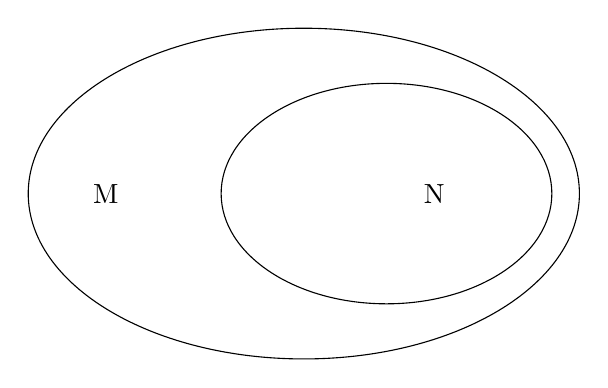
\begin{tikzpicture}[scale=0.7]
    \draw (0.0,0.0) ellipse (5.0 and 3.0);
    \draw (1.5,0.0) ellipse (3.0 and 2.0);
    \draw (-4.0,0.0) node[right]{M};
    \draw (2.0,0.0) node[right]{N};
  \end{tikzpicture}
  \caption{Teilmenge}
  \label{Abb:Mng:Teilmenge}
\end{center}
\end{figure}

Diese Abbildungen heißen 
\Begriff{Mengendiagramm}e oder auch \Begriff{Euler-Diagramm}e
\index[names]{Euler, Leonhard}\footnote{Leonhard Euler (1707-1783), 
schweizer Mathematiker,
\url{https://de.wikipedia.org/wiki/Leonhard_Euler}} oder 
\Begriff{Venn-Diagramm}e\index[names]{Venn, John}\footnote{John Venn
(1834-1923), englischer Logiker 
\url{https://de.wikipedia.org/wiki/John_Venn}}. Die 
Mengendiagramme dienen nur der Veranschaulichung! Sie können einem beim 
Beweisen als Anschauung helfen, sie ersetzen jedoch keinen Beweis!
\end{Unit}
\Translation{Mengendiagramm}{Venn diagram}

%% -----------------------------------------------------------------------------
\begin{Unit}[Bemerkung]
Aus der Definition der Gleichheit für Mengen und der Definition für Teilmengen 
ergibt sich

\begin{Bemerkung}
  Es seien $M$ und $N$ Mengen, dann gilt:
  \begin{align}
    (M = N) \Leftrightarrow (M \subseteq N) \wedge (N \subseteq M)\ .
  \end{align}
\end{Bemerkung}

Beweis: \newline
\begin{tabular}{l l l}
  & $M = N$ &\\
    $\Leftrightarrow$ & & (Definition der Gleichheit) \\
  & $\forall x : (x \in N) \leftrightarrow (x \in M)$ & \\
    $\Leftrightarrow$ & & (Aussagenlogik) \\
  & $\forall x : (x \in N) \rightarrow (x \in M)) \land$ & \\
  & $\forall x : (x \in M) \rightarrow (x \in N))$ & \\
    $\Leftrightarrow$ & & (Definition der Teilmenge) \\
  & $(N \subseteq M) \land (M \subseteq N)$ \ . & \\
\end{tabular}
 
\qed

Für den Beweis einer Mengengleichheit wird oftmals nachgewiesen, dass sich 
die beiden Mengen gegenseitig als Teilmengen enthalten.
\end{Unit}

%% -----------------------------------------------------------------------------
\begin{Unit}[Bemerkung]
Die Teilmengenbeziehung ist transitiv.
\begin{Bemerkung}
  Es seien $L$, $M$ und $N$ Mengen, dann gilt (Transitivität):
  \begin{align}
    (N \subseteq M) \wedge (M \subseteq L) \rightarrow\ (N \subseteq L)\ .
  \end{align}
  Ist $N$ eine Teilmenge von $M$ und $M$ eine Teilmenge von $L$, dann ist $N$ 
  auch eine Teilmenge von $L$.
\end{Bemerkung}

\begin{figure}[htbp]
\begin{center}
  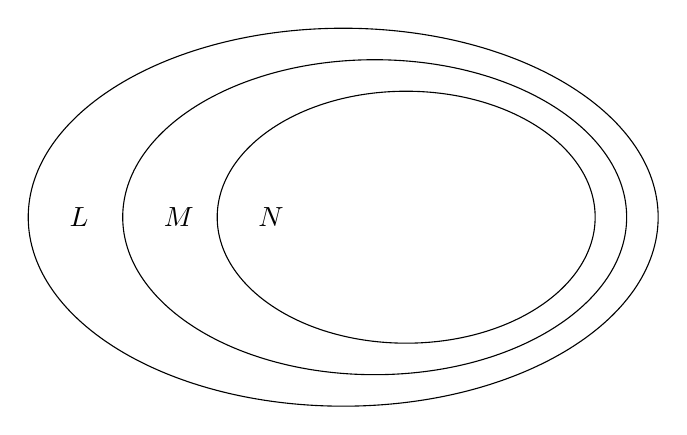
\begin{tikzpicture}[scale=0.8]
    \draw (0.0,0.0) ellipse (5.0 and 3.0);
    \draw (0.5,0.0) ellipse (4.0 and 2.5);
    \draw (1.0,0.0) ellipse (3.0 and 2.0);
    \draw (-4.5,0.0) node[right]{$L$};
    \draw (-3.0,0.0) node[right]{$M$};
    \draw (-1.5,0.0) node[right]{$N$};    
  \end{tikzpicture}
  \caption{Transitive Teilmengen}
  \label{Abb:Mng:Transitive Teilmengen}
\end{center}
\end{figure}

Beweis: Die Grafik (siehe Abbildung \ref{Abb:Mng:Transitive Teilmengen}) 
dient nur der Veranschaulichung. Der formale Beweis ist kurz. Für jedes 
$x \in N$ gilt:

\begin{tabular}{l l | l}
  & $(x \in N)$ &  \\
  $\Rightarrow$ & & $N$ ist Teilmenge von $M$ ($N \subseteq M$) \\
  & $(x \in M)$ & \\
  $\Rightarrow$ & & $M$ ist Teilmenge von $L$ ($M \subseteq L$) \\
  & $(x \in L)$ & \\
\end{tabular} 

\qed
\end{Unit}

%% -----------------------------------------------------------------------------
\begin{Unit}[Uebung]
Es seien $M\ =\ \{1, 2\}$ und $N\ =\ \{2, 3, 4\}$. Welche der folgenden 
Aussagen sind richtig?
\begin{itemize}
  \item $M \subseteq N$? \\
    Nein, da $1 \in M$, aber $1 \notin N$.
  \item $N \subseteq M$? \\
    Nein, da $4 \in N$, aber $4 \notin M$.
  \item $M\ =\ N$? \\
    Nein, da $4 \in N$, aber $4 \notin M$.
  \item $M\ \not=\ N$? \\
    Ja.
  \item $\{2, 4\}\ \subseteq N$? \\
    Ja.
  \item $2\ \in\ M$? \\
    Ja.
  \item $2\ \subseteq\ M$? \\
    Nein, dies ist nicht einmal ein gültiger Ausdruck, da $2$ keine Menge 
    ist, so dass keine Teilmengenbeziehung bestehen kann. Gültig wären die 
    Aussagen  $2\ \in\ M$ oder $\{2\} \subseteq\ M$.
  \item $\{2, \{3, 4\}\}\ \subseteq N$? \\
    Nein, die Menge auf der linken Seite besteht aus zwei Elementen, aus der 
    $2$ und aus der Menge mit den Elementen $3$ und $4$. Das zweite Element 
    ($\{3,4\}$) ist jedoch kein Element von $N$ (sondern eine Teilmenge von 
    $N$). Für die Teilmengenbeziehung müsste es jedoch Element von $N$ sein.
\end{itemize}
\end{Unit}

%% --- Potenzmenge -------------------------------------------------------------
%\subsection*{Potenzmenge}

%% -----------------------------------------------------------------------------
\begin{Unit}[Definition Potenzmenge]
Die Teilmengen einer Menge lassen sich selber wiederum zu einer Menge
zusammenfassen.

\begin{Definition}
Die Mengen aller Teilmengen einer Menge $M$ heißt \Begriff{Potenzmenge} von 
$M$: $\mathcal{P}(M)$.
\begin{align}
  \mathcal{P}(M) := \{T \mid T \subseteq M\}
\end{align}
\end{Definition}
\end{Unit}
\Translation{Potenzmenge}{power set}

%% -----------------------------------------------------------------------------
\begin{Unit}[Beispiel] \ 
\begin{enumerate}
  \item Es sei $M = \varnothing$, also die leere Menge, dann ist 
    $\mathcal{P}(M) = \{\varnothing\}$, also die Menge, die nur ein Element 
    hat, nämlich die leere Menge. Zu beachten ist, dass $\mathcal{P}(M)$ nicht 
    die leere Menge ist, sondern die Menge, die nur aus der leeren Menge 
    besteht!

  \item Es sei $M = \{a\}$ eine Menge, die aus einem Element besteht. Damit 
    ist die Potenzmenge die Menge, die aus der leeren Menge und der Menge 
    selbst besteht, denn das sind die einzigen Teilmengen der Menge $M$, also 
    $\mathcal{P}(M) = \{ \varnothing, M \}$.

  \item Es sei $M = \{a, b\}$ eine Menge mit genau zwei Elementen, dann ist 
    $\mathcal{P}(M) = \{ \varnothing, \{a\}, \{b\}, M \}$.
\end{enumerate}
\end{Unit}

%% -----------------------------------------------------------------------------
\begin{Unit}[Bemerkung]
Für endliche Mengen kann die Elementanzahl der Potenzmenge einfach angegeben
werden.

\begin{Bemerkung}
  Es sei $M$ eine endliche Menge mit $n = |M|$ Elementen, dann hat die 
  Potenzmenge von $M$ genau $2^n$ Elemente.
  \begin{align}
    ( |M| = n ) \rightarrow ( |\mathcal{P}(M)| = 2^n )
  \end{align}
\end{Bemerkung}

Der Beweis kann durch vollständige Induktion geführt werden, was hier jedoch 
nicht ausgeführt wird.
\end{Unit}

%% -----------------------------------------------------------------------------
\begin{Unit}[Bemerkung]
Eine Teilmengenbeziehung überträgt sich auch auf die Potenzmengen.

\begin{Bemerkung}
  Es seien $M$ und $N$ zwei beliebige Mengen. Ist $M$ eine Teilmenge von $N$, 
  dann ist die Potenzmenge von $M$ eine Teilmenge der Potenzmenge von $N$.
  \begin{align}
    M \subseteq N\ \rightarrow\ \mathcal{P}(M) \subseteq \mathcal{P}(N) 
  \end{align}
\end{Bemerkung}
Beweis: als Übung
\end{Unit}

%%------------------------------------------------------------------------------
%% Abschnitt: Operationen von Mengen
%%------------------------------------------------------------------------------
\section{Operationen von Mengen}
\label{sec:Mengen:Operationen von Mengen}

Wie kann mit Mengen gerechnet werden, welche Operationen gibt es und welche 
Regeln gibt es für die Operationen gibt.

%% --- Durchschnitt und Vereinigung --------------------------------------------
%\subsection*{Durchschnitt und Vereinigung}

%% -----------------------------------------------------------------------------
\begin{Unit}[Definition Durchschnitt]
Eine wichtige Verknüpfung von Mengen ist der Durchschnitt.

\begin{Definition}
  Es seien $M$ und $N$ beliebige Mengen. 
  Die Menge der Elemente, die sowohl in der Menge $M$, als auch in der Menge 
  $N$ sind, heißt der \Begriff{Durchschnitt} ($M \cap N$) von $M$ und $N$.
  \begin{align}
    M \cap N\ := \{ x \mid (x\in M) \land (x \in N) \}
  \end{align}
\end{Definition}
\Translation{Durchschnitt}{intersection}

\begin{figure}[htbp]
\begin{center}
  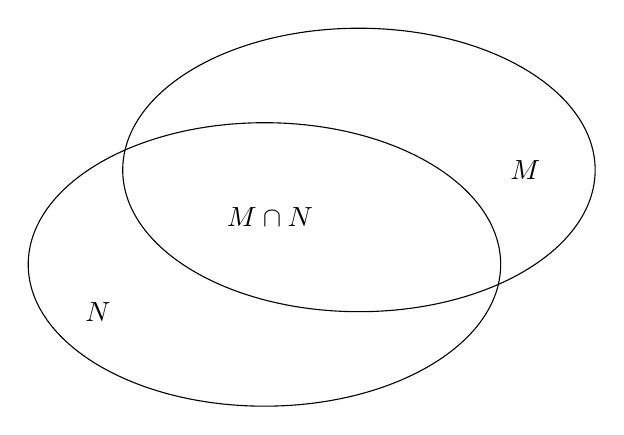
\begin{tikzpicture}[scale=0.6]
    \draw (0.0,0.0) ellipse (5.0 and 3.0);
    \draw (2.0,2.0) ellipse (5.0 and 3.0);
    \draw (-4.0,-1.0) node[right]{$N$};
    \draw (5.0,2.0) node[right]{$M$};
    \draw (-1.0,1.0) node[right]{$M \cap N$};
  \end{tikzpicture}
  \caption{Durchschnitt von Mengen}
  \label{Abb:Mng:Durchschnitt von Mengen}
\end{center}
\end{figure}

Die Abbildung (siehe \ref{Abb:Mng:Durchschnitt von Mengen}) veranschaulicht 
den Durchschnitt. Der Durchschnitt der Mengen $M$ und $N$ beinhaltet nur die 
kleine innere Fläche, die mit $M \cap N$ bezeichnet ist. 
\end{Unit}

%% -----------------------------------------------------------------------------
\begin{Unit}[Definition Vereinigung]
Eine weitere wichtige Verknüpfung von Mengen ist die Vereinigung.

\begin{Definition}
  Es seien $M$ und $N$ beliebige Mengen. 
  Die Menge der Elemente, die in der Menge $M$ oder in der Menge $N$ sind, 
  heißt die \Begriff{Vereinigung} ($M \cup N$) von $M$ und $N$.
  \begin{align}
    M \cup N := \{ x \mid (x \in M) \lor (x \in N) \}
  \end{align}
\end{Definition}
\Translation{Vereinigung}{union}
\end{Unit}

%% -----------------------------------------------------------------------------
\begin{Unit}[Definition disjunkt]
Die Eigenschaft, dass der Durchschnitt zweier Mengen die leere Menge ist, ist
eine besondere Eigenschaft.
 
\begin{Definition}
  Sind $M$ und $N$ zwei beliebige Mengen, mit leerem Durchschnitt ($M \cap N
  = \varnothing$), dann heißen $M$ und $N$ \Begriff{disjunkt}, und es wird 
  statt $M \cup N$ auch $M + N$ geschrieben.
\end{Definition}
\Translation{disjunkt}{disjoint}
\end{Unit}

%% --- Verallgemeinerter Durchschnitt und Vereinigung --------------------------
%\subsection*{Verallgemeinerter Durchschnitt und Vereinigung}

%% -----------------------------------------------------------------------------
\begin{Unit}[Anmerkung]
Durchschnitt und Vereinigung lassen sich nicht nur für zwei Mengen definieren. 
Ist $I$ eine beliebige (endliche oder unendliche) Indexmenge und ist jedem $i 
\in I$ eine Menge $M_i$ zugeordnet, so wird der \Begriff
{verallgemeinerten Durchschnitt} der Mengen $M_i$ mittels
\begin{align}
  \bigcap_{i \in I} M_i := \{ x \mid \forall i \in I: x \in M_i \} .
\end{align}
definiert.
Es ist die Menge der Elemente, die in jeder der Mengen $M_i$ enthalten ist.

Weiter wird definiert
\begin{align}
  \bigcup_{i \in I} M_i := \{x \mid \exists i \in I: x \in M_i \}
\end{align} die \Begriff{verallgemeinerte Vereinigung} der Mengen $M_i$. 
Es ist die Menge der Elemente, die in mindestens einer der Mengen $M_i$ 
enthalten ist.

Ist die Indexmenge gleich der leeren Menge, so ist der Durchschnitt die 
Grundmenge (!) und die Vereinigung die leere Menge (!), da die Bedingung 
$i \in I$ nicht erfüllt ist.
\end{Unit}

%% --- Assoziativ-, Kommutativ- und Distributivgesetz --------------------------
%\subsection*{Assoziativ-, Kommutativ- und Distributionsgesetz}

%% -----------------------------------------------------------------------------
\begin{Unit}[Satz]
Für das Rechnen mit Mengen gelten folgende Aussagen:

\begin{Satz}[Assoziativ-, Kommutativ- und Distributionsgesetz]
  Gegeben seien die Mengen $M$, $N$ und $L$ beliebige Mengen.
  Dann gelten die \Begriff{Assoziativgesetz}e
  \begin{align}
    M \cup (N \cup L) = (M \cup N) \cup L \\ 
    M \cap (N \cap L) = (M \cap N) \cap L\ ,
  \end{align}
  die \Begriff{Kommutativgesetz}e 
  \begin{align}
    M \cup N = N \cup M \\
    M \cap N = N \cap M
  \end{align}
  und die \Begriff{Distributivgesetz}e
  \begin{align}
    M \cup (N \cap L) = (M \cup N) \cap (M \cup L) \\
    M \cap (N \cup L) = (M \cap N) \cup (M \cap L) \ .
  \end{align}
\end{Satz}
\Translation{Assoziativgesetz}{associative law}
\Translation{Kommutativgesetz}{commutative law}
\Translation{Distributivgesetz}{distributive law}

Mit Hilfe der Mengendiagramme (siehe Abbildung \ref{Abb:Mng:Mengendiagramm}) 
lassen sich diese Sätze leicht veranschaulichen.

\begin{figure}[htbp]
\begin{center}
  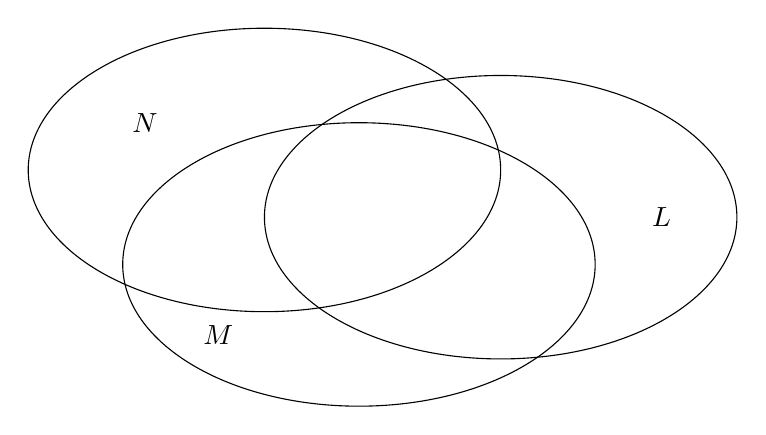
\begin{tikzpicture}[scale=0.6]
    \draw (0.0,0.0) ellipse (5.0 and 3.0);
    \draw (-2.0,2.0) ellipse (5.0 and 3.0);
    \draw (3.0,1.0) ellipse (5.0 and 3.0);
    \draw (-3.5,-1.5) node[right]{$M$};    
    \draw (-5.0,3.0) node[right]{$N$};
    \draw (6.0,1.0) node[right]{$L$};
  \end{tikzpicture}
  \caption{Mengendiagramm}
  \label{Abb:Mng:Mengendiagramm}
\end{center}
\end{figure}

Formal wird das Distributivgesetz bewiesen.

\begin{tabular}{l l | l}
    & $x \in M \cap (N \cup L)$ & \\
$\leftrightarrow$ & & (Definition Durchschnitt) \\
    & $(x\in M) \land (x \in (N \cup L))$ &  \\
$\leftrightarrow$ & & (Definition Vereinigung) \\
    & $(x\in M) \land ((x \in N) \lor (x\in L))$ & \\
$\leftrightarrow$ & & (Distributivgesetz - Aussagen) \\
    & $((x\in M) \land (x \in N)) \lor $ & \\
                  & $((x \in M) \land (x \in L))$ & \\
$\leftrightarrow$ & & (Definition Durchschnitt) \\
    & $(x \in M \cap N) \lor (x \in M \cap L)$ & \\
$\leftrightarrow$ & & (Definition Vereinigung) \\
    & $x \in (M \cap N) \cup (M \cap L)$ & \\
\end{tabular}

Somit wurde gezeigt, dass jedes Element $x \in M \cap (N \cup L)$ auch Element
von $(M \cap N) \cup (M \cap L)$, also $M \cap (N \cup L) \subseteq (M \cap N) 
\cup (M \cap L)$ und umgekehrt. Damit ist die beidseitige 
Teilmengenbeziehung gezeigt, und somit die Identität der beiden Mengen.\qed

Das Assoziativgesetz gilt nicht nur für drei Mengen, sondern auch für mehre 
Mengen. Daher kann hierbei auf die Klammersetzung verzichtet werden.
\end{Unit}

%% -----------------------------------------------------------------------------
\begin{Unit}[Bemerkung]
Für das Rechnen mit Mengen sind folgende Regeln oftmals nützlich:
\begin{Bemerkung}
  Es seien $M$ und $N$ beliebige Mengen, dann gelten
  \begin{align}
    M \cap (M \cup N) &= M \\
    M \cup (M \cap N) &= M \\
    M \cap M &= M \\
    M \cup M &= M
  \end{align}
\end{Bemerkung}
\end{Unit}

%% -----------------------------------------------------------------------------
\begin{Unit}[Bemerkung]
Für die leere Menge und die Grundmenge gelten folgende Aussagen:
\begin{Bemerkung}
  Es sei $M$ eine beliebige Teilmenge der Grundmenge $G$, dann gelten
  \begin{align}
    M \cap \varnothing &= \varnothing \\
    M \cup \varnothing &= M \\
    M \cap G &= M \\
    M \cup G &= G
  \end{align}
\end{Bemerkung}
\end{Unit}

%% --- Durchschnitt und Vereinigung bei Potenzmengen  --------------------------
%\subsection*{Durchschnitt und Vereinigung bei Potenzmengen}

%% -----------------------------------------------------------------------------
\begin{Unit}[Bemerkung]
Wie wirken sich der Durchschnitt und die Vereinigung von zwei Mengen auf die 
Potenzmengen aus, welchen Beziehungen gibt es?

\begin{Bemerkung}
  Es seien $M$ und $N$ zwei beliebige Mengen. Dann gelten \\
  (a) Die Potenzmenge des Durchschnitts der Mengen $M$ und $N$ ist gleich 
  dem Durchschnitt der Potenzmengen der Mengen $M$ und $N$.
  \begin{align}
    \mathcal{P}(M \cap N) = \mathcal{P}(M) \cap \mathcal{P}(N) 
  \end{align}
  (b) Die Vereinigung der Potenzmengen der Mengen $M$ und $N$ ist eine 
  Teilmenge der Potenzmenge der Vereinigung der Mengen $M$ und $N$.
  \begin{align}
    \mathcal{P}(M) \cup \mathcal{P}(N) \subseteq \mathcal{P}(M \cup N) 
  \end{align}
\end{Bemerkung}

Beweis: Übung. Bei (a) ist die gegenseitige Teilmengenbeziehung zu zeigen. 
Bei (b) ist nur die eine Richtung nachzuweisen. Wieso gilt die Gegenrichtung 
nicht? Finden Sie dazu ein Gegenbeispiel.
\end{Unit}

%% --- Durchschnitt und Vereinigung bei Potenzmengen  --------------------------
%\subsection*{Differenz und Komplement}

%% -----------------------------------------------------------------------------
\begin{Unit}[Definition Differenz, Komplement]
Im nachfolgenden seien $M$, $N$ und $L$ stets beliebige Mengen, die Teilmenge
einer festen Grundmenge $G$ sind.

\begin{Definition}
  (a) Es seien $M$ und $N$ beliebige Mengen, dann heißt
    \begin{align}
      M \backslash N := \{ x \mid (x \in M) \land (x \notin N) \} 
    \end{align}
    die \Begriff{Differenz} der Mengen $M$ und $N$. In der Differenz sind
    die Elemente von $M$, die nicht in $N$ sind. \\
  (b) Es sei $M$ eine beliebige Teilmenge von $G$, dann heißt die Menge
    \begin{align}
      \complement_G(M) := \{ x \in G \mid x \notin M \} = G \backslash  M
    \end{align}
    das \Begriff{Komplement} von $M$ bezüglich $G$. Es enthält die Elemente 
    der Grundmenge, die nicht in $M$ sind.
\end{Definition}
\Translation{Differenz}{difference}
\Translation{Komplement}{complementon}

Ist die Grundmenge $G$ allgemein bekannt, so kann das Komplement einer Menge 
$M$ kurz als $\overline{M}$ geschrieben werden. Durch die Umformulierung 
$\complement_G(M) := \{ x \in G \mid \neg(x \in M) \}$ wird der Zusammenhang 
zwischen Komplementbildung und der aussagenlogischen Negation deutlich.

Es ergibt sich sofort, dass $M$ und $\complement_G(M)$ disjunkt sind und dass 
$M + \complement_G(M) = G$ ist.
\end{Unit}

%% -----------------------------------------------------------------------------
\begin{Unit}[Bemerkung]
Wie wird die Differenzmenge mit Hilfe der Komplementmenge gebildet.

\begin{Bemerkung} 
  Es seien $M$ und $N$ beliebige Teilmengen einer Grundmenge $G$, dann gilt
  \begin{align}
    M \backslash N = M \cap \complement_G(N) \ .
  \end{align}
\end{Bemerkung}
Beweis: Übung
\end{Unit}

%% -----------------------------------------------------------------------------
\begin{Unit}[Definition symmetrische Differenz]
Wie wird die symmetrische Differenz mit Hilfe der Differenzen gebildet.

\begin{Definition}
  Es seien $M$ und $N$ Mengen, dann heißt
  \begin{align}
    M  \triangle N\ := (M \backslash N) + (N \backslash M) 
  \end{align}
  die \Begriff{symmetrische Differenz}\index{Differenz, symmetrische} 
  von $M$ und $N$.
\end{Definition}
\Translation{symmetrische Differenz}{symmetric difference}
Veranschaulichen Sie sich die Differenz.
\end{Unit}

%% -----------------------------------------------------------------------------
\begin{Unit}[Bemerkung]
Nochmals eine andere Möglichkeit, die symmetrische Differenz darzustellen.

\begin{Bemerkung} 
  Es seien $M$ und $N$ beliebige Teilmengen, dann gilt 
  \begin{align}
    M \triangle N = (M \cup N) \backslash (M \cap N) \ .
  \end{align}
\end{Bemerkung}
Beweis: Übung
\end{Unit}

%% --- Regeln von de Morgan ----------------------------------------------------
%\subsection*{Regeln von de Morgan}

%% -----------------------------------------------------------------------------
\begin{Unit}[Regel von de Morgan]
Wie bei den Aussagen gibt es auch hier Regeln von de Morgan.

\begin{Satz}
  Es seien $M$ und $N$ beliebige Teilmengen der Grundmenge $G$, dann gelten 
  die Sätze von de Morgan\index[names]{Morgan, Augustus de}\footnote{Augustus 
  de Morgan (1806-1871), englischer Mathematiker
(\url{https://de.wikipedia.org/wiki/Augustus_De_Morgan})} 
  \begin{align}
    \complement_G(M \cup N) &= \complement_G(M) \cap \complement_G(N) \\
    \complement_G(M \cap N) &= \complement_G(M) \cup \complement_G(N) \ .
  \end{align}
\end{Satz}

Ist die Grundmenge G bekannt, so wird kurz
\begin{align}
  \overline{(M \cup N)} &= \overline{M} \cap \overline{N} \text{ und } \\
  \overline{(M \cap N)} &= \overline{M} \cup \overline{N} 
\end{align}
geschrieben.

Beweis der ersten Aussage:\\
\begin{tabular}{l l | l}
                  & $x \in \complement_G(M \cup N)$ & \\
$\leftrightarrow$ & & (Definition Komplement) \\
                  & $(x \in G) \land (x \notin (M \cup N))$ & \\
$\leftrightarrow$ & & (Negation) \\
                  & $(x \in G) \land\neg (x \in (M \cup N))$ & \\
$\leftrightarrow$ & & (Definition Vereinigung) \\
                  & $(x \in G) \land$ & \\
                  &  $\neg((x \in M) \lor (x \in N))$ & \\
$\leftrightarrow$ & & (Satz von de Morgan - Aussagen) \\
                  & $(x \in G) \land $ &  \\
                  & $((\neg(x \in M)) \land (\neg(x \in N)))$ &  \\
$\leftrightarrow$ & & (Assoziativgesetz) \\
                  & $((x \in G) \land (\neg(x \in M)))$ & \\
                  & $\land ((x \in G) \land (\neg(x \in N)))$ & \\
$\leftrightarrow$ & & (Negation) \\
                  & $((x \in G) \land (x \notin M)) $ & \\
                  & $\land ((x \in G) \land (x \notin N)) $ & \\
$\leftrightarrow$ & & (Definition Komplement) \\
                  & $(x \in \complement_G(M) \land (x \in \complement_G(N))$ 
                    & \\
$\leftrightarrow$ & & (Definition Durchschnitt) \\
                  & $x \in \complement_G(M) \cap \complement_G(N)$ & \\
\end{tabular}

Auf Grund der Definition der Mengengleichheit gilt damit die behauptete 
Aussage. Der andere Teil kann analog bewiesen werden.
\qed
\end{Unit}

%% -----------------------------------------------------------------------------
\begin{Unit}[Anmerkung]
Auch für Familien von Mengen gelten die verallgemeinerter Sätze von de Morgan
\index[names]{Morgan, Augustus de}.
\begin{align}
  \complement_G(\bigcap_{i \in I}M_i) = \bigcup_{i \in I}\complement_G(M_i) \\
  \complement_G(\bigcup_{i \in I}M_i) = \bigcap_{i \in I}\complement_G(M_i)
\end{align}
\end{Unit}
%%------------------------------------------------------------------------------

%%------------------------------------------------------------------------------
%% Abschnitt: Klasseneinteilung
%%------------------------------------------------------------------------------
\section{Klasseneinteilung}
\label{sec:Mengen:Klasseneinteilung}

%% -----------------------------------------------------------------------------
\begin{Unit}[Definition Klasseneinteilung]
Im folgenden sei $I$ stets eine beliebige Indexmenge.

\begin{Definition}
  Es sei $\{M_i \mid i \in I)\}$ eine Familie von beliebigen nicht leeren 
  Teilmengen einer Grundmenge. Die Familie von Mengen heißt 
  \textbf{(paarweise) disjunkt}\index{disjunkt, paarweise}, wenn für alle 
  $i, j \in I$ die Mengen $M_i$ und $M_j$ disjunkt sind: 
  \begin{align}
    \{ M_i \mid i \in I \} \text{ paarweise disjunkt} :\Leftrightarrow\
      \forall i,j \in I, i \not= j: M_i \cap M_j = \varnothing \ .
  \end{align} 
  Eine Familie von Mengen heißt \Begriff{Klasseneinteilung} oder 
  \Begriff{disjunkte Zerlegung}\index{Zerlegung, disjunkte} oder 
  \Begriff{Partition} von $G$, wenn sie paarweise disjunkt ist und die 
  verallgemeinerte Vereinigung der Mengen gleich der Grundmenge ist.
\end{Definition}
\Translation{paarweise disjunkt}{pairwise disjoint}
\Translation{Klasseneinteilung}{partition}
\Translation{Zerlegung}{partition}

\begin{figure}[htbp]
\begin{center}
  \begin{tikzpicture}
    \draw (0,0) -- (0,4) -- (8,4) -- (8,0) -- (0,0);
    \draw (2,0) -- (2,4);
    \draw (4,0) -- (4,4);
    \draw (6,0) -- (6,4);
    \draw (2,2) -- (6,2);
    \draw (0,2) node[right]{$M_1$};    
    \draw (2,3) node[right]{$M_2$};
    \draw (2,1) node[right]{$M_3$};
    \draw (4,3) node[right]{$M_4$};
    \draw (4,1) node[right]{$M_5$};
    \draw (6,2) node[right]{$M_6$};
  \end{tikzpicture}
  \caption{Klasseneinteilung}
  \label{Abb:Mng:Klasseneinteilungn}
\end{center}
\end{figure}

Klasseneinteilungen treten an vielen Stellen auf. In Abbildung 
\ref{Abb:Mng:Klasseneinteilungn} ist eine Klasseneinteilung dargestellt:
paarweise disjunkt, die Vereinigung ist die komplette Grundmenge.
\end{Unit}

%% -----------------------------------------------------------------------------
\begin{Unit}[Beispiel]
  Die natürlichen Zahlen lassen sich in die disjunkten Mengen der geraden und 
  der ungeraden Zahlen zerlegen.
\end{Unit}

%% -----------------------------------------------------------------------------
\begin{Unit}[Beispiel]
  Ist $P$ die Menge der Produktion der Automobile eines Werkes an einem Tag. 
  Es werden die verschiedenen Baumuster $B_1,\ldots, B_n$ produziert und 
  seien $T_1, \ldots, T_n$ die Menge der Autos der Tagesproduktion mit diesen 
  Baumustern, dann ist $\{T_i\ ;\ i = 1,\ldots,n\}$ die Klasseneinteilung der 
  Tagesproduktion $P$.
\end{Unit}

%% -----------------------------------------------------------------------------
\begin{Unit}[Definition Äquivalenzklassen]
Durch die Klasseneinteilung einer Menge $G$ ist jedes Element von $G$ genau 
in einer Teilmenge der Klasseneinteilung enthalten.

\begin{Definition}
  Sind zwei Elemente $x$, $y$ in der gleichen Teilmenge einer 
  Klasseneinteilung, so heißen sie \Begriff{äquivalent} ($x \sim y$). Die 
  Teilmengen der Klasseneinteilung heißen auch \Begriff{Äquivalenzklassen}. 
  Ein Element einer Äquivalenzklasse heißt \Begriff{Repräsentant} der
  Äquivalenzklasse.
\end{Definition}
\end{Unit}
\Translation{äquivalent}{equivalent}
\Translation{Äquivalenzklasse}{equivalence class}
\Translation{Repräsentant}{representative}

%% -----------------------------------------------------------------------------
\begin{Unit}[Bemerkung]
Für Äquivalenzklassen gibt es einige Eigenschaften, die bei der Behandlung 
von Relationen noch genauer betrachtet werden.
 
\begin{Bemerkung}
  Es seien $x$, $y$ und $z$ Elemente aus einer Menge $G$ mit einer 
  Klasseneinteilung. Für die Äquivalenz $\sim$ der Klasseneinteilung 
  gelten: \\
  (a) Für jedes $x \in G$ ist $x \sim x$, das heißt, dass die 
    Klasseneinteilung \Begriff{reflexiv} ist. \\
  (b) Ist $x \sim y$, sind also $x$ und $y$ in derselben Äquivalenzklasse, 
    dann gilt auch $y \sim x$, das heißt, dass die Klasseneinteilung 
    \Begriff{symmetrisch} ist. \\
  (c) Ist $x \sim y$ und $y \sim z$, dann ist auch $x \sim z$, das heißt, 
    dass die Klasseneinteilung \Begriff{transitiv} ist.
\end{Bemerkung}
\end{Unit}
\Translation{reflexiv}{reflexive}
\Translation{symmetrisch}{symmetric}
\Translation{transitiv}{transitive}

%% -----------------------------------------------------------------------------
\begin{Unit}[Beispiel]
  Die Menge der ganzen Zahlen $\ZZ$ wird bezüglich des Rests bei der Division 
  durch $6$ in sechs verschiedene Äquivalenzklassen aufgeteilt. Für 
  $i = 0, 1, 2, 3, 4, 5$ seien $T_i$ die Menge der ganzen Zahlen, die bei der
  Division durch $6$ den Rest $i$ haben. 
  \begin{align}
    T_i = \{x \in \ZZ \mid \exists n \in \ZZ : x = 6n + i \}
  \end{align}
  Dies definiert eine Klasseneinteilung: $\ZZ = T_0 + T_1 + T_2 + T_3 + T_4 + 
    T_5$. \\
  Für einen Repräsentanten und jeden Vertreter einer der Klassen $T_2$, $T_4$ 
  oder $T_6$ gilt, dass er durch zwei teilbar ist. Die Repräsentanten der 
  Klassen $T_3$ und $T_6$ sind jeweils durch 3 teilbar. Daher können in den 
  Klassen $T_2$, $T_3$, $T_4$ und $T_6$ keine Primzahlen enthalten sein 
  (Ausnahme: $2$ und $3$ selbst). Durch die gemeinsame Eigenschaft der Zahlen 
  der Klassen kann dies für jedes Element der Klasse bewiesen werden.
\end{Unit}

%% -----------------------------------------------------------------------------
\begin{Unit}[Anmerkung]
Ist $n$ eine beliebige natürliche Zahl, so kann die Menge $\ZZ$ in $n$ 
disjunkte Teilmengen bezüglich der Division durch $n$ zerlegt werden. Die 
Teilmengen $T_i$ für $i = 0, 1, \ldots, n-1$, werden folgendermaßen gebildet: 
\begin{align}
  T_i := \{ x \in \ZZ \mid \exists k \in \ZZ: x = kn+i \}
\end{align}
Diese Teilmengen bilden eine Klasseneinteilung der ganzen Zahlen. Die Menge 
$\ZZ_n = \{0, 1, \ldots, n-1\}$ bildet ein Repräsentantensystem. Dieses 
Repräsentantensystem wird im Folgenden noch vorkommen. Es hat eine wichtige
Bedeutung in der Informatik.
\end{Unit}

%% -----------------------------------------------------------------------------
\begin{Unit}[Anmerkung]
Die Klassenaufteilung ist ein häufig verwendetes Verfahren, um die 
Problemlösung oder andere Aufgaben auf eine begrenzte Zahl von Fällen zu 
reduzieren. Bei Meinungsumfragen werden die Befragten in bestimmte Klassen
eingeteilt, um dann Aussagen über die Vertreter dieser Klassen im allgemeinen 
zu erhalten.

Auch die Fallunterscheidungen ist eine Klasseneinteilung. Auch 
Fallunterscheidungen kommen an vielen Stellen vor, zum Beispiel bei der 
Definition von mathematischen Funktionen, bei der Berechnung der privaten 
Steuerlast, in Programmvorgaben, um nur einige wenige Beispiele  zu nennen.
\end{Unit}

%%------------------------------------------------------------------------------

%%------------------------------------------------------------------------------
%% Abschnitt: Kartesisches Produkt
%%------------------------------------------------------------------------------
\section{Kartesisches Produkt}
\label{sec:Mengen:Kartesisches Produkt}

%% -----------------------------------------------------------------------------
\begin{Unit}[Anmerkung]
In vielen Fällen ist es sinnvoll, geordnete Paare $(x, y)$ von Elementen $x \in 
X$ und $y \in Y$ zweier Mengen $X$ und $Y$ zu betrachten. Dabei heißt $x$ die
erste Komponente und $y$ die zweite Komponente. Ein Beispiel hierfür ist das 
2-dimensionale Koordinatensytem, bei dem $X = \RR$ und $Y = \RR$ gilt. Die 
Gleichheit zweier geordneter Paare wird durch
\begin{align}
  (x_1,y_1) = (x_2,y_2) :\Leftrightarrow (x_1 = x_2) \land (y_1 = y_2)
\end{align}
definiert. Die Mengen $X$ und $Y$ können jedoch auch beliebige Mengen sein.
\end{Unit}

%% -----------------------------------------------------------------------------
\begin{Unit}[Definition Kartesisches Produkt für zwei Mengen]
Zuerst die Definition eines kartesischen Produktes bei zwei Mengen. 

\begin{Definition}
  Es seien $X$ und $Y$ zwei beliebige Mengen, dann heißt die Menge
  \begin{align}
    X \times Y := \{ (x,y) \mid x \in X \land y \in Y \} \ ,
  \end{align}
  also die Menge der geordneten Paare $(x,y)$ mit $x \in X$ und $y \in Y$ das
  \Begriff{kartesische Produkt} der Mengen $X$ und $Y$. Die Elemente 
  dieses kartesischen Produktes heißen auch \Begriff{geordnete 2-Tupel}
  \index{Tupel, geordnetes 2-}.
\end{Definition}
\Translation{kartesisches Produkt}{Cartesian product}
\Translation{Tupel}{tuple}

Das kartesische Produkt ist nach Ren\`{e} Descartes\footnote{Ren\`{e} 
Descartes (1596-1650) französischer Philosoph und Mathematiker,
\url{https://de.wikipedia.org/wiki/Ren\%C3\%A9_Descartes}} 
\index[names]{Descartes, Ren\`{e}} benannt. Das kartesische Produkt ist 
selber wieder eine Menge, deren Elemente die geordneten 2-Tupel sind.
\end{Unit}

%% -----------------------------------------------------------------------------
\begin{Unit}[Beispiel]
In der Regel ist $X \times Y$ ungleich $Y \times X$. Die Gleichheit ist
hier die Mengengleichheit. Diese Aussage kann anhand des ersten Beispiel
sofort gesehen werden.

  Es seien $X = \{1, 2, 3\}$ und $Y = \{a, b\}$, dann ist
  \begin{align}
    X \times Y = \{ (1,a), (1,b), (2,a), (2,b), (3,a), (3,b) \}
  \end{align}
  und
  \begin{align}
    Y \times X = \{ (a,1), (a,2), (a,3), (b,1), (b,2), (b,3) \} \ .
  \end{align}
  Die beiden kartesischen Produkte sind ungleich.
\end{Unit}

%% -----------------------------------------------------------------------------
\begin{Unit}[Beispiel]
  Es seien $P = \{ p_1, p_2, p_3, p_4 \}$ eine Menge von Produkten und $L = 
  \{ l_1, l_2, l_3 \}$ eine Menge von Lieferanten. Dann ist $P \times L$ das 
  kartesische Produkt der Produkte und Lieferanten.
\end{Unit}

%% -----------------------------------------------------------------------------
\begin{Unit}[Beispiel]
  Es seien $X = Y = \NN$, dann ist $\NN \times \NN$ die Menge der geordneten 
  Paare von natürlichen Zahlen.
\end{Unit}

%% -----------------------------------------------------------------------------
\begin{Unit}[Beispiel]
  Es seien $X = Y = \RR$, dann ist $\RR \times \RR$ die Menge der geordneten 
  Paare von reellen Zahlen, der zweidimensionale Anschauungsraum.
\end{Unit}

%% -----------------------------------------------------------------------------
\begin{Unit}[Definition Kartesisches Produkt]
Die Definition des kartesischen Produktes kann verallgemeinert werden. Das 
Produkt kann auch für drei oder mehr Mengen gebildet werden.

\begin{Definition}
  Es sei $n \in \NN$ und $X_i$ ($i = 1, \ldots, n$) beliebige nicht leere 
  Mengen. Dann heißt die Menge
  \begin{align}
    \prod_{i=1}^n X_i := \{ (x_1, x_2, \ldots, x_n) \mid \forall_{i=1}^n x_i 
      \in X_i \} \ ,
  \end{align}
  die Menge aller (geordneten) $n$-Tupel $(x_1, x_2, \ldots, x_n)$ mit $x_i 
  \in X_i$ für alle $i \in \{1, 2, \ldots, n\}$, das \Begriff{kartesische 
  Produkt} von $X_1, X_2, \ldots , X_n$.
\end{Definition}

Statt $\prod_{i=1}^n X_i$ wird auch $X_1 \times X_2 \times \cdots \times 
X_n$ geschrieben. Die Definition kann auch auf Folgen von Mengen 
$\{ X_n \}_{n \in \NN}$ verallgemeinert werden.

Ist $n = 2$, so heißt $X_1 \times X_2$ auch \Begriff{Paarmenge}. Für 
$n = 1$ ist das kartesische Produkt gleich der Menge $X_1$. Sind $X_1 = X_2 = 
\cdots = X_n = X$, so wird für $\prod_{i=1}^n X_i$ auch kurz $X^n$ geschrieben. 
Beispiele für spezielle kartesische Produkte sind $\RR^2$ und $\RR^3$, die zwei- 
und dreidimensionalen Anschuungsräume.
\end{Unit}

%% -----------------------------------------------------------------------------
\begin{Unit}[Bemerkung]
Bei einem (endlichen) kartesisches Produkt von endlichen Mengen, kann die
Elementanzahl des kartesischen Produktes berechnet werden.

\begin{Bemerkung}
  Es seien für $n \in \mg{N}$ die Mengen $X_1, X_2, \ldots , X_n$ endlich mit 
  den Elementanzahlen $|X_i| = m_i$. Dann gilt $|\prod_{i=1}^n X_i| = 
  \prod_{i=1}^n m_i $.
\end{Bemerkung}
\end{Unit}

%%% =============================================================================
%% Mathematische Grundlagen - Grundbegriffe
%% Kapitel 05 - Relationen
%% Autor: Andreas Zeh-Marschke
%% Datum: 2025-03-30
%% =============================================================================

\chapter{Relationen}
\label{cha:Gdl-K05-Relationen}

%% -----------------------------------------------------------------------------
%\begin{unit}
Zu einem der fundamentalen Begriffen der Mathematik gehört der Begriff der
\textbf{Relation}, der im Abschnitt \ref{sec:Relationen:Grundlagen} 
grundlegend definiert wird. Den Relationen liegt das kartesische Produkt von 
Mengen zugrunde. Relationen beschreiben Beziehungen zwischen Elementen von 
Mengen. Die \textbf{Eigenschaften} von Relationen werden anschließend 
(Abschnitt \ref{sec:Relationen:Eigenschaften}) definiert.

Relationen finden sich auch in vielen Bereichen des täglichen Lebens, zum 
Beispiel in den Beziehungen zwischen Menschen: \enquote{Andreas \emph{ist
befreundet mit} Bernd}, \enquote{Claudia \emph{ist verheiratet mit} Dieter}
und \enquote{Ernst \emph{ist Vater von} Franz}. Auch die Stücklistenstruktur
\enquote{ist Teil von} ist eine Relation. Relationen finden auch in der 
Informatik eine wichtige Anwendung. Ein \emph{relationales
Datenbankmodell} basiert auf Relationen. Diese Beispiele sollen nur
andeuten, dass der Begriff der Relationen oft vorkommt.

Zwei wichtige Typen von Relationen, die genauer betrachtet werden, sind die 
\textbf{Äquivalenzrelation} (Abschnitt 
\ref{sec:Relationen:Aequivalenzrelationen}) und die \textbf{Ordnungsrelation}
(Abschnitt \ref{sec:Relationen:Ordnungsrelationen}).
%\end{unit}

%%------------------------------------------------------------------------------

%%------------------------------------------------------------------------------
%% Abschnitt: Grundlagen
%%------------------------------------------------------------------------------
\section{Grundlagen}
\label{sec:Relationen:Grundlagen}

%% -----------------------------------------------------------------------------
\begin{Unit}[Definition Relation]
Die Definition einer Relation ist sehr einfach.

\begin{Definition}
  Es seien $X_1, X_2, \ldots , X_n$ beliebige nicht leere Mengen, dann heißt 
  jede Teilmenge $\mathcal{R} \subseteq X_1 \times X_2 \times \cdots \times 
  X_n$ des kartesischen Produktes eine \textbf{n-stellige Relation}
  \index{Relation} der Mengen $X_1, X_2, \ldots , X_n$. \\
  Zwei Relationen heißen \Begriff{gleich}, wenn sie als Mengen gleich sind.
\end{Definition}
\Translation{Relation}{relation}
\Translation{gleich}{equal}

Die 1-stelligen Relationen einer Menge sind genau die Teilmengen der Menge. 
Als 0-stellige Relationen werden die Elemente der Menge aufgefasst. Eine 
2-stellige Relation heißt auch \Begriff{binäre Relation}\index{Relation, 
binär}.
\Translation{binäre Relation}{binary relation}
\end{Unit}

%% -----------------------------------------------------------------------------
\begin{Unit}[Beispiel]
Zur Verdeutlichung der Definition einige Beispiele von Relationen.

Es seien $X = \{1, 2, 3\}$ und $Y = \{a, b\}$. Daraus ergeben sich für das 
kartesische Produkte $X \times Y$ 
\begin{align}
  X \times Y = \{ (1,a), (1,b), (2,a), (2,b), (3,a), (3,b) \} \ .
\end{align}
Durch $\mathcal{R} := \{ (1,a), (2,b), (3,a), (3,b) \}$ ist eine Relation 
definiert, die mittels einer Tabelle (siehe Tabelle
\ref{tbl:rel:Darstellung Relation in Tabellenform}) oder einer Grafik 
(siehe Abbildung \ref{abb:rel:Darstellung Relation als Grafik}) beschrieben 
werden kann.

\begin{table}[htbp]
\begin{center}
  \begin{tabular}{|c|c|c|c|} \hline
      & 1 & 2 & 3 \\ \hline
    a & X &   & X \\ \hline
    b &   & X & X \\ \hline
  \end{tabular}
  \caption{Darstellung Relation in Tabellenform}
  \label{tbl:rel:Darstellung Relation in Tabellenform}
\end{center}
\end{table}

\begin{figure}[htbp]
\begin{center}
  \setlength{\unitlength}{1.0cm}
  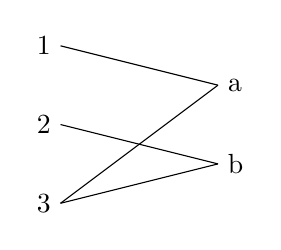
\begin{tikzpicture}[scale=1.0]
    \draw (1.0,1.0) node[left]{3};
    \draw (1.0,2.0) node[left]{2};
    \draw (1.0,3.0) node[left]{1};
    \draw (3.0,1.5) node[right]{b};
    \draw (3.0,2.5) node[right]{a};
    \draw (1.0,3.0) -- (3.0,2.5);
    \draw (1.0,2.0) -- (3.0,1.5);
    \draw (1.0,1.0) -- (3.0,2.5);
    \draw (1.0,1.0) -- (3.0,1.5);
  \end{tikzpicture}
  \caption{Darstellung Relation als Grafik}
  \label{abb:rel:Darstellung Relation als Grafik}
\end{center}
\end{figure}
\end{Unit}

%% -----------------------------------------------------------------------------
\begin{Unit}[Beispiel] 
  Es seien $P = \{p_1, p_2, p_3, p_4\}$ eine Menge von Produkten und $L = 
  \{l_1, l_2, l_3\}$ eine Menge von Lieferanten. Dann ist $P \times L$ das
  kartesische Produkt der Produkte und Lieferanten. Wenn der Lieferant $l_1$ 
  die Produkte $p_1$ und $p_2$, der Lieferant $l_2$ die Produkte $p_1, p_3$ 
  und $p_4$ und der Lieferant $l_3$ die Produkte $p_2$ und $p_4$ liefert, so 
  kann die Relation $\mathcal{R}$ \enquote{wird geliefert von} dargestellt 
  werden durch 
  \begin{align}
    \mathcal{R} = \{(p_1,l_1), (p_2,l_1), (p_1,l_2), (p_3,l_2), (p_4,l_2), 
      (p_2,l_3), (p_4,l_3)\}
  \end{align}
\end{Unit}

%% -----------------------------------------------------------------------------
\begin{Unit}[Beispiel]
  Es sei $M = \{A,B,C,D\}$ eine Menge von vier Orten. Die Relation 
  $\mathcal{R}$ der \emph{Ortsverbindungen} auf $M$ sei definiert durch die
  Eigenschaft, dass das Tupel $(X,Y)$ genau dann in der Relation enthalten 
  ist, wenn es eine Verbindung vom Ort $X$ zum Ort $Y$ gibt. Existiert eine 
  direkte Verbindung von Ort $X$ nach Ort $Y$, dann bedeutet das nicht, dass 
  es auch eine direkte Verbindung von Ort $Y$ zum Ort $X$ gibt. Es sei
  \begin{align}
    \mathcal{R} = \{ &(A,B), (B,A), (A,C), (C,D), \\
      & (D,A), (B,D), (D,B), (B,C), (C,B) \} \nonumber \ . 
  \end{align}
  Die Relation kann auch als Grafik dargestellt werden (siehe Abbildung
  \ref{abb:rel:Ortsverbindungen}). Hierbei wird durch einen gerichteten Pfeil 
  von $X$ nach $Y$ dargestellt, dass das Tupel $(X,Y)$ in der Relation ist, 
  dass   es somit eine direkte Verbindung von $X$ nach $Y$ gibt.

\begin{figure}[htbp]
\begin{center}
  \setlength{\unitlength}{1.0cm}
  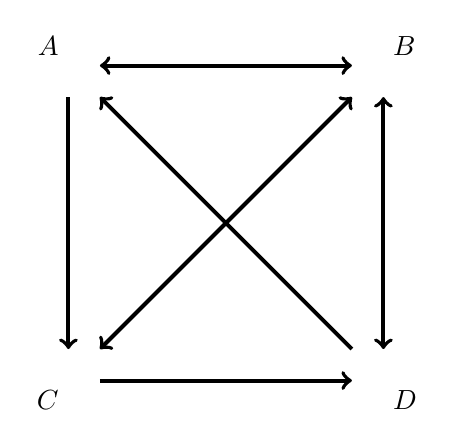
\begin{tikzpicture}[scale=2.0]
    \draw(1.0,3.0) node[above left]{$A$};
    \draw(3.0,3.0) node[above right]{$B$};
    \draw(1.0,1.0) node[below left]{$C$};
    \draw(3.0,1.0) node[below right]{$D$};
    \draw[line width=0.05cm, ->] (1.2,1.0) -- (2.8,1.0);
    \draw[line width=0.05cm, ->] (1.0,2.8) -- (1.0,1.2);
    \draw[line width=0.05cm, <->] (1.2,3.0) -- (2.8,3.0);
    \draw[line width=0.05cm, <->] (3.0,1.2) -- (3.0,2.8);
    \draw[line width=0.05cm, <->] (1.2,1.2) -- (2.8,2.8);
    \draw[line width=0.05cm, ->] (2.8,1.2) -- (1.2,2.8);
  \end{tikzpicture}
  \caption{Beispiel: Ortsverbindungen}
  \label{abb:rel:Ortsverbindungen}
\end{center}
\end{figure}
\end{Unit}

%% -----------------------------------------------------------------------------
\begin{Unit}[Beispiel] 
  Es sei $X = Y = \mg{R}$, dann ist
  \begin{align}
    K_2 := \{(x,y) \in \RR^2 \mid  (x^2\ +\ y^2\ =\ 4) \} 
  \end{align}
  eine Relation von $\RR^2$. Grafisch sind es die Punkte im 2-dimensionalen 
  Anschaungsraum, die auf einem Kreis mit Radius 2 um den Ursprung liegen.
\end{Unit}

%% -----------------------------------------------------------------------------
\begin{Unit}[Beispiel] 
  Es sei $X = Y = \NN$, dann sind
  \begin{align}
    \mathcal{R} := \{ (x,y) \in \NN^2 \mid (x \leq y) \}
  \end{align}
  und
  \begin{align}
    \mathcal{R} := \{ (x,y) \in \NN^2 \mid (x < y) \}
  \end{align}
  Relationen von $\NN^2$. Veranschaulichen Sie sich die Menge grafisch.
\end{Unit}

%% -----------------------------------------------------------------------------
\begin{Unit}[Beispiel] 
  Es sei $X = Y = \NN$, dann ist
  \begin{align}
    \mathcal{R}  := \{ (x,y) \in \NN^2 \mid (x - y = 1) \lor
      (y - x = 1) \} 
  \end{align} eine Relation von $\NN^2$.
\end{Unit}

%% -----------------------------------------------------------------------------
\begin{Unit}[Beispiel] 
  Es sei $M$ eine beliebige Menge und $X = Y = \mathcal{P}(M)$ die Potenzmenge 
  von $M$, dann ist
  \begin{align}
    T := \{ (U,V) \mid (U \subseteq M) \land (V \subseteq M) \land (U \subseteq 
      V) \} 
  \end{align}
  eine Relation von $\mathcal{P}(M)^2$.
\end{Unit}

%% -----------------------------------------------------------------------------
\begin{Unit}[Beispiel] 
  Es sei $X = Y = \ZZ$, dann ist für $n \in \NN$ 
  \begin{align}
    \mathcal{R}_n := \{ (x,y) \in \ZZ^2 \mid n|(x - y) \} 
  \end{align}
  eine Relation von $\ZZ^2$. Ein Tupel $(x,y)$ ist in der Relation, wenn die 
  Differenz der beiden Zahlen durch $n$ teilbar ist. 
  
  Für $n = 1$ ist $\mathcal{R}_1 = \ZZ^2$, also trivial. 
  
  Für $n = 2$ ist $\mathcal{R}_2$ die Menge der ganzzahligen 2-Tupel, für 
  welche die Differenz der beiden Zahlen durch 2 teilbar ist. So sind die 
  Tupel $(0,0)$, $(0,2)$, $(1,3)$, $(12,-6)$ Elemente der Relation, während 
  $(17,12)$ nicht zur Relation gehört. 
  
  Für $n = 5$ sind beispielsweise die Tupel $(0,0)$, $(0,5)$, $(0,10)$, 
  $(1,6)$, $(2,7)$, $(3,8)$, $(5,0)$ und $(17,12)$ in der Relation. Nicht in 
  der Relation sind beispielsweise $(0,1)$, $(0,2)$, $(0,3)$, $(0,4)$ und 
  $(12,8)$.

  Verdeutlichen Sie sich, welche Elemente in der Relation
  \begin{align}
    \mathcal{R}_n = \{ (x,y) \in \ZZ^2 \mid n|(x - y) \}
  \end{align}
  für $n = 1, 2, 3, 4, 5$ und $6$ enthalten sind.
\end{Unit}

%% -----------------------------------------------------------------------------
\begin{Unit}[Definition Inverse Relation]
Für die Relationen können einige spezielle Operationen definiert werden. Eine
davon ist die inverse Relation.

\begin{Definition}
  Es sei $\mathcal{R} \subseteq X \times Y$ eine binäre Relation.
  Die \Begriff{inverse Relation}\index{Relation, inverse}
  $\mathcal{R}^{-1}$ ist definiert durch
  \begin{align}
    \mathcal{R}^{-1} = \{ (y,x) \in Y \times X \mid (x,y) \in \mathcal{R} \} 
    \ .
  \end{align}
\end{Definition}

Ist $(x,y)$ eine Element aus $\mathcal{R} \subseteq X \times Y$, dann ist 
$(y,x)$ ein Element aus $\mathcal{R}^{-1} \subseteq Y \times X$.
\end{Unit}
\Translation{inverse Relation}{inverse relation}

%% -----------------------------------------------------------------------------
\begin{Unit}[Beispiel][Inverse Relation]
  Es sei $X = Y = \NN$ und $\mathcal{R} \subseteq X \times Y = \NN^2$. 
  Hierbei   sei $\mathcal{R}$ definiert durch
  \begin{align}
    \mathcal{R} = \{ (1,1), (1,2), (1,4), (2,3), (4,2)\} \ . 
  \end{align}
  Dann gilt
  \begin{align}
    \mathcal{R}^{-1} = \{ (1,1), (2,1), (4,1), (3,2), (2,4)\} \ . 
  \end{align}
\end{Unit}

%% -----------------------------------------------------------------------------
\begin{Unit}[Definition Komposition]
Eine weitere Operation ist die Komposition von Relationen.

\begin{Definition}
  Es seien $\mathcal{R} \subseteq X \times Y$ und $\mathcal{S} \subseteq Y 
  \times Z$ binäre Relationen. Die \Begriff{Komposition} $\mathcal{S} \circ 
  \mathcal{R}$ ist eine Relation zwischen $X$ und $Z$. Sie ist definiert 
  durch
  \begin{align}
    \mathcal{S} \circ \mathcal{R} = \{ (x,z) \in X \times Z \mid \exists y 
    \in Y : (x,y) \in \mathcal{R} \land (y,z) \in \mathcal{S} \} 
  \end{align}
\end{Definition}

Die Komposition $\mathcal{S} \circ \mathcal{R}$ beinhaltet somit die Tupel 
$(x,z) \in X \times Z$, für die es ein Element $y \in Y$ gibt, so dass sowohl 
$(x,y) \in \mathcal{R}$, als auch $(y,z) \in \mathcal{S}$ gelten. Die 
Schreibweise $\mathcal{S} \circ \mathcal{R}$ ist nicht einheitlich. Manchmal,
auch in früheren Versionen des Skripts, wurde es anders herum geschrieben.
\end{Unit}
\Translation{Komposition}{composition}

%% -----------------------------------------------------------------------------
\begin{Unit}[Beispiel Komposition]
  Es sei $X = Y = Z = \NN$, $\mathcal{R} \subseteq X \times Y = \NN^2$ und 
  $\mathcal{S} \subseteq Y \times Z = \NN^2$. Hierbei sei $\mathcal{R}$
  definiert durch
  \begin{align}
    \mathcal{R} = \{ (1,1), (1,2), (1,4), (2,3), (4,2)\}  
  \end{align}
  und $\mathcal{S}$ durch
  \begin{align}
    \mathcal{S} = \{ (1,3), (2,2), (1,4), (3,5)\} \ .  
  \end{align}
  Dann gilt
  \begin{align}
    \mathcal{S} \circ \mathcal{R} = \{ (1,3), (1,4), (1,2), (2,5), (4,2)\}
  \end{align} 
\end{Unit}

%% -----------------------------------------------------------------------------
\begin{Unit}[Beispiel Komposition]
  Es sei $X = Y = \NN$, $\mathcal{R} \subseteq X \times Y = \NN^2$. Hierbei 
  sei $\mathcal{R}$ definiert durch
  \begin{align}
    \mathcal{R} = \{ (1,1), (1,2), (1,4), (2,3), (4,2)\} \ .
  \end{align}
  Dann gilt
  \begin{align}
    \mathcal{R}^2 &= \mathcal{R} \circ \mathcal{R} = \{ (1,1), (1,2), (1,3), 
    (1,4), (4,3)\} \\
    \mathcal{R}^3 &= \mathcal{R}^2 \circ \mathcal{R} = \{ (1,1), (1,2), 
    (1,3), (1,4) \}
  \end{align} 
  Weiterhin gilt, hier im speziellen Fall, $\mathcal{R}^4$ = $\mathcal{R}^3$.
\end{Unit}

%%------------------------------------------------------------------------------

%%------------------------------------------------------------------------------
%% Abschnitt: Eigenschaften
%%------------------------------------------------------------------------------
\section{Eigenschaften}
\label{sec:Relationen:Eigenschaften}

%% -----------------------------------------------------------------------------
\begin{unit}
Für 2-stellige Relationen $\mathcal{R} \subseteq X \times Y$, mit beliebigen 
nicht leeren Mengen $X$ und $Y$ wird auch $x\mathcal{R}y$ statt $(x,y) \in
\mathcal{R}$ geschrieben. Im nachfolgenden werden hauptsächlich 2-stellige 
Relationen $\mathcal{R} \subseteq X \times X$, mit einer beliebigen Menge 
$X$, betrachtet. Es heißt dann auch Relation \textbf{auf} $X$
\index{Relation auf}. Im Nachfolgenden einige wichtige Eigenschaften von 
Relationen auf $X$.
\end{unit}

%% -----------------------------------------------------------------------------
\begin{Unit}[Definition reflexiv, irreflexiv]
Zuerst werden Beziehungen eines Elementes zu sich selbst betrachtet.
\begin{Definition}
  Es sei $X$ eine beliebige, nicht leere Menge. Eine Relation $\mathcal{R} 
  \subseteq X \times X$ heißt \Begriff{reflexiv}, falls für alle $x \in 
  X$, $(x, x) \in \mathcal{R}$
  \begin{align}
    \forall x \in X:\ (x, x) \in \mathcal{R}
  \end{align}
  gilt. Eine Relation $\mathcal{R} \subseteq X \times X$ heißt 
  \Begriff{irreflexiv}, falls für alle $x \in X$, $(x, x) \notin 
  \mathcal{R}$
  \begin{align}
    \forall x \in X:\ (x, x) \notin \mathcal{R}
  \end{align}
  gilt. 
\end{Definition}

Ist die Relation reflexiv, dann steht jedes Element in einer Beziehung zu sich
selbst. Ist die Relation irreflexiv, dann steht jedes Element nicht in einer
Beziehung zu sich.
\end{Unit}
\Translation{reflexiv}{reflexive}
\Translation{irreflexiv}{irreflexive}

%% -----------------------------------------------------------------------------
\begin{Unit}[Definition symmetrisch, asymmetrisch, antisymmetrisch]
Beziehun\-gen zwischen zwei Elemeneten werden nun betrachtet.
\begin{Definition}
  Es sei $X$ eine beliebige, nicht leere Menge. Eine Relation $\mathcal{R} 
  \subseteq X \times X$ heißt \Begriff{symmetrisch}, falls für alle 
  $x, y \in X$ aus $(x, y) \in \mathcal{R}$ folgt, dass auch $(y, x) \in 
  \mathcal{R}$ 
  \begin{align}
    \forall (x,y \in X)\ :\ (x, y) \in \mathcal{R} \rightarrow (y, x) \in 
      \mathcal{R}
  \end{align}
  gilt. Eine Relation $\mathcal{R} \subseteq X \times X$ heißt 
  \Begriff{asymmetrisch}, falls für alle $x, y \in X$ aus $(x, y) \in 
  \mathcal{R}$ folgt, dass $(y, x) \notin \mathcal{R}$
  \begin{align}
    \forall (x,y \in X)\ :\ (x, y) \in \mathcal{R} \rightarrow (y, x) \notin 
      \mathcal{R}
  \end{align} 
  gilt. Eine Relation $\mathcal{R} \subseteq X \times X$ heißt 
  \Begriff{antisymmetrisch}, falls für alle $x, y \in X$ aus $(x, y) \in 
  \mathcal{R}$ und $(y, x) \in \mathcal{R}$ folgt, dass dann $x\ =\ y$
  \begin{align}
    \forall (x, y \in X)\ :\ (x, y) \in \mathcal{R} \land (y, x) \in 
      \mathcal{R} \rightarrow\ (x = y)
  \end{align}
  gilt.
\end{Definition}
Wenn das Tupel $(x,y)$ in der Relation ist, dann ist das Tupel $(y,x)$ in der 
Relation, wenn die Relation symmetrisch ist. Bei einer asymmetrischen Relation
ist das Tupel $(y,x)$ nicht in der Relation. Bei einer antisymmetrischen 
Relation folgt aus der Tatsache, dass sowohl das Tupel $(x,y)$, als auch das 
Tupel $(y,x)$ in der Relation ist, dass dann $x$ und $y$ gleich sind.

Besonders zu beachten ist, dass die Eigenschaften symmetrisch und 
antisymmetrisch nicht die \enquote{Negation} zueinander sind. Das heißt eine
Relation die nicht symmetrisch ist, ist damit nicht automatisch
antisymmetrisch. Und eine Relation, die nicht antisymmetrisch ist, ist
nicht automatisch damit symmetrisch. Ebenso wenig ist eine Relation, die
nicht symmetrisch ist, asymmetrisch.
\end{Unit}
\Translation{symmetrisch}{symmetric}
\Translation{asymmetrisch}{asymmetric}
\Translation{antisymmetrisch}{antisymmetric}

%% -----------------------------------------------------------------------------
\begin{Unit}[Definition transitiv]
Nun wird eine Folge von Tupeln betrachtet.
\begin{Definition}
  Es sei $X$ eine beliebige, nicht leere Menge. Eine Relation $\mathcal{R} 
  \subseteq X \times X$ heißt \Begriff{transitiv}, falls für alle $x, y, z 
  \in X$ aus $(x, y) \in \mathcal{R}$ und $(y, z) \in \mathcal{R}$ folgt, 
  dass auch $(x, z) \in \mathcal{R}$ gilt:
  \begin{align}
    \forall (x, y, z \in X):\ (x, y) \in \mathcal{R} \land (y, z) \in
      \mathcal{R} \rightarrow\ (x, z) \in \mathcal{R}
  \end{align}
  gilt.
\end{Definition}
Wenn $(x,y)$ und $(y,z)$ aus der Relation sind, dann ist auch $(x,z)$ aus 
der Relation.
\end{Unit}
\Translation{transitiv}{transitive}

%% -----------------------------------------------------------------------------
\begin{Unit}[Definition vollständig, linear, konnex]
Ist es immer möglich, eine Beziehung zwischen zwei Elementen zu haben?
\begin{Definition}
  Es sei $X$ eine beliebige, nicht leere Menge. Eine Relation $\mathcal{R} 
  \subseteq X \times X$ heißt \Begriff{vollständig} oder 
  \Begriff{linear}, falls für alle $x, y \in X$ $(x, y) \in \mathcal{R}$ 
  oder $(y, x) \in \mathcal{R}$ gilt:
  \begin{align}
    \forall (x \in X)\ and\ (y \in X):\ (x, y) \in \mathcal{R} \lor (y, x)
      \in \mathcal{R} \ .
  \end{align}
  Sie heißt \Begriff{konnex}, wenn für alle $x, y \in X$ mit $x \not= y$ 
  gilt, dass $(x, y) \in \mathcal{R}$ oder $(y, x) \in \mathcal{R}$:
  \begin{align}
    \forall (x \in X)\ and\ (y \in X):\ x \not= y \Rightarrow (x, y) \in 
    \mathcal{R} \lor (y, x) \in \mathcal{R} \ .
  \end{align}
\end{Definition}
Mindestens eines der Paare $(x,y)$ und $(y,x)$ ist in der Relation. Wenn eine 
Relation vollständig ist, dann bedeutet dies, dass zu zwei Elementen $x$ und 
$y$ stets $(x,y)$ oder $(y,x)$ (oder auch beide) in der Relation sind.
\end{Unit}
\Translation{vollständig}{complete}
\Translation{linear}{linear}
\Translation{konnex}{connected}

%% -----------------------------------------------------------------------------
\begin{Unit}[Beispiel] 
  Es sei $X = Y = \NN$, dann ist $\mathcal{R} := \{ (x,y) \mid x \leq y) \}$ 
  eine Relation von $\NN^2$. Die Relation ist reflexiv, antisymmetrisch, 
  transitiv und vollständig.
\end{Unit}

%% -----------------------------------------------------------------------------
\begin{Unit}[Beispiel] 
  Es sei $X = Y = \NN$, dann ist $\mathcal{R} := \{ (x,y) \mid x < y) \}$ 
  eine   Relation von $\NN^2$. Die Relation ist irreflexiv, transitiv und 
  antisymmetrisch, jedoch nicht reflexiv oder symmetrisch.
\end{Unit}

%% -----------------------------------------------------------------------------
\begin{Unit}[Beispiel] 
  Es sei $X = Y = \RR$, dann ist $\mathcal{R} := \{ (x,y) \mid x \leq y) \}$ 
  eine Relation von $\RR^2$. Die Relation ist reflexiv, antisymmetrisch, 
  transitiv und vollständig.
\end{Unit}

%% -----------------------------------------------------------------------------
\begin{Unit}[Beispiel] 
  Es sei $X = Y = \RR$, dann ist $\mathcal{R} := \{ (x,y) \mid x^2 + y^2 = 4 \}$ 
  eine Relation von $\RR^2$. Die Relation ist symmetrisch.
\end{Unit}

%% -----------------------------------------------------------------------------
\begin{Unit}[Beispiel] 
  Es seien $X = Y = \ZZ$ und $n \in \NN$, dann ist $\mathcal{R} := \{ (x,y) \mid 
    n|(x - y) \}$ eine Relation von $\ZZ^2$. Die Relation ist reflexiv, 
    symmetrisch und transitiv.
\end{Unit}

%% -----------------------------------------------------------------------------
\begin{Unit}[Definition Äquivalenzrelation, Ordnungsrelation]
Die wichtigsten Relationen erfüllen gleichzeitig mehrere der Eigenschaften 
reflexiv, symmetrisch, antisymmetrisch, transitiv und voll\-stän\-dig.

\begin{Definition}
  Es seien $X$ eine beliebige, nicht leere Menge und $\mathcal{R} \subseteq X 
  \times X$ eine Relation auf $X$.
  \begin{enumerate}
    \item $\mathcal{R}$ heißt \Begriff{Äquivalenzrelation} auf $X$, falls
      sie reflexiv, transitiv und symmetrisch ist. In diesem Fall wird 
      $a \approx b$ anstelle von $(a, b) \in \mathcal{R}$ geschrieben und 
      \enquote{a ist äquivalent zu b} gesagt. 
    \item $\mathcal{R}$ heißt \Begriff{Ordnungsrelation} auf $X$, falls sie 
      reflexiv, transitiv und antisymmetrisch ist. In diesem Fall wird 
      $a \preceq b$ anstelle von $(a, b) \in \mathcal{R}$geschrieben und 
      \enquote{a ist kleiner gleich b} gesagt. 
    \item $\mathcal{R}$ heißt \Begriff{Präferenzrelation} auf $X$, falls 
      sie reflexiv, transitiv und voll\-ständig ist. In diesem Fall wird 
      $a \preceq b$ anstelle von $(a, b) \in \mathcal{R}$ geschrieben und 
      \enquote{a ist höchstens so gut wie b} gesagt.
  \end{enumerate}
\end{Definition}

Bevor die Äquivalenz- und Ordnungsrelationen genauer betrachten werden 
folgen nun einige Beispiele für solche Relationen.
\end{Unit}
\Translation{Äquivalenzrelation}{equivalence relation}
\Translation{Ordnungsrelation}{order relation}
\Translation{Präferenzrelation}{preference relation}

%% -----------------------------------------------------------------------------
\begin{Unit}[Beispiel] 
  Es sei $X = Y = \NN$, dann ist $\mathcal{R}_{\leq} := \{ (x,y) \mid x 
  \leq y) \}$ eine Relation von $\NN^2$. Die Relation ist reflexiv, 
  antisymmetrisch, transitiv und vollständig und daher eine (vollständige)
  Ordnungsrelation (auf $\NN$).
\end{Unit}

%% -----------------------------------------------------------------------------
\begin{Unit}[Beispiel] 
  Es sei $X = Y = \RR$, dann ist $\mathcal{R}_{\leq} := \{ (x,y) \mid x 
  \leq y) \}$ eine Relation von $\RR$. Die Relation ist reflexiv, 
  antisymmetrisch, transitiv und vollständig und daher eine (vollständige)
  Ordnungsrelation (auf $\RR$).
\end{Unit}

%% -----------------------------------------------------------------------------
\begin{Unit}[Beispiel] 
  Es sei $M$ eine beliebige, nicht leere Menge und $X = Y = \mathcal{P}(M)$ 
  die Potenzmenge von $M$, dann ist $\mathcal{R} := \{ (U,V) \mid 
  (U \subseteq V)\}$ eine Relation auf $\mathcal{P}(M)$. Die Relation ist 
  reflexiv, antisymmetrisch und transitiv und daher eine Ordnungsrelation 
  (auf $\mathcal{P}(M)$). Die  Relation ist jedoch nicht vollständig.
\end{Unit}

%% -----------------------------------------------------------------------------
\begin{Unit}[Beispiel] 
  Es sei $X = \RR$, dann wird durch $\mathcal{R} := \{ (x,y) \in \RR^2 
  \mid |x| \leq |y| \}$ eine Präferenzrelation auf $\RR$ definiert. Sie ist
  reflexiv, transitiv und vollständig, jedoch weder symmetrisch noch
  antisymmetrisch, daher ist es eine Präferenzrelation.
\end{Unit}

%% -----------------------------------------------------------------------------
\begin{Unit}[Beispiel] 
  Es sei $X$ eine Menge von Gütern. Jedem $x \in X$ sei ein Wert $u(x)$ 
  zugeordnet, der als Nutzen von $x$ interpretiert wird. Dann wird durch 
  $\mathcal{R} := \{ (x,y) \in X^2 \mid u(x) \leq u(y) \}$ eine
  Präferenzrelation auf $X$ definiert. Sie ist reflexiv, transitiv und 
  vollständig, jedoch weder symmetrisch noch antisymmetrisch, daher ist es 
  eine Präferenzrelation.
\end{Unit}

%%------------------------------------------------------------------------------
%% Abschnitt: Äquivalenzrelationen
%%------------------------------------------------------------------------------
\section{Äquivalenzrelationen}
\label{sec:Relationen:Aequivalenzrelationen}

%% -----------------------------------------------------------------------------
\begin{Unit}[Beispiel]
Eine Äquivalenzrelation ist eine Relation, die reflexiv, symmetrisch und 
transitiv ist. Dazu einige Beispiele.

\begin{enumerate}
\item 
  In der Geometrie ist die Parallelität von Geraden eine Äquivalenzralation 
  auf der Menge der Geraden.
\item
  Die Anzahl der Elemente einer Menge (Mächtigkeit) ist eine 
  Äquivalenzrelation auf der Menge der endlichen Mengen.
\end{enumerate}
\end{Unit}

%% -----------------------------------------------------------------------------
\begin{Unit}[Beispiel] 
  Es sei $X = \ZZ$, dann ist für $n \in \NN \backslash \{1\}$
  \begin{align}
    \mathcal{R}_n := \{ (x,y) \mid  (n|(x - y) \} \subseteq\ \ZZ^2
  \end{align}
  eine Relation. Die Relation ist reflexiv, symmetrisch und transitiv, daher 
  ist die Relation eine Äquivalenzrelation. Ist $(x, y) \in \mathcal{R}_n$ 
  dann wird auch $x \equiv y \modulo n$ oder $x \equiv_n y$ geschrieben und 
  \enquote{$x$ ist kongruent zu $y$ modulo $n$} gesagt. \\
  Sind $x$ und $y$ kongruent modulo $n$, dann besitzen $x$ und $y$ bei der 
  Division durch $n$ den selben Rest.

Für $n = 1$ wäre $\mathcal{R}_1 = \ZZ^2$. Daher ist dieses Beispiel einfach 
und wird im weiteren nicht vertieft.
\end{Unit}

%% -----------------------------------------------------------------------------
\begin{Unit}[Beispiel]
  Es sei $X = \NN$. Jedem $n \in \NN$ wird durch $q(n)$ die Quersumme 
  zugeordnet. Durch
  \begin{align}
    \mathcal{R} := \{ (x,y) \in \NN^2 \mid q(x) = q(y) \}
  \end{align}
  ist eine Äquivalenzrelation auf $\NN$ definiert wird.
\end{Unit}

%% -----------------------------------------------------------------------------
\begin{Unit}[Definition Äquivalenzklasse]
Die Elemente einer Menge, die bezüglich einer Äquivalenzrelation zueinander 
äquivalent sind bilden eine Teilmenge der Menge. Diese Teilmengen werden nun
genauer betrachtet.

\begin{Definition}
  Es sei $X$ eine beliebige Menge und $\mathcal{R} \subseteq X \times X$ eine 
  Äquivalenzrelation auf $X$. Für jedes $x \in X$ heißt die Menge
  \begin{align}
    [x] := \{ y \in X \mid y \approx x \}
  \end{align}
  die \Begriff{Äquivalenzklasse} von $x$.
\end{Definition}

Eine Äquivalenzrelation $[x]$ enthält somit all diejenigen Elemente der Menge, 
die zu $x$ äquivalent sind.
\end{Unit}
\Translation{Äquivalenzrelation}{equivalence relation}

%% -----------------------------------------------------------------------------
\begin{Unit}[Bemerkung]
Für Äquivalenzklassen gelten folgende Aussagen:

\begin{Bemerkung}
  Es sei $X$ eine beliebige Menge und $\mathcal{R} \subseteq X \times X$ eine 
  Äquivalenzrelation auf $X$, dann gelten:
  \begin{enumerate}
    \item Jede Äquivalenzklasse ist ungleich der leeren Menge. 
    \item Sind zwei Elemente $x$ und $y$ äquivalent, dann sind die 
      Äquivalenzklassen $[x]$ und $[y]$ von $x$ und $y$ identisch. 
    \item Jedes Element gehört zu genau einer Äquivalenzklasse.
    \item Je zwei Äquivalenzklassen sind entweder identisch oder disjunkt.
  \end{enumerate}
\end{Bemerkung}

Beweis:
\begin{enumerate}
  \item Da $x \in [x]$ gilt, ist eine Äquivalenzklasse nicht die leere Menge.
  \item Wenn $x \approx y$ gilt, dann gilt für ein $z \in X$:
    \begin{align}
      z \in [x] \leftrightarrow z \approx x \leftrightarrow z \approx y 
      \leftrightarrow z \in [y]
    \end{align}
    Die mittlere (Aussagen-)Äquivalenz gilt auf Grund der Transitivität der 
    Relation, da $x \approx y$ gilt. Damit wurde die Mengenidentität von 
    $[x]$ und $[y]$ gezeigt, da jedes Element von $[x]$ auch Element von 
    $[y]$ ist und umgekehrt. Also wurde die gegenseitige Teilmengenbeziehung
    gezeigt.
  \item Da $x \in [x]$, gehört $x$ mindestens zu einer Äquivalenzklasse. 
    Falls $x \in [y]$ und $x \in [z]$ gelten, dann folgt daraus, dass 
    $x \approx y$ und $x \approx z$ gilt. Auf Grund der Transitivität der 
    Relation ist dann $y \approx z$ und somit $[y] = [z]$. Damit gehört x zu 
    maximal einer und zu genau einer Äquivalenzklasse.
  \item Folgt direkt aus den obigen Aussagen.
\end{enumerate}\qed
\end{Unit}

%% -----------------------------------------------------------------------------
\begin{Unit}[Anmerkung]
Jede Äquivalenzrelation auf einer Menge $X$ zerlegt damit $X$ in paarweise
disjunkte, nicht leere Mengen, die Äquivalenzklassen. Es entsteht somit eine 
Klasseneinteilung. Genauso folgt aus einer Klasseneinteilung einer Menge eine 
Äquivalenzrelation, indem zwei Elemente genau dann in einer Äquivalenzklasse 
sind, wenn sie zur selben Klasse bezüglich der Klasseneinteilung gehören.
\end{Unit}

%% -----------------------------------------------------------------------------
\begin{Unit}[Definition Quotientenmenge]
Eine Äquivalenzrelation erzeugt eine neue Menge, die Menge der 
Äquivalenzklassen von $X$. Hierbei muss beachtet werden, dass die Elemente 
der Klasseneinteilung selber Mengen sind, nämlich die Äquivalenzklassen.

\begin{Definition}
  Es sei $X$ eine beliebige, nicht leere Menge und $\mathcal{R} \subseteq X 
  \times X$ eine Äquivalenzrelation auf $X$, dann heißt die Menge der
  Äquivalenzklassen von $X$ nach $\mathcal{R}$
  \begin{align}
    X / \mathcal{R} := \{ [x] \mid x \in X \}
  \end{align}
  die \Begriff{Quotientenmenge} von $X$ nach $\mathcal{R}$.\\
  Ein Element $y \in [x]$ heißt \Begriff{Repräsentant} der Klasse $[x]$.\\
  Eine Menge $V$ heißt \Begriff{vollständiges Repräsentantensystem}\index
  {Repräsentantensystem} von $X / \mathcal{R}$, wenn $V$ genau ein Element aus 
  jeder Klasse von $X / \mathcal{R}$ enthält.
\end{Definition}
\end{Unit}
\Translation{Quotientenmenge}{quotient set}
\Translation{Repräsentantensystem}{system of representatives}

%% -----------------------------------------------------------------------------
\begin{Unit}[Beispiel] 
  Die Geraden mit paralleler Richtung bilden die Äquivalenzklassen. Die 
  Parallelität von Geraden führt zum Begriff der Richtung.
\end{Unit}

%% -----------------------------------------------------------------------------
\begin{Unit}[Beispiel] 
  Die Mengen mit gleicher Elementanzahl bilden die Äquivalenzklassen auf der 
  Menge der endlichen Mengen. Die Mächtigkeit von Mengen führt zum Begriff 
  der Kardinalität.
\end{Unit}

%% -----------------------------------------------------------------------------
\begin{Unit}[Beispiel]
  Für jedes $n \in \NN\backslash \{1\}$ ist
  \begin{align}
    \mathcal{R}_n := \{ (x,y) \mid n|(x-y) \} \subseteq \ZZ^2
  \end{align}
  eine Relation. Ist $(x,y) \in \mathcal{R}_n$ dann wird auch $x \equiv y 
  \modulo n$ geschrieben und \enquote{$x$ ist kongruent zu $y$ modulo $n$} 
  gesagt. Für $n \in \NN \backslash \{1\}$ gibt es $n$ Repräsentanten der
  Quotientenmenge $\ZZ /
  \mathcal{R}_n$. Die Klassen seien $[0], [1], \ldots, [n-1]$. 
  Die Repräsentanten seien $0, 1, \ldots, n-1$. Durch
  \begin{align}
    [x] + [y]\ :=\ [x + y]
  \end{align}
  und
  \begin{align}
    [x] \cdot [y]\ := [x \cdot y]
  \end{align}
  wird auf der Quotientenmenge $\ZZ / \mathcal{R}_n  =:  \ZZ_n$ eine Addition 
  und eine Multiplikation definiert.
  \begin{enumerate}
    \item $\mathcal{R}_n$ ist eine Äquivalenzrelation.
    \item Für beliebiges $n \in \NN\backslash\{1\}$ und $i=0,1,\ldots,n-1$ 
    gilt
      \begin{align}
        [i] = \{z \in \ZZ \mid \exists x \in \ZZ : z = xn + i \}
      \end{align}
  \end{enumerate}
\end{Unit}

%% -----------------------------------------------------------------------------
\begin{Unit}[Beispiel]
  Es sei $M = \NN \times \NN$ die Menge der 2-Tupel mit natürlichen Zahlen. 
  Eine Relation $\mathcal{R}\ \subseteq M \times M$ sei definiert durch:
  \begin{align}
    \left( (a,b)\;,\;(c,d) \right) \in \mathcal{R}\ :\Leftrightarrow
      (a + d = b + c) \ .
  \end{align}
  Statt $\left( (a,b)\;,\;(c,d) \right) \in \mathcal{R}$ wird auch 
  $(a,b) \sim (c,d)$ geschrieben. 

  $\mathcal{R}$ ist eine Äquivalenzrelation auf $M = \NN \times \NN$. Die 
  Quotientenmenge $(\NN \times \NN) / \mathcal{R}$ oder $(\NN \times \NN) / 
  \sim$ ist äquivalent zu den ganzen Zahlen $\ZZ$.
\end{Unit}

%%------------------------------------------------------------------------------
%% Abschnitt: Ordnungsrelationen
%%------------------------------------------------------------------------------
\section{Ordnungsrelationen}
\label{sec:Relationen:Ordnungsrelationen}

%% -----------------------------------------------------------------------------
\begin{Unit}[Definition][teilweise geordnet, streng geordnet]
Es seien $M$ eine Menge und $\mathcal{R} \subseteq M \times M$ eine 
Ordnungsrelation. Eine Relation ist eine Ordnungsrelation, wenn sie reflexiv, 
transitiv und antisymmetrisch ist. Statt $(x,y) \in \mathcal{R}$ wird 
$x \preceq y$ geschrieben und \enquote{x ist kleiner (oder gleich) y} gesagt.

Wichtige Begriffe für Ordnungsrelationen werden eingeführt.

\begin{Definition}
  Eine binäre Relation $\preceq$ auf einer Menge $M$ heißt \Begriff
  {Ordnungsrelation}, \Begriff{teilweise Ordnung}\index{Ordnung, teilweise} 
  oder \Begriff{partielle Ordnung}\index{Ordnung, partielle}, wenn sie 
  reflexiv, antisymmetrisch und transitiv ist. Die Menge $M$ heißt dann 
  \Begriff{geordnete Menge}\index{Menge, geordnet} $(M,\preceq)$ oder 
  \Begriff{teilweise geordnete Menge}\index{Menge,teilweise geordnet}.\\
  Wenn eine Relation transitiv, jedoch nicht reflexiv ist, dann heißt die 
  Relation eine \Begriff{strenge Ordnungsrelation}\index{Ordnungsrelation, 
  strenge}. Eine Menge mit einer strengen Ordnungsrelation heißt \Begriff
  {streng geordnete Menge}\index{Menge, streng geordnet}.
\end{Definition}
\Translation{Ordnungsrelation}{partially ordered relation}
\Translation{partielle Ordnung}{partial order}
\Translation{strenge Ordnungsrelation}{strict partially order relation}
\Translation{streng geordnet}{strict partial order}

Für ein teilweise geordnete Menge wird auch kurz \Begriff
{tgo Menge}\index{Menge, tgo} oder \Begriff{poset} \enquote{partially 
ordered set} geschrieben.
\end{Unit}

%% -----------------------------------------------------------------------------
\begin{Unit}[Anmerkung]
Es sei $M$ eine Menge. Ist $\mathcal{R} \subseteq M \times M$ eine 
Ordnungsrelation, so kann daraus eine strenge Ordnungsrelation gebildet 
werden, indem die Relation $\mathcal{R} \backslash \mathcal{D} \subseteq 
M \times M$ gebildet wird, mit $\mathcal{D} := \{(x,x) \mid x \in M\}$. Es 
wird somit die \enquote{Diagonale} der Menge $M$ entfernt. Auf der anderen 
Seite kann aus einer strengen Ordnungsrelation eine Ordnungsrelation gebildet
werden, indem diese \enquote{Diagonale} zur Relation hinzugefügt wird. Daher 
wird zwischen einer Ordnungsrelation und einer strengen Ordnungsrelation 
hin- und herschalten.
\end{Unit}

%% -----------------------------------------------------------------------------
\begin{Unit}[Beispiel] 
  Die Mengen $(\NN, \leq)$, $(\ZZ, \leq)$, $(\QQ, \leq)$ und $(\RR, \leq)$ 
  mit der bekannten kleiner-gleich-Beziehung sind geordnete Mengen. \\
  Die Mengen $(\NN, <)$, $(\ZZ, <)$, $(\QQ, <)$, $(\RR, <)$ sind streng 
  geordnete Mengen.
\end{Unit}

%% -----------------------------------------------------------------------------
\begin{Unit}[Beispiel] 
  Es sei $M$ eine Menge, dann ist $(\mathcal{P}(M), \subseteq)$ eine geordnete 
  Menge. $(\mathcal{P}(M), \subset)$ ist eine streng geordnete Menge.
\end{Unit}

%% -----------------------------------------------------------------------------
\begin{Unit}[Beispiel] 
  Die Menge $(\NN, |)$ mit der Ordnungsrelation
  \begin{align}
    x \preceq y : \Leftrightarrow\ x|y
  \end{align}
  ist eine geordnete Menge. \\
  In diesem Beispiel ist die Ordnungsrelation durch die Teilbarkeit der 
  Zahlen bestimmt.
\end{Unit}

%% -----------------------------------------------------------------------------
\begin{Unit}[Beispiel]
  Für alle $n \in \NN$ gilt, dass $n|n$ gilt, daher ist die Relation reflexiv. 
  Es seien $n,m \in \NN$. Wenn $n|m$ und $m|n$ gilt, dann folgt daraus 
  $n = m$, somit ist die Relation antisymmetrisch. Wenn für $n,m,l \in \NN$ 
  gilt: $n|m$ und $m|l$, dann gilt auch $n|l$, und daher ist die Relation 
  transitiv. Somit ist die Relation insgesamt eine Ordnungsrelation.
\end{Unit}

%% -----------------------------------------------------------------------------
\begin{Unit}[Definition linear geordnet]
Die reellen Zahlen können auf einem Zahlenstrahl angeordnet werden. Gilt diese
Eigenschaft allgemeiner?

\begin{Definition}
  Eine Ordnungsrelation $\preceq$ auf einer Menge $M$ heißt \Begriff{total 
  geordnet}\index{geordnet, total}, \Begriff{konnex} oder \Begriff
  {linear geordnet}\index{geordnet, linear}, wenn für alle Elemente $x$, $y$ 
  der Menge $M$ $x \preceq y$ oder $y \preceq x$ gilt.
  \begin{align}
    (M, \preceq) \text{ linear geordnet } :\Leftrightarrow \forall 
    (x, y \in M): (x \preceq y) \lor (y \preceq x) \ .
  \end{align}
\end{Definition}
\Translation{linear geordnet}{linear ordered}

Bei einer total geordneten Menge verwendet wird oftmals auch das Symbol 
$\leq$ statt $\preceq$ verwendet. Damit wird die die Nähe zur totalen
Ordnung auf den Zahlenmengen $\NN$, $\ZZ$, $\QQ$ und $\RR$ verdeutlicht.

Bei einer linear geordneten Menge können die Elemente der Menge linear
angeordnet werden. Es kann für zwei Elemente der Menge stets angegeben werden, 
welche von beiden Zahlen kleiner ist.
\end{Unit}

%% -----------------------------------------------------------------------------
\begin{Unit}[Beispiel] 
  $(\NN, \leq)$, $(\ZZ, \leq)$, $(\QQ, \leq)$ und $(\RR, \leq)$ sind linear 
  geordnete Mengen.
\end{Unit}

%% -----------------------------------------------------------------------------
\begin{Unit}[Beispiel] 
  Es sei $M$ eine Menge, dann ist $(\mathcal{P}(M), \subseteq)$ keine linear 
  geordnete Menge.
\end{Unit}

%% -----------------------------------------------------------------------------
\begin{Unit}[Beispiel] 
  $(\NN, |)$ ist keine linear geordnete Menge.
\end{Unit}

%% -----------------------------------------------------------------------------
\begin{Unit}[Definition Ordnungsdiagramme]
Ordnungsstrukturen endlicher Mengen $(M, \preceq)$ lassen sich in einfachen 
Fällen übersichtlich in einem Diagramm darstellen. Diese Diagramme heißen
\Begriff{Ordnungsdiagramm} oder \Begriff{Hasse-Diagramm}, benannt nach 
dem deutschen Mathematiker Helmut Hasse (1898 - 1979)\index[names]{Hasse, 
Helmut}\footnote{\url{https://de.wikipedia.org/wiki/Helmut_Hasse}}. 
Jedem Element der Menge wird ein Punkt der Zeichenebene zugeordnet. Ist $a 
\preceq b$, so wird ein Pfeil von $a$ nach $b$ gezeichnet. Es kann vereinbart 
werden, dass ein Element $b$ oberhalb eines Elements $a$ gezeichnet wird, 
wenn $a \preceq b$ ist. Darüber hinaus werden $a$ und $b$ einfach verbunden. 
Ein Pfeil ist nicht notwendig, da durch die Anordnung \enquote{unten - oben} 
die Pfeilrichtung entnommen werden kann. Um die Anzahl der Linien zu 
reduzieren, werden keine Verbindungen eines Elements mit sich selbst 
gezeichnet, das heißt, dass die reflexive Eigenschaft nicht dargestellt wird.
Darüber hinaus wird $a$ nicht mit $b$ verbunden, wenn $b$ auch über andere 
Punkte mit $a$ verbunden ist, das heißt, die transitive Eigenschaft wird 
nicht dargestellt.
\end{Unit}
\Translation{Ordnungsdiagramm}{Hasse diagram}

%% -----------------------------------------------------------------------------
\begin{Unit}[Beispiel]
  Es sei $M = \{ n \in \NN \mid 1 < n < 10 \}$ und $x \preceq y 
  :\Leftrightarrow x|y$. Dann kann die Ordnungsrelation folgendermaßen 
  grafisch mit Hilfe eines Ordnungs- oder Hasse-Diagramm dargestellt werden 
  (siehe Abbildung \ref{abb:rel:Beispiel: Ordnungsrelation}).

\begin{figure}[htbp]
\begin{center}
  \setlength{\unitlength}{1.0cm}
  \begin{tikzpicture}[scale=1.0]
    \draw (1.0,1.0) node[below]{$2$};
    \draw (1.0,3.0) node[above]{$4$};
    \draw (1.0,5.0) node[above]{$8$};
    \draw (2.0,4.0) node[above]{$6$};
    \draw (3.0,2.0) node[below]{$3$};
    \draw (3.0,5.0) node[above]{$9$};
    \draw (4.5,3.0) node[below]{$5$};
    \draw (6.0,4.0) node[below]{$7$};
    \draw (1.0,1.0) -- (1.0,3.0);
    \draw (1.0,3.8) -- (1.0,5.0);
    \draw (1.0,1.0) -- (2.0,4.0);
    \draw (3.0,2.0) -- (2.0,4.0);
    \draw (3.0,2.0) -- (3.0,5.0);
  \end{tikzpicture}
  \caption{Beispiel: Ordnungsrelation}
  \label{abb:rel:Beispiel: Ordnungsrelation}
\end{center}
\end{figure}
\end{Unit}

%% -----------------------------------------------------------------------------
\begin{Unit}[Beispiel]

\begin{figure}[htbp]
\begin{center}
  \setlength{\unitlength}{1.0cm}
  \begin{tikzpicture}[scale=1.0]
    \draw (1.0,1.0) node[below]{$2$};
    \draw (1.0,3.0) node[above]{$4$};
    \draw (2.0,4.0) node[below]{$6$};
    \draw (2.0,6.0) node[above]{$12$};
    \draw (3.0,2.0) node[below]{$3$};
    \draw (4.5,3.0) node[below]{$5$};
    \draw (4.5,5.0) node[above]{$25$};
    \draw (6.0,4.0) node[below]{$7$};
    \draw (4.5,3.0) -- (4.5,5.0);  % 5 -- 25
    \draw (1.0,1.0) -- (2.0,3.4);  % 2 -- 6
    \draw (1.0,1.0) -- (1.0,3.0);  % 2 -- 4
    \draw (2.0,4.0) -- (2.0,6.0);  % 6 -- 12
    \draw (1.0,3.8) -- (2.0,6.0);  % 4 -- 12
    \draw (3.0,2.0) -- (2.0,3.4);  % 3 -- 6
  \end{tikzpicture}
  \caption{Beispiel: maximale und minimale Elemente}
  \label{abb:rel:Beispiel: maximale und minimale Elemente}
\end{center}
\end{figure}

\label{bsp:Relationen:Ordnungsrelation}
  Es sei $M = \{2, 3, 4, 5, 6, 7, 12, 25\}$ mit der Ordnungsrelation $a \preceq 
  b :\Leftrightarrow a|b$. Das Ordnungsdiagramm hat folgendes Aussehen (siehe 
  Abbildung \ref{abb:rel:Beispiel: maximale und minimale Elemente}) In diesem 
  Beispiel gibt es kein Element, das größer als 12, 25 oder 7 ist. Wird die 
  Menge auf die Element $\{2, 3, 4, 6, 12\}$ eingeschränkt, dann ist die 12 
  sogar größer als jedes andere Element der Menge. Dies führt zu Definitionen 
  von ausgezeichneten Elementen einer geordneten Menge.
\end{Unit}

%% -----------------------------------------------------------------------------
\begin{Unit}[Definition maximales Element, größtes Element]
Die Elemente im vorherigen Beispiel werden nun klar definiert.
  
\begin{Definition}
  Es sei $(M,\preceq)$ eine geordnete Menge. Ein Element $m$ aus $M$ heißt
  \Begriff{maximales Element}\index{Element, maximales} von $M$ ($m = 
  maxEl(M))$, wenn es kein Element gibt, das größer als $m$ ist:
  \begin{align}
    m = maxEl(M) :\Leftrightarrow (m \in M) \land [\forall (x \in M): m 
      \preceq x \rightarrow x = m] \ .
  \end{align} 
  Ein Element $g$ aus $M$ heißt \Begriff{größtes Element}\index{Element, 
  größtes} oder \Begriff{Maximum} von $M$ ($g = grEl(M))$, wenn $g$ größer 
  als jedes andere Element von $M$ ist:
  \begin{align}
    g = grEl(M) :\Leftrightarrow (g \in M) \land \forall (x \in M): 
    x \preceq g \ .
  \end{align} 
\end{Definition}
\Translation{maximales Element}{maximal element}
\Translation{größtes Element}{greatest element}

Für ein maximales Element gibt es keine Elemente in der Menge, die größer 
sind als dieses maximale Element. Ein größtes Element ist größer als jedes 
andere Element. Das ist ein kleiner, aber entscheidender Unterschied, der zu
beachten ist. Eine Menge kann durchaus mehrere maximale Element haben. Wenn 
ein größtes Element existiert, dann ist dieses eindeutig.
\end{Unit}

%% -----------------------------------------------------------------------------
\begin{Unit}[Definition minimales Element, kleinstes Element]
Nun die Elemente, die in der Ordnung unten stehen.
  
\begin{Definition}
  Es sei $(M,\preceq)$ eine geordnete Menge. Ein Element $m$ aus $M$ heißt 
  \Begriff{minimales Element}\index{Element, minimales} von $M$ ($m = 
  minEl(M)$), wenn es kein Element gibt, das kleiner als $m$ ist:
  \begin{align}
    m = minEl(M) :\Leftrightarrow (m \in M) \land [\forall (x \in M): 
    x \preceq m 
      \rightarrow x = m] \ .
  \end{align}
  Ein Element $k$ aus $M$ heißt \Begriff{kleinstes Element}\index{Element, 
  kleinstes} oder \Begriff{Minimum} von $M$ ($k = klEl(M)$), wenn $k$ 
  kleiner als jedes andere Element von $M$ ist:
  \begin{align}
    k = klEl(M) :\Leftrightarrow (k \in M) \land \forall(x \in M): 
    k \preceq x \ .
  \end{align}
\end{Definition}
\Translation{minimales Element}{minimal element}
\Translation{kleinstes Element}{least element}

Für ein minimales Element gibt es keine Elemente in der Menge, die kleiner 
sind als dieses minimale Element. Ein kleinstes Element ist kleiner als 
jedes andere Element. Das ist ein kleiner, aber entscheidender Unterschied, 
der zu beachten ist. Eine Menge kann durchaus mehrere minimale Element haben. 
Wenn ein kleinstes Element existiert, dann ist dieses eindeutig.
\end{Unit}

%% -----------------------------------------------------------------------------
\begin{Unit}[Beispiel] 
  Im Beispiel \ref{bsp:Relationen:Ordnungsrelation} sind 12, 25 und 7 
  maximale Elemente, die Zahlen 2, 3, 5 und 7 sind minimale Elemente. Es gibt 
  kein größtes oder kleinstes Element. Ein Element kann zugleich maximales und
  minimales Element sein. Für die Teilmenge {2, 3, 4, 6, 12} ist 12 ein 
  größtes Element. Ein größtes Element einer Menge muss nicht existieren. Genau
  sowenig ein kleinstes Element.
\end{Unit}

%% -----------------------------------------------------------------------------
\begin{Unit}[Beispiel]
  \label{bsp:Relationen:Wurzel2}
  Es sei
  \begin{align}
    F := \{x \in \QQ \mid x = 1 - \frac{1}{n}, n \in \NN \}
  \end{align}
  eine Teilmenge der geordneten Menge $(\QQ, \leq)$. Alle Elemente der Menge 
  sind kleiner 2 oder auch kleiner 3/2 oder auch kleiner 1. Somit gibt es 
  Element aus der Obermenge $\QQ$ von $F$, die eine obere Schranke für die 
  Elemente der Menge von $F$ bilden.
\end{Unit}

%% -----------------------------------------------------------------------------
\begin{Unit}[Definition Schranke, beschränkt]
Dies führt zu folgenden Definitionen.

\begin{Definition}
  Es sei $(M,\preceq)$ eine geordnete Menge und $T$ eine Teilmenge von $M$ 
  mit   der selben Ordnungsrelation. Ein Element $o$ aus $M$ heißt 
  \Begriff{obere Schranke} von $T$ ($o\ =\ obSch(T)$), wenn alle Elemente von 
  $T$ kleiner oder gleich $o$ sind
  \begin{align}
    o = obSch(T) :\Leftrightarrow  (o \in M) \land \forall (x \in T):
      x \preceq o \ .
  \end{align}
  Existiert eine obere Schranke für eine Menge $T$, so heißt die Menge 
  \Begriff{nach oben beschränkt}\index{beschränkt, nach oben}. \\ 
  Ein Element $u$ aus $M$ heißt \Begriff{untere Schranke}\index{Schranke, 
  untere} von $T$ ($u = untSch(T)$), wenn alle Elemente von $T$ größer oder 
  gleich $u$ sind
  \begin{align}
    u = untSch(T) :\Leftrightarrow (u \in M) \land \forall (x \in T): 
    u \preceq x \ .
  \end{align}
  Existiert eine untere Schranke für eine Menge $T$, so heißt die Menge 
  \Begriff{nach unten beschränkt}\index{beschränkt, nach unten}.
\end{Definition}
\Translation{Schranke}{bound}
\Translation{beschränkt}{bounded}
\Translation{obere Schranke}{upper bound}
\Translation{untereSchranke}{lower bound}

Eine obere oder untere Schranke einer Menge $T$ muss nicht in der Menge $T$ 
selbst enthalten sein, sie können in einer Obermenge existieren. Wenn eine 
Menge $T$ ein größtes oder ein kleinstes Element hat, dann ist dieses Element 
auch zugleich eine obere oder untere Schranke für die Menge $M$.
\end{Unit}

%% -----------------------------------------------------------------------------
\begin{Unit}[Beispiel]
  Für die obige Menge $F$ (siehe Beispiel \ref{bsp:Relationen:Wurzel2}) 
  sei $S$ die Menge der oberen Schranken. Es stellt sich die Frage nach 
  dem kleinsten Element dieser Menge. In diesem Beispiel ist 1 das kleinste 
  Element der oberen Schranken. Die 1 ist nicht in der Menge $F$ enthalten, 
  jedoch in der Obermenge $\QQ$.
\end{Unit}

%% -----------------------------------------------------------------------------
\begin{Unit}[Definition Grenze, Supremum, Infimum]
\ 

\begin{Definition}
  Ein Element $o$ aus $M$ heißt \Begriff{obere Grenze}\index{Grenze, obere} 
  von $T$ ($o = obGr(T)$), wenn $o$ das kleinste Element der Menge der oberen 
  Schranken von $T$ ist. Das Element $o$ heißt dann auch \Begriff{Supremum} 
  von $T$:
  \begin{align}
    o = obGr(T) :\Leftrightarrow (o \in M) \land o = klEl(S) 
  \end{align}
  mit $S = \{s \mid s = obSch(M) \}$.

  Ein Element $u$ aus $M$ heißt \Begriff{untere Grenze}\index{Grenze, 
  untere} von $T$ ($u = untGr(T)$), wenn $u$ das größte Element der Menge der 
  unteren Schranken von $T$ ist. Das Element $u$ heißt dann auch \Begriff
  {Infimum} von $T$:
  \begin{align}
    u = untGr(T) :\Leftrightarrow (u \in M) \land u = grEl(S) 
  \end{align}
  mit $S = \{s \mid s = untSch(M)\}$.
\end{Definition}
\Translation{obere Grenze}{supremum}
\Translation{Supremum}{supremum}
\Translation{untere Grenze}{infimum}
\Translation{Infimum}{infimum}

Eine obere oder untere Grenze muss nicht immer existieren. 
\end{Unit}

%% -----------------------------------------------------------------------------
\begin{Unit}[Beispiel]
  Sei nun
  \begin{align}
    W := \{x \in \QQ \mid x^2 \leq 2 \} \subseteq \QQ \ .
  \end{align}
  Die Menge $W$ ist nach oben beschränkt, denn beispielsweise 2; 1,5 oder 
  1,42 sind obere Schranken. Es gibt jedoch keine obere Grenze von $W$ in 
  $\QQ$, da $\sqrt{2}$ keine rationale Zahl ist. Erst wenn nicht $\QQ$, 
  sondern $\RR$ als Obermenge betrachtet wird, hat die Menge $W$ eine obere 
  Grenze.
\end{Unit}

%% -----------------------------------------------------------------------------
\begin{Unit}[Beispiel]
  Es sei $A := \{t \in \mg{N}\ |\ (t|36)\ and (t < 15)\}$ mit der 
  Ordnungsstruktur, die durch $a \leq b :\Leftrightarrow a|b$ definiert ist. 
  Die Elemente der Menge $A$ sind $A = \{1, 2, 3, 4, 6, 9, 12\}$. Das 
  Ordnungsdiagramm ist in Abbildung 
  \ref{abb:rel:Ordnungsrelation Teiler von 36} zu sehen.

\begin{figure}[htbp]
\begin{center}
  \setlength{\unitlength}{1.0cm}
  \begin{tikzpicture}[scale=1.5]
    \draw (0.50,2.50) node[below]{$4$};
    \draw (1.50,1.50) node[below]{$2$};
    \draw (1.50,3.50) node[below]{$12$};
    \draw (2.50,0.50) node[below]{$1$};
    \draw (2.50,2.50) node[below]{$6$};
    \draw (3.50,1.50) node[below]{$3$};
    \draw (4.50,2.50) node[below]{$9$};
    \draw (1.30,2.90) -- (0.70,2.30);
    \draw (2.30,1.90) -- (1.70,1.30);
    \draw (3.30,0.90) -- (2.70,0.30);
    \draw (4.30,1.90) -- (3.70,1.30);
    \draw (0.70,1.90) -- (1.30,1.30);
    \draw (1.70,0.90) -- (2.30,0.30);
    \draw (1.70,2.90) -- (2.30,2.30);
    \draw (2.70,1.90) -- (3.30,1.30);
  \end{tikzpicture}
  \caption{Ordnungsrelation Teiler von 36}
  \label{abb:rel:Ordnungsrelation Teiler von 36}
\end{center}
\end{figure}

  Die $9$ und die $12$ sind maximale Elemente, denn es gibt keine Elemente in 
  der Menge, die größer sind. Die $6$ hingegen ist kein maximales Element, da 
  die $12$ größer als die $6$ ist. Ein größtes Element existiert nicht, denn die 
  $12$ ist gemäß der Ordnungsstruktur nicht größer als $9$, da die $9$ kein 
  Teiler der $12$ ist. In der Obermenge der natürlichen Zahlen gibt es 
  verschiedene obere Schranken bezüglich der Ordnungsstruktur, zum Beispiel die 
  $36$ oder auch die $72$. Die $18$ ist keine obere Schranke, denn die $12$ ist 
  kein Teiler der $18$, also ist die $18$ nicht größer als jedes Element der 
  Menge. Das Supremum ist die $36$.

  Die $1$ ist minimales Element, kleinstes Element und Infimum der Menge.
\end{Unit}

%%% =============================================================================
%% Mathematische Grundlagen - Grundbegriffe
%% Kapitel 06 - Abbildungen und Funktionen
%% Autor: Andreas Zeh-Marschke
%% Datum: 2025-03-31
%% =============================================================================

\chapter{Abbildungen und Funktionen}
\label{cha:Gdl-K06-Abbildungen}

%% -----------------------------------------------------------------------------
%\begin{unit}
Eine spezielle Relation ist die Abbildung. Auf Grund der Wichtigkeit für den 
gesamten Bereich der Mathematik, werden Abbildungen genauer betrachtet. Nach 
der Definition von \textbf{Abbildungen} (Abschnitt 
\ref{sec:Abbildungen:Definition}) werden \textbf{Eigenschaften} von
Abbildungen (siehe Abschnitt \ref{sec:Abbildungen:Eigenschaften}) erläutert. 
Im Abschnitt \ref{sec:Abbildungen:Mengen von Abbildungen} werden kurz Mengen 
von Abbildungen betrachtet.
%\end{unit}

%%------------------------------------------------------------------------------
%% Abschnitt: Definition von Abbildungen
%%------------------------------------------------------------------------------
\section{Definition von Abbildungen}
\label{sec:Abbildungen:Definition}

%% -----------------------------------------------------------------------------
\begin{Unit}[Definition Abbildung]
Gleich die einfache Definition einer Abbildung.

\begin{Definition}
  Es seien $X$ und $Y$ zwei beliebige, nicht leere Mengen und $f \subseteq X 
  \times Y$ eine Vorschrift, die jedem Element von $X$ genau ein Element aus 
  $Y$ zuordnet:
  \begin{align}
    \forall x \in X\ \exists^1 y \in Y\ : (x, y) \in f \ .
  \end{align}
  Das Tripel $(f,X,Y)$ oder kurz $f$ heißt \Begriff{Abbildung} von $X$ nach 
  $Y$. Dafür wird auch 
  \begin{align}
    f:X \rightarrow Y\ ,\ x \mapsto f(x) = y 
  \end{align}
  geschrieben.
  Die Menge $X$ heißt der \Begriff{Definitionsbereich} von $f$. Die Menge 
  $Y$ heißt der \Begriff{Wertebereich} von $f$. Die Menge 
  \begin{align}
    f(X) := \{y \in Y \mid \exists x \in X: f(x) = y\}
  \end{align} 
  heißt \Begriff{Bild} von $f$, und die Menge 
  \begin{align}
    graph(f) := \{(x, f(x)) \mid x \in X\}
  \end{align} heißt \Begriff{Graph} von $f$.
\end{Definition}
\Translation{Abbildung}{mapping}
\Translation{Definitionsbereich}{domain}
\Translation{Wertebereich}{codomain}
\Translation{Graph}{graph}

\begin{figure}[htbp]
\begin{center}
  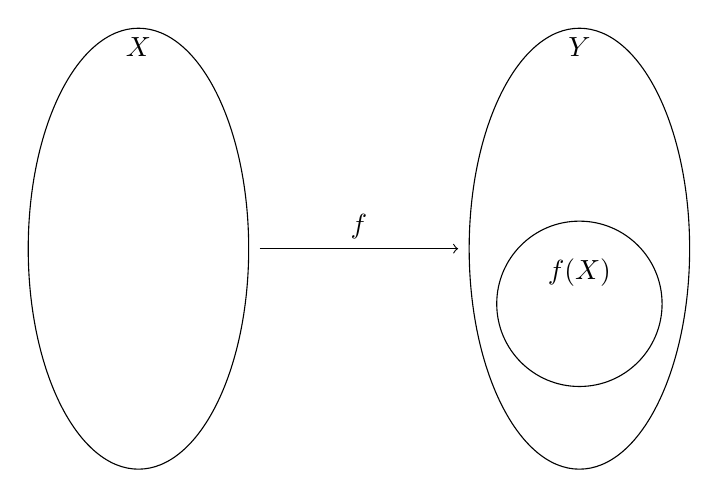
\begin{tikzpicture}[scale=0.7]
    \draw (-4.0,0.0) ellipse (2.0 and 4.0);
    \draw (-4.0,4.0) node[below]{$X$};
    \draw (4.0,0.0) ellipse (2.0 and 4.0);
    \draw (4.0,4.0) node[below]{$Y$};
    \draw (4.0,-1.0) circle (1.5);
    \draw (4.0,0.0) node[below]{$f(X)$};
    \draw[->] (-1.8,0.0) -- (1.8,0.0);
    \draw (0.0,0.0) node[above]{$f$};
  \end{tikzpicture}
  \caption{Abbildung}
  \label{abb:abb:Abbildung}
\end{center}
\end{figure}

Auf Grund der Eigenschaft $f \subseteq X \times Y$ ist $f$ eine Relation von 
$X \times Y$. Die zusätzliche Eigenschaft bedeutet, dass es für jedes Element 
von $x \in X$ genau ein Element $y \in Y$ gibt, so dass $(x,y) \in f$ ist. Es 
wird zwischen der Abbildung $f$ und dem Wert $f(x)$ der Abbildung $f$ an der 
Stelle $x$ unterschieden. In der Abbildung \ref{abb:abb:Abbildung} ist die 
Abbildung grafisch dargestellt.

Das Bild von $f$ ist eine Teilmenge von $Y$ $(f(X) \subseteq Y)$, der Graph 
von $f$ ist eine Teilmenge des kartesischen Produktes von $X$ und $Y$ 
$(graph(f) \subseteq X \times Y)$.
\end{Unit} 

%% -----------------------------------------------------------------------------
\begin{Unit}[Definition Gleichheit]
Wann sind zwei Abbildung gleich?

\begin{Definition}
Zwei Abbildungen $f: X \rightarrow Y$ und $g: X \rightarrow Y$ heißen
\Begriff{gleich}, wenn $f(x) = g(x)$ für alle $x \in X$ gilt.
\begin{align}
   f = g :\Leftrightarrow \forall x \in X: f(x) = g(x) \ .
\end{align}
\end{Definition}
\Translation{Gleichheit}{equality}

Hierbei ist auch wichtig, dass die Definitionsbereiche und die Wertebereiche
identisch sind.
\end{Unit} 

%% -----------------------------------------------------------------------------
\begin{Unit}[Beispiel] 
Die Abbildung, die einer natürlichen Zahl $n$ seinen Nachfolger zuordnet.
\begin{align}
  f: \NN \rightarrow \NN,\ n \mapsto f(n) = n + 1
\end{align}
$f(\NN) = \NN \backslash \{1\}$
\end{Unit}

%% -----------------------------------------------------------------------------
\begin{Unit}[Beispiel] 
Die Abbildung, die jeder natürlichen Zahl sein Doppeltes zuordnet.
\begin{align}
  f: \NN \rightarrow \NN,\ n \mapsto f(n) = 2n
\end{align}
$f(\NN) = \{2, 4, 6, 8, \ldots \}$
\end{Unit}

%% -----------------------------------------------------------------------------
\begin{Unit}[Beispiel] 
Die Abbildung, die jeder ganzen Zahl $z$ seinen Nachfolger zuordnet.
\begin{align}
  f: \ZZ \rightarrow \ZZ,\ z \mapsto f(z) = z + 1
\end{align}
$f(\ZZ) = \ZZ$
\end{Unit}

%% -----------------------------------------------------------------------------
\begin{Unit}[Beispiel] 
Die Abbildung, die einer geraden natürlichen Zahl den halben Wert zuordnet.
Den ungeraden natürlichen Zahlen wird eine negative Zahl zugeordnet.
\begin{align}
  f: \NN \rightarrow \ZZ, n \mapsto f(n) := 
  \begin{cases} 
    n/2      & \text{ falls }n{\ gerade } \\ 
    -(n-1)/2 & \text{ falls }n{\ ungerade } \ .
  \end{cases}
\end{align}
Es ist eine Abbildung von den natürlichen Zahlen in die Menge der ganzen 
Zahlen. Hierbei gibt es für jede ganze Zahl $z$ eine natürliche Zahl $n$, so
dass $f(n) = z$ ist. Somit gilt hier $f(\NN) = \ZZ$.
\end{Unit}

%% -----------------------------------------------------------------------------
\begin{Unit}[Beispiel] 
Die Abbildung, die jeder reellen Zahl das Quadrat der Zahl zuordnet.
\begin{align}
  f: \RR \rightarrow \RR, x \mapsto f(x) = x^2 \ .
\end{align}
Der Wertebereich sind die positiven reellen Zahlen, inklusive der $0$, es 
gilt also $f(\RR) = \RR^+_0$.
\end{Unit}

%% -----------------------------------------------------------------------------
\begin{Unit}[Beispiel] 
  \begin{align}
    f: \RR \rightarrow \RR, x \mapsto f(x) = \sqrt{x}
  \end{align}
  ist keine Abbildung, da nicht jedem $x \in \RR$ genau ein Wert zugewiesen 
  werden kann, da zum Einem die Wurzel von negativen Zahlen in $\RR$ nicht 
  definiert ist, und zum Anderen für positive Werte von $x \in \RR$ die 
  Wurzel zwei Lösungen hat, die positive und die negative Wurzel. Wird die 
  Vorschrift auf positive Werte eingeschränkt: $f:\RR^+_0 \rightarrow 
  \RR^+_0, x \mapsto f(x) = +\sqrt{x}$ dann entsteht eine Abbildung, mit 
  $f(\RR^+_0) = \RR^+_0$.
  
  Es ist die Regel, dass die Wurzel aus einer Zahl immer positiv ist. Daher
  gilt $\sqrt{x^2} = |x|$.
\end{Unit}

%% -----------------------------------------------------------------------------
\begin{Unit}[Beispiel] 
  Es sei $X$ eine Menge von Gütern, durch $u: X \rightarrow \RR, x \mapsto 
  u(x)$, wobei $u(x)$ der Nutzen des Gutes $x$ darstellt, wird eine Abbildung 
  definiert.
\end{Unit}

%% -----------------------------------------------------------------------------
\begin{Unit}[Beispiel]  
  Es sei $M$ eine (endliche) Menge und $\mathcal{P}(M)$ die Potenzmenge von 
  $M$, dann wird durch
  \begin{align}
    f: \mathcal{P}(M) \rightarrow \NN_0, T \mapsto f(T) := |T|
  \end{align}
  eine Abbildung definiert. Die Abbildung ordnet jeder Menge die Anzahl der 
  Elemente der Menge zu.
\end{Unit}

%% -----------------------------------------------------------------------------
\begin{Unit}[Definition Bild, Urbild]
Auch für Teilmengen $A \subseteq X$ und $B \subseteq Y$ können wir die Wirkung 
einer Abbildung $f:X \rightarrow Y$ betrachten.

\begin{Definition}
  Es sei $f: X \rightarrow Y$ eine Abbildung. Für $A \subseteq X$ heißt die 
  Menge
  \begin{align}
    f(A) := \{y \in Y \mid \exists x \in A : f(x) = y\}
  \end{align}
  das \Begriff{Bild} von $A$ unter $f$. Für $B \subseteq Y$ heißt die Menge
  \begin{align}
    f^{-1}(B) := \{x \in X \mid f(x) \in B\}
  \end{align}
  das \Begriff{Urbild} von $B$ unter $f$. Für ein $y \in Y$ wird
  \begin{align}
    f^{-1}(y) := \{x \in X \mid f(x) = y\} = f^{-1}(\{y\})
  \end{align}
  gesetzt.
\end{Definition}
\Translation{Bild}{image}
\Translation{Urbild}{preimage}

In den beiden Abbildungen \ref{abb:abb:Bild} und \ref{abb:abb:Urbild} sind 
die Beziehungen grafisch dargestellt.

\begin{figure}[htbp]
\begin{center}
  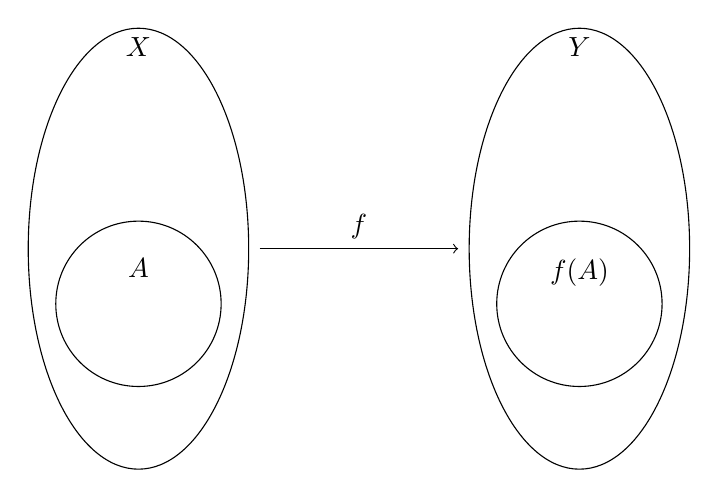
\begin{tikzpicture}[scale=0.7]
    \draw (-4.0,0.0) ellipse (2.0 and 4.0);
    \draw (-4.0,4.0) node[below]{$X$};
    \draw (-4.0,-1.0) circle (1.5);
    \draw (-4.0,0.0) node[below]{$A$};
    \draw (4.0,0.0) ellipse (2.0 and 4.0);
    \draw (4.0,4.0) node[below]{$Y$};
    \draw (4.0,-1.0) circle (1.5);
    \draw (4.0,0.0) node[below]{$f(A)$};
    \draw[->] (-1.8,0.0) -- (1.8,0.0);
    \draw (0.0,0.0) node[above]{$f$};
  \end{tikzpicture}
  \caption{Bild}
  \label{abb:abb:Bild}
\end{center}
\end{figure}

\begin{figure}[htbp]
\begin{center}
  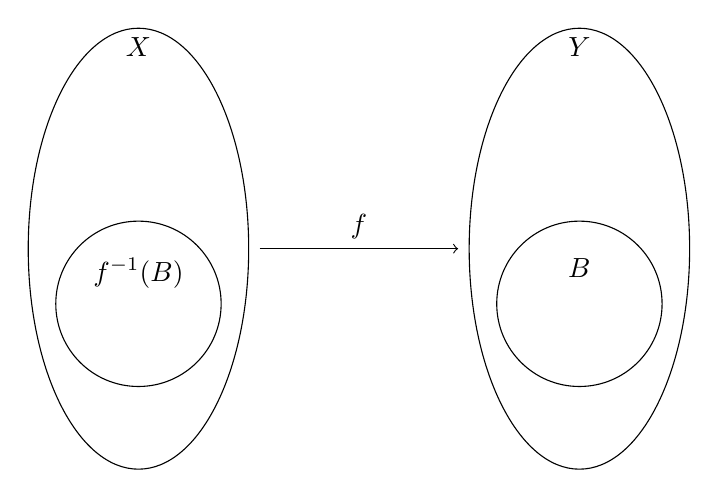
\begin{tikzpicture}[scale=0.7]
    \draw (-4.0,0.0) ellipse (2.0 and 4.0);
    \draw (-4.0,4.0) node[below]{$X$};
    \draw (-4.0,-1.0) circle (1.5);
    \draw (-4.0,0.0) node[below]{$f^{-1}(B)$};
    \draw (4.0,0.0) ellipse (2.0 and 4.0);
    \draw (4.0,4.0) node[below]{$Y$};
    \draw (4.0,-1.0) circle (1.5);
    \draw (4.0,0.0) node[below]{$B$};
    \draw[->] (-1.8,0.0) -- (1.8,0.0);
    \draw (0.0,0.0) node[above]{$f$};
  \end{tikzpicture}
  \caption{Urbild}
  \label{abb:abb:Urbild}
\end{center}
\end{figure}
\end{Unit} 

%% -----------------------------------------------------------------------------
\begin{Unit}[Bemerkung]
\label{bem:Abbildungen und Teilmengen}

Bei einer Abbildung $f: X \rightarrow Y$ und Teilmengen $A \subseteq X$ und 
$B \subseteq Y$ gilt für Bild und Urbild:

\begin{Bemerkung}
  Es sei $f: X \rightarrow Y$ eine Abbildung und $A \subseteq X$ und $B 
  \subseteq Y$, dann gelten \\
  (a) Die Menge $A \subseteq X$ ist eine Teilmenge der Urbildmenge vom Bild 
    von $A$:
    \begin{align}
      A \subseteq f^{-1}(f(A)) \ .
    \end{align}
  (b) Das Bild vom Urbild einer Menge $B \subseteq Y$ ist eine Teilmenge von 
    $B$:
    \begin{align}
      f(f^{-1}(B)) \subseteq B \ .
    \end{align}
\end{Bemerkung}

Beweis: \\
(a) Ist $a \in A$, dann ist $f(a) \in f(A)$ auf Grund der Definition von 
$f(A)$. Damit ist $a$ ein Element der Menge, deren Bilder in $f(A)$ sind. 
Diese Menge ist gemäß der Definition gleich dem Urbild von $f(A)$ 
($a \in \{x \in X \mid f(x) \in f(A)\} = f^{-1}(f(A))$). Damit ist 
$A \subseteq f^{-1}(f(A))$ gezeigt.

\begin{tabular}{l l l}
  & &  $a \in A$ \\
  & $\rightarrow$ &  $f(a) \in f(A)$\\
  & $\rightarrow$ & $a \in \{x \in X\ |\ f(x) \in f(A)\}$ = $f^{-1}(f(A))$ \\
  $\Rightarrow$ & & $A \subseteq f^{-1}(f(A))$\\
\end{tabular}

(b) Auf Grund der Definitionen gelten $f^{-1}(B) = \{x \in X \mid f(x) 
\in B\}$ und damit auch $f(f^{-1}(B)) = \{y \in Y \mid \exists a 
\in f^{-1}(B): f(a) = y\}$. Ist $b \in f(f^{-1}(B))$, dann existiert ein 
$a \in f^{-1}(B)$ mit $f(a) = b$. Da $a \in f^{-1}(b)$ ist, gilt somit 
$b = f(a) \in B$. Somit ist die Teilmengenbeziehung 
$f(f^{-1}(B)) \subseteq B$ gezeigt.

\begin{tabular}{l l l}
  & & $b \in f(f^{-1}(B))$ \\
  & $\rightarrow$ & $\exists a \in f^{-1}(B): f(a) = b$ \\
  & $\rightarrow$ & $b = f(a) \in B$ \\
  $\Rightarrow$ & & $f(f^{-1}(B)) \subseteq B$ \\
\end{tabular} 
\end{Unit}

%% -----------------------------------------------------------------------------
\begin{Unit}[Anmerkung] 
Die Umkehrungen gelten nicht, was an nachfolgenden Beispielen gesehen werden
kann, so dass dies (in der Regel) keine Mengengleichheiten sind! Später wird
gezeigt, unter welchen Bedingungen die Mengengleichheit doch gilt.
\end{Unit} 

%% -----------------------------------------------------------------------------
\begin{Unit}[Beispiel] 
  Gegeben sei die Abbildung $f: \RR \rightarrow \RR, x \mapsto f(x) = x^2$. 
  Dann gilt für $A = \{1\}$, $f(A) = \{1\}$ und $f^{-1}(f(A)) = \{1, -1\}$.
\end{Unit}

%% -----------------------------------------------------------------------------
\begin{Unit}[Beispiel] 
  Gegeben sei die Abbildung $f: \NN \rightarrow \NN, n \mapsto f(n) = 2n$. 
  Dann gilt für $B := \{1, 2\}$, $f^{-1}(B) = \{1\}$ und 
  $f(f^{-1}(B)) = \{2\}$
\end{Unit}

%% -----------------------------------------------------------------------------
\begin{Unit}[Bemerkung]
Für Verknüpfungen von Mengen und Abbildungen können Regeln angegeben werden.

\begin{Bemerkung}
Es seien $f: X \rightarrow Y$ eine Abbildung und $A, B \subseteq X$, dann gelten 
\\
(a) Das Bild des Durchschnitts ist Teilmenge des Durchschnitts der Bilder
  \begin{align}
    f(A \cap B) \subseteq f(A) \cap f(B) \ .
  \end{align}
(b) Das Bild der Vereinigung ist gleich dem Durchschnitt der Bilder.
  \begin{align}
    f(A \cup B) = f(A) \cup f(B) \ .
  \end{align}
\end{Bemerkung}

Beweis: Übung. Wieso gilt bei (a) nicht die Gleichheit?
\end{Unit}

%% -----------------------------------------------------------------------------
\begin{Unit}[Bemerkung]
Weiter gilt

\begin{Bemerkung}
  Es sei $f: X \rightarrow Y$ eine Abbildung, und $A, B \subseteq Y$, dann 
  gelten \\
  (a) Das Urbild des Durchschnitts ist gleich dem Durchschnitt der Urbilder:
    \begin{align}
      f^{-1} (A \cap B) = f^{-1} (A) \cap f^{-1} (B) \ .
    \end{align}
  (b) Das Urbild der Vereinigung ist gleich der Vereinigung der Urbilder:
    \begin{align}
      f^{-1} (A \cup B) = f^{-1} (A) \cup f^{-1} (B) \ .
    \end{align}
\end{Bemerkung}

Beweis: 

(a) Es sei $x \in f^{-1}(A \cap B)$, dann folgt daraus, dass $f(x) 
\in A \cap B$ ist. Somit ist $f(x) \in A$ und $f(x) \in B$. Somit gilt 
$x \in f^{-1}(A)$ und $x \in f^{-1}(B)$ und damit $x \in f^{-1}(A) 
\cap f^{-1}(B)$. Auch die Umkehrung gilt. Also gilt die gegenseitige
Teilmengenbeziehung und damit die Mengengleichheit. 

\begin{tabular}{l l}
  & $x \in f^{-1} (A \cap B)$ \\
  $\leftrightarrow$ & $f(x) \in A \cap B$ \\
  $\leftrightarrow$ & $f(x) \in A\land f(x) \in B$ \\
  $\leftrightarrow$ & $x \in f^{-1}(A) \land x \in f^{-1}(B)$ \\
  $\leftrightarrow$ & $x \in f^{-1}(A) \cap f^{-1}(B)$. 
\end{tabular} \qed

Beweis Teil( b) als Übung. 
\end{Unit}

%% -----------------------------------------------------------------------------
\begin{Unit}[Anmerkung Funktionen]
Funktionen sind eine andere Bezeichnung für Abbildungen. In der Algebra wird 
meist von Abbildungen gesprochen. Wenn die Mengen Zahlenmengen sind (in der 
Analysis beispielsweise reelle oder komplexe Zahlenmengen) wird meist von 
Funktionen gesprochen. 
\end{Unit} 
\Translation{Funktion}{function}

%%------------------------------------------------------------------------------
%% Abschnitt: Eigenschaften von Abbildungen
%%------------------------------------------------------------------------------
\section{Eigenschaften}
\label{sec:Abbildungen:Eigenschaften}

%% -----------------------------------------------------------------------------
\begin{Unit}[Definition injektiv, surjektiv und bijektiv]
Abbildung können bestimmte Eigenschaften haben.

\begin{Definition}
  Es sei $f: X \rightarrow Y$ eine Abbildung. Sie heißt \Begriff{injektiv} 
  oder \Begriff{eineindeutig}, wenn für zwei unterschiedliche Elemente 
  $x_1$ und $x_2$ von $X$ die Bilder $f(x_1)$ und $f(x_2)$ unterschiedlich 
  sind:
  \begin{align}
    \forall x_1, x_2 \in X: (f(x_1) = f(x_2)) \rightarrow ( x_1 = x_2 ) \\
    \forall x_1, x_2 \in X: ( x_1 \not= x_2 ) 
      \rightarrow (f(x_1) \not= f(x_2)) \ .
  \end{align}
  Sie heißt \Begriff{surjektiv}, falls es zu jedem Element $y \in Y$ ein 
  Element $x \in X$ gibt, mit $f(x) = y$:
  \begin{align}
    \forall (y \in Y): \exists (x \in X): f(x) = y \ .
  \end{align}
  Sie heißt \Begriff{bijektiv}, falls $f$ injektiv und surjektiv ist.
\end{Definition}
\Translation{injektiv}{injective}
\Translation{injektiv}{one-to-oneve}
\Translation{surjektiv}{surjective}
\Translation{surjektiv}{onto}
\Translation{bijektiv}{bijective}
\end{Unit} 

%% -----------------------------------------------------------------------------
\begin{Unit}[Bemerkung]
Ist die Abbildung injektiv, dann gibt es keine zwei Elemente in $X$, die auf 
das selbe Element in $Y$ abgebildet werden. Ist die Abbildung surjektiv, dann 
gibt es zu jedem Element von $Y$ mindestens ein Urbild in $X$. Damit gilt

\begin{Bemerkung}
  Es sei $f: X \rightarrow Y$ eine Abbildung. Es gelten
  \begin{align}
    f \text{ injektiv } :\Leftrightarrow\ \forall y \in Y: |f^{-1}(y)| 
      \leq 1 \\
    f \text{ surjektiv } :\Leftrightarrow\ \forall y \in Y: |f^{-1}(y)| 
      \geq 1\\
    f \text{ bijektiv } :\Leftrightarrow\ \forall y \in Y: |f^{-1}(y)| = 1
  \end{align}
\end{Bemerkung}

Bei einer surjektiven Abbildung $f: X \rightarrow Y$ gilt dann $f(X) = Y$.
\end{Unit}

%% -----------------------------------------------------------------------------
\begin{Unit}[Definition Umkehrabbildung]
Bei einer bijektiven Abbildung hat das Urbild jedes Elementes $y \in Y$ genau 
ein Element. Das bedeutet, dass jedem von $Y$ genau ein Element aus $X$ 
zugeordnet ist. Das ist die grundlegende Eigenschaft für eine Abbildung.

\begin{Definition}
  Es sei $f : X \rightarrow Y$ eine bijektive Abbildung, dann gibt es zu jedem 
  $y \in Y$ genau ein $x \in X$ mit $f(x) = y$ und es wird $f^{-1}(y) = x$
  geschrieben. 
  Die hierdurch definierte Abbildung $f^{-1}: Y \rightarrow X$ heißt 
  \Begriff{Umkehrabbildung} von $f$.
\end{Definition}
\Translation{Umkehrabbildung}{inverse map}
\end{Unit} 

%% -----------------------------------------------------------------------------
\begin{Unit}[Beispiel] 
  \begin{align}
    f: \NN \rightarrow \NN,\ n \mapsto f(n) = n + 1
  \end{align}
$f$ ist injektiv, jedoch nicht surjektiv.
\end{Unit}

%% -----------------------------------------------------------------------------
\begin{Unit}[Beispiel] 
  \begin{align}
    f: \NN \rightarrow \NN,\ n \mapsto f(n) = 2n
  \end{align}
$f$ ist injektiv, jedoch nicht surjektiv.
\end{Unit}

%% -----------------------------------------------------------------------------
\begin{Unit}[Beispiel] 
  \begin{align}
    f: \ZZ \rightarrow \ZZ,\ z \mapsto f(z) = z + 1
  \end{align}
  $f$ ist injektiv und surjektiv, also bijektiv.
\end{Unit}

%% -----------------------------------------------------------------------------
\begin{Unit}[Beispiel] 
\begin{align}
  f: \NN \rightarrow \ZZ, n \mapsto f(n) := 
  \begin{cases} 
    n/2      & \text{ falls }n{\ gerade } \\ 
    -(n-1)/2 & \text{ falls }n{\ ungerade } \ .
  \end{cases}
\end{align}
$f$ ist injektiv und surjektiv, also bijektiv.
\end{Unit}

%% -----------------------------------------------------------------------------
\begin{Unit}[Beispiel] 
\begin{align}
  f: \RR \rightarrow \RR,\ x \mapsto f(x) = x^2
\end{align}
Die Funktion $f$ ist nicht injektiv, da beispielsweise $f(1) = f(-1)$, jedoch 
$1 \not= -1$ gilt. Die Funktion $f$ ist auch nicht surjektiv, da $f(\RR) = 
\RR^+_0$. 
\end{Unit}

%% -----------------------------------------------------------------------------
\begin{Unit}[Beispiel] 
\begin{align}
  f: \RR^+_0 \rightarrow \RR^+_0, x \mapsto f(x) = \sqrt{x}
\end{align}
Die Funktion $f$ ist eine injektive und surjektive, also bijektive Abbildung.
\end{Unit}

%% -----------------------------------------------------------------------------
\begin{Unit}[Beispiel]  
  Es seien $M_i$ Mengen $(i = 1, 2, \ldots, n)$. Für jedes $i = 1,2,\ldots,n$ 
  sei die Abbildungen
  \begin{align}
    f_i : M_1 \times M_2 \times \cdots \times M_n \rightarrow M_i,\
      (x_1, x_2, \ldots, x_n) \mapsto x_i
  \end{align}
  definiert. Die Abbildungen $f_i$ sind surjektiv. Die Abbildung $f_i$ heißt 
  die $i$-te \Begriff{Projektion}.
\Translation{Projektion}{projection}
\end{Unit}

%% -----------------------------------------------------------------------------
\begin{Unit}[Beispiel]  
  Es seien $M$ eine Menge und $A$ eine Äquivalenzrelation. Durch 
  \begin{align}
    k: M \rightarrow M/A, x \mapsto [x]
  \end{align}
  wird eine Abbildung definiert. Sie ist surjektiv. Sie heißt 
  \Begriff{kanonische Abbildung}.
\Translation{kanonische Abbildung}{canonical mapping}
\end{Unit}

%% -----------------------------------------------------------------------------
\begin{Unit}[Beispiel]  
  Es sei $M$ eine Menge und $U \subseteq M$ eine Teilmenge von $M$. Durch
  \begin{align}
    \imath: U \rightarrow M, u \mapsto \imath(u) = u
  \end{align}
  wird eine Abbildung definiert. Die Abbildung ist injektiv. Sie heißt 
  \Begriff{Inklusionsabbildung} oder \Begriff{Einbettung} von $U$ in 
  $M$. Beispiele dafür sind die Einbettungen von $\NN$ in $\ZZ$, $\ZZ$ in $\QQ$ 
  und $\QQ$ in $\RR$.
\Translation{Inklusionsabbildung}{embedding}
\Translation{Einbettung}{embedding}
\end{Unit}

%% -----------------------------------------------------------------------------
\begin{Unit}[Definition konstante Abbildung] 
Eine einfache Abbildung ist eine konstante Abbildung.

\begin{Definition}[konstante Abbildung]
  Es sei $f: X \rightarrow Y$ eine Abbildung. Sie heißt \Begriff{konstant}
  oder \Begriff{konstante Abbildung}, falls alle Werte von $X$ auf das 
  selbe Element von $Y$ abgebildet werden.
  \begin{align}
    \forall x_1, x_2 \in X: f(x_1) = f(x_2)
  \end{align}
\end{Definition}
\Translation{konstante Abbildung}{constant mapping}
\end{Unit} 

%% -----------------------------------------------------------------------------
\begin{Unit}[Definition Einschränkung]
Eine Abbildung kann auf einen Teil des Definitionsbereiches eingeschränkt 
werden.
\begin{Definition}
  Eine Abbildung $g : U \rightarrow Y$ heißt \Begriff{Einschränkung} 
  von $f: X \rightarrow Y$, wenn $U$ eine Teilmenge von $X$ ist und für alle 
  Elemente $x$ aus $U$ $f(x) = g(x)$ gilt. 
  \begin{align}
    U \subseteq X \land \forall x \in U: f(x) = g(x) \ .
  \end{align}
  Es wird dann $g = f/U$ geschrieben.
\end{Definition}
\Translation{Einschränkung}{restriction}
\end{Unit} 

%% -----------------------------------------------------------------------------
\begin{Unit}[Definition Fortsetzung]
Ebenso wichtig ist es eine Abbildung über den gegebenen Definitionsbereich
fortzusetzen.
\begin{Definition}
  Eine Abbildung $g: O \rightarrow Y$ heißt \Begriff{Fortsetzung} von 
  $f: X \rightarrow Y$, wenn $O$ eine Obermenge von $X$ ist und $g/X = f$ 
  gilt.
  \begin{align}
    X \subseteq O \quad \land \quad g/X = f
  \end{align}
\end{Definition}
\Translation{Fortsetzung}{continuation}
\end{Unit} 

%% -----------------------------------------------------------------------------
\begin{Unit}[Beispiel] 
  Es sei die Abbildung $f : \RR \rightarrow \RR \backslash \{1\}, x \mapsto
  (x^2 -1 ) / (x - 1)$. Die Abbildung $g : \RR \rightarrow \RR, 
  x \mapsto x+1$ ist eine Fortsetzung von $f$.
\end{Unit}

%% -----------------------------------------------------------------------------
\begin{Unit}[Definition Identität]
Eine einfache Abbildung einer Menge in sich selber.
\begin{Definition}
  Es sei $f: X \rightarrow X$ eine Abbildung. Sie heißt \Begriff{Identität} 
  von $X$ $(id_X)$, falls jedes Element der Menge $X$ auf sich selbst 
  abgebildet wird:
  \begin{align}
    \forall x \in X: f(x) = x \ .
  \end{align}
\end{Definition}
\Translation{Identität}{identity mapping}
\end{Unit} 

%% -----------------------------------------------------------------------------
\begin{Unit}[Anmerkung] 
Eine Abbildung, deren Definitionsbereich $\NN$, die Menge der natürlichen 
Zahlen ist, heißt \Begriff{Folge}. Im allgemeinen wird eine Folge in der Form 
$(a_1, a_2, a_3, \ldots)$ oder $\{a_i\}_{i \in \NN}$ geschrieben.
\Translation{Folge}{sequence}
\end{Unit} 

%% -----------------------------------------------------------------------------
\begin{Unit}[Beispiel] 
  Es sei $f$ die Abbildung von $\NN$ nach $\ZZ$, die gegeben ist durch
  \begin{align}
    f:\NN \rightarrow \ZZ, z \mapsto z+1
  \end{align}
  Die Abbildung ist injektiv, aber nicht surjektiv. Der Definitionsbereich
  kann jedoch so angepasst werden, dass die Abbildung sowohl injektiv als
  auch surjektiv ist, also bijektiv. (Definitionsbereich $\ZZ$)
\end{Unit}

%% -----------------------------------------------------------------------------
\begin{Unit}[Beispiel] 
  Es sei die Abbildung
  \begin{align}
    f: \NN \rightarrow \ZZ, n \mapsto f(n) := 
    \begin{cases} 
      n/2      & \text{ falls }n{\ gerade } \\ 
      -(n-1)/2 & \text{ falls }n{\ ungerade } \ .
    \end{cases}
  \end{align}
  Die Abbildung $f$ ist bijektiv. Für den Nachweis müssen 
  Fallunterscheidungen durchgeführt werden.
\end{Unit}

%% -----------------------------------------------------------------------------
\begin{Unit}[Bemerkung]
In der Bemerkung \ref{bem:Abbildungen und Teilmengen} konnten nur die
Teilmengenbeziehungen $A \subseteq f^{-1}(f(A))$ und $f(f^{-1}(B))$ beweisen 
werden. Nun wird gezeigt, unter welchen Bedingungen sogar Mengengleichheit 
gilt.

\begin{Bemerkung} 
  Es sei $f: X \rightarrow Y$ eine Abbildung, $A \subseteq X$ und 
  $B \subseteq Y$ \\
  (a) Ist $f$ injektiv, dann gilt auch $f^{-1}(f(A)) \subseteq A$ und somit 
    $f^{-1}(f(A)) = A$. \\
  (b) Ist $f$ surjektiv, dann gilt auch $B \subseteq f(f^{-1}(B))$ und somit 
    $B = f(f^{-1}(B))$.
\end{Bemerkung}
Beweis: \\
(a) Es sei $a \in f^{-1}(f(A))$. Da $f^{-1}(f(A)) = \{ x \in X \mid f(x) \in 
  f(A)\}$ ist, gilt somit $f(a) \in f(A)$. Da $f(A) = \{ y \in Y \mid 
  \exists x \in A: f(x) = y\}$ ist, existiert ein $x \in A$ mit $f(x) 
  = f(a)$. Da $f$ injektiv ist, gilt $x = a$, also $a \in A$, da $x \in A$. 
  Somit ist $f^{-1}(f(A)) \subseteq A$. Zusammen mit Bemerkung 
  \ref{bem:Abbildungen und Teilmengen} ergibt sich die Mengengleichheit.

\begin{tabular}{l l l}
  &            & $a \in f^{-1}(f(A)) = \{x \in X \mid f(x) \in f(A)\}$ \\
  & $\rightarrow$ & $f(a) \in f(A) = \{y \in Y \mid \exists x \in A: f(x) 
    = y\}$ \\
  & $\rightarrow$ & $\exists x \in A: f(x) = f(a)$\\
  & $\rightarrow$ & $x = a$ (da f injektiv) \\
  & $\rightarrow$ & $a \in A$ \\
  $\Rightarrow$ & & $f^{-1}(f(A)) \subseteq A$
\end{tabular}

(b) Es sei $b \in B$, dann existiert ein $a \in X$ und $f(a) = b \in B$, 
da $f$ surjektiv ist. Damit ist $a \in f^{-1}(B)$ und somit $b = f(a) \in 
f(f^{-1}(B))$. Also gilt $B \subseteq f(f^{-1}(B))$. Zusammen mit Bemerkung 
\ref{bem:Abbildungen und Teilmengen} ergibt sich die Mengengleichheit.
  
\begin{tabular}{l l l}
  &               & $b \in B$ \\
  & $\rightarrow$ & $\exists a \in X: f(a) = b \in B$\\
  & $\rightarrow$ & $a \in f^{-1}(B)$\\
  & $\rightarrow$ & $b = f(a) \in f(f^{-1}(B))$ \\
  $\Rightarrow$ & & $B \subseteq f(f^{-1}(B))$
\end{tabular}
\end{Unit}

%% -----------------------------------------------------------------------------
\begin{Unit}[Definition Komposition von Abbildungen]
Zum Abschluss werden noch die Verknüpfungen von Abbildungen betrachtet.

\begin{Definition}
  Es seien $f : V \rightarrow W$ und $g : X \rightarrow Y$ Abbildungen mit $f(V) 
  \subseteq X$, so wird durch $(g \circ f)(v) := g(f(v))$ eine Abbildung $g 
  \circ f: V \rightarrow Y$ definiert. Diese Abbildung heißt 
  \Begriff{Komposition} von $f$ mit $g$.
\end{Definition}

Für die Umkehrabbildung der bijektiven Abbildung $f : X \rightarrow Y$ gilt 
$f^{-1} \circ f = id_X$ und $f \circ f^{-1} = id_Y$. Im Falle von $X = Y$ 
wird auch von der \Begriff{inversen Abbildung}\index{Abbildung gesprochen, 
inverse}.
\Translation{Komposition}{composition}
\Translation{inverse Abbildung}{inverse mapping}
\end{Unit} 

%% -----------------------------------------------------------------------------
\begin{Unit}[Beispiel] 
  Es seien
  \begin{align}
    f&: \RR \rightarrow \RR^+_0, x \mapsto f(x) = x^2 \\
    g&: \RR^+_0 \rightarrow \RR^+_0, x \mapsto g(x) = +\sqrt{x}
  \end{align}
  zwei Abbildungen. Die Abbildung $f$ ist surjektiv, aber nicht injektiv. Die 
  Abbildung $g$ ist bijektiv, mit der Umkehrabbildung
  \begin{align}
    g^{-1}:\RR^+_0 \rightarrow \RR^+_0, x \mapsto g(x) = x^2 \ .
  \end{align}
  Es gilt $f(\RR) = \RR^+_0$ und $g(\RR^+_0) = \RR^+_0$. Die Abbildung
  \begin{align}
    (g \circ f): \RR \rightarrow \RR^+_0, x \mapsto |x|
  \end{align}
  ist surjektiv, aber nicht injektiv. Die Abbildung
  \begin{align}
    (f \circ g):\RR^+_0 \rightarrow \RR^+_0, x \mapsto x
  \end{align}
  ist bijektiv, es gilt sogar, dass $f \circ g$ die Identität auf $\RR^+_0$ 
  ist.
\end{Unit}

%% -----------------------------------------------------------------------------
\begin{Unit}[Beispiel] 
  Es seien $f: \mg{R} \rightarrow \mg{R}, x \mapsto f(x) = x^2$ und 
  $g: \mg{R} \rightarrow \mg{R}, x \mapsto g(x) = x - 1$ zwei Abbildungen, 
  dann gelten
  \begin{align}
    (g \circ f)(x) = g(f(x)) = g(x^2) = x^2 - 1 \text{ und} \\
    (f \circ g)(x) = f(g(x)) = f(x-1) = (x-1)^2 = x^2 - 2x + 1 \ .
  \end{align}
\end{Unit}

%% -----------------------------------------------------------------------------
\begin{Unit}[Anmerkung] 
An diesem Beispiel ist zu sehen, dass in der Regel die Kompositionen 
$g \circ f$ und $f \circ g$ nicht identisch sind, die Komposition von 
Abbildungen also nicht kommutativ ist.

Die Komposition von Abbildungen ist assoziativ, das heißt, es gilt für 
Abbildungen $f : V \rightarrow W$, $g : W \rightarrow X$ und 
$h: X \rightarrow Y$:
\begin{align}
  h \circ (g \circ f) = (h \circ g) \circ f \ ,
\end{align}
da $(h \circ (g \circ f))(v) = h((g \circ f)(v)) = h(g(f(v))) = 
(h \circ g)(f(v)) = ((h \circ g) \circ f)(v)$ gilt.

Ist $f: X \rightarrow Y$ eine Abbildung, so gelten $id_Y \circ f = f$ und 
$f \circ id_X = f$.
\end{Unit} 

%% -----------------------------------------------------------------------------
\begin{Unit}[Beispiel] 
  Es seien $f$ und $g$ zwei Abbildungen:
  \begin{align}
    f:\RR^3 \rightarrow \RR^2: (x,y,z) \mapsto (x,y+z)\ \text{ und} \\
    g:\RR^2 \rightarrow \RR^2: (x,y) \mapsto (x+y,x-y) \ .
  \end{align}
  (a) Beweisen oder widerlegen Sie, dass die Abbildung $f$ injektiv und
    surjektiv ist. \\
  Wegen $f((0,0,1)) = (0,1) = f((0,1,0))$ ist nicht injektiv. \\
  Ist $(u,v) \in \RR^2$, so ist $f((u,v,0)) = (u,v)$ und somit ist die 
    Abbildung $f$ surjektiv.

  (b) Beweisen oder widerlegen Sie, dass die Abbildung $g$ injektiv und
    surjektiv ist. \\
  Aus $g((x_1,y_1)) = g((x_2,y_2))$ folgt $(x_1+y_1,x_1-y_1) = 
    (x_2+y_2,x_2-y_2)$ und somit $x_1 = x_2$ und $y_1 = y_2$. Also folgt 
    $(x_1,y_1) = (x_2,y_2)$, also ist $g$ injektiv.\\
  Ist $(u,v) \in \RR^2$, so ist $g(((u+v)/2,(u-v)/2)) = (u,v)$, also ist $g$
    surjektiv.

  (c) Bilden Sie die Abbildung $g \circ f$.\\
  Es gilt $(g \circ f)((x,y,z)) = g(f((x,y,z))) = g((x,y+z)) 
  = (x+y+z,x-y-z)$.

\end{Unit}

%%------------------------------------------------------------------------------
%% Abschnitt: Mengen von Abbildungen
%%------------------------------------------------------------------------------
\section{Mengen von Abbildungen}
\label{sec:Abbildungen:Mengen von Abbildungen}

%% -----------------------------------------------------------------------------
\begin{Unit}[Anmerkung] 
In den vorherigen Abschnitten wurden jeweils eine Abbildung und deren 
Eigenschaften betrachtet. Jetzt werden Mengen von Abbildungen betrachtet. 
Dazu jedoch zuerst ein kleines Beispiel.
\end{Unit} 

%% -----------------------------------------------------------------------------
\begin{Unit}[Beispiel] 
  Es seien $M = \{1,2\}$ und $N = \{1,2,3\}$ zwei Mengen mit zwei 
  beziehungsweise drei Elementen. Wie viele Abbildungen $f:M \rightarrow N$ 
  gibt es? Auf Grund der kleinen Anzahl von Elementen sind die Abbildungen 
  leicht zu bestimmen. Für jede Abbildung ist jeweils nur $f(1)$ und $f(2)$ 
  anzugeben, um die Abbildung zu bestimmen. Dies wird in der Tabelle 
  \ref{tbl:abb:Abbildungsvorschrift} aufgeführt. Es werden die verschiedenen 
  Abbildungen
  \begin{align}
    f_i : M \rightarrow N, x \mapsto f_i(x) \ .
  \end{align}
  angegeben.

  \begin{table}\begin{center}
    \begin{tabular} {c || c | c }
      i & $f_i(1)$ & $f_i(2)$ \\ \hline
      1 & 1 & 1 \\
      2 & 1 & 2 \\
      3 & 1 & 3 \\
      4 & 2 & 1 \\
      5 & 2 & 2 \\
      6 & 2 & 3 \\
      7 & 3 & 1 \\
      8 & 3 & 2 \\
      9 & 3 & 3 \\
    \end{tabular}
    \caption{Abbildungsvorschrift}
    \label{tbl:abb:Abbildungsvorschrift}
  \end{center} \end{table}

  Das bedeutet, dass es neun verschiedene Abbildungen von $M$ nach $N$ gibt.
\end{Unit}

%% -----------------------------------------------------------------------------
\begin{Unit}[Anmerkung] 
Dies ist nur ein kleines Beispiel, so dass es noch übersichtlich ist. Sind $M$ 
und $N$ endliche Mengen mit $m = |M|$ und $n = |N|$ Elementen, dann gibt es 
$n^m$ verschiedene Abbildungen.

Von den neun Abbildungen im obigen Beispiel ist keine Abbildung bijektiv. Dies 
scheitert bereits daran, dass $M$ und $N$ nicht gleich viele Elemente haben. 
Dies ist eine notwendige, jedoch keine hinreichende Bedingung. Wenn $M$ und 
$N$ zwei jeweils 3-elementige Mengen sind, dann gibt es insgesamt 27 
verschiedene Abbildungen. Von diesen Abbildungen sind jedoch nur sechs 
Abbildungen injektiv, surjektiv und damit bijektiv.
\end{Unit} 

%% -----------------------------------------------------------------------------
\begin{Unit}[Definition Menge von Abbildungen]
Jetzt wird eine Menge von Abbildungen definiert.

\begin{Definition}
  Es seien $M$ und $N$ zwei beliebige Mengen. Die Menge
  \begin{align}
    Abb(M,N) := \{f \mid f:M \rightarrow N\} 
  \end{align}
  heißt \Begriff{Menge der Abbildungen von $M$ nach $N$}. Ist $M = N$, so 
  wird kurz $Abb(M)$ statt $Abb(M,M)$ geschrieben und es heißt \Begriff
  {Menge der Abbildungen von M}.
  \begin{align}
    Bij(M) := \{f \in Abb(M) \mid f \text{ ist bijektiv } \} 
  \end{align}
  ist die \Begriff{Menge der bijektiven Abbildungen von M}.
\end{Definition} 
\end{Unit} 


\appendix
%\input{Grundbegriffe/app_A.tex}
\renewcommand{\mitAufgaben}{Nein}
\renewcommand{\mitLoesungen}{Ja}

\setcounter{section}{11}
%\section{Lösungen zu Kapitel \ref{cha:Gdl-K01-Sprache}}
\chapter{Lösungen zu den Aufgaben}
\section{Lösungen zu Kapitel \ref{cha:Gdl-K01-Sprache}}
%% =============================================================================
%% Mathematische Grundlagen - Grundbegriffe
%% Kapitel 01 - Sprache der Mathematik - Aufgaben und Lösungen
%% Autor: Andreas Zeh-Marschke
%% Datum: 2025-04-21
%% =============================================================================

%\ifthenelse{\equal{\mitAufgaben}{Ja}}{
%\section{Aufgaben}
%}{}
%\ifthenelse{\equal{\mitLoesungen}{Ja}}{
%\section{Lösungen zu Kapitel \ref{cha:Gdl-K01-Sprache}}
%}{}

%% -----------------------------------------------------------------------------
\ifthenelse{\equal{\mitAufgaben}{Ja}}{
\begin{Aufgabe}
Dies ist eine Aufgabe
\end{Aufgabe}
}{}

\ifthenelse{\equal{\mitLoesungen}{Ja}}{
\begin{Loesung}
Dies ist eine Lösung zu <unklar>
\end{Loesung}
}{}

%% -----------------------------------------------------------------------------
\ifthenelse{\equal{\mitAufgaben}{Ja}}{
\begin{Aufgabe}
Dies ist eine zweite Aufgabe
\end{Aufgabe}
}{}

\ifthenelse{\equal{\mitLoesungen}{Ja}}{
\begin{Loesung}
Dies ist eine zweite Lösung
\end{Loesung}
}{}



% - - - - - - - - - - - - - - - - - - - - - - - - - - - - - - - - - - - - - - -
\printbibliography  %% --- Literaturverzeichnis ---
\PRINTINDEXES

\end{document}
